\chapter{Top Asymmetry Measurements}
\label{chap:afb}

This chapter will describe the measurements of several asymmetries in
events where a top-antitop ($\ttbar$) pair decays to a two-lepton
final state ($2\ell$). This work was performed using the CMS
experiment during Run I of the LHC, at both 7 TeV and 8 TeV
center-of-mass energies;
I will focus on the 8 TeV results, and in particular, my work on the
unfolding technique. The 8 TeV analysis led to two publications, which
are References \cite{chargeasym} and \cite{spincorrpol}.

% Make sure to do a final check for past vs. present tense

\section{Motivation}
\label{sec:afb:motivation}

As mentioned in Section \ref{ssec:SM:description}, the top quark is the
heaviest known elementary particle, with a mass of $\sim 173$ GeV
\cite{pdg}. This large mass gives the top quark a number of properties
that make it uniquely interesting to study.

In general, a particle's lifetime -- how long it tends to last before
decaying -- is inversely related to its mass \cite{griffiths}.
The top quark being so heavy, it has an extremely short lifetime
of $\mathcal{O} (10^{-25})$ seconds. This is shorter than the timescales on
which hadronization ($10^{-24}$s) and spin decorrelation ($10^{-21}$s)
normally occur \cite{pdg,spindecorrelation}, processes that normally
wipe out some information about a quark. Since the top quark decays
before they can happen, it passes on information about its spin
correlation and polarization to its decay products. So studying the decay
products of the top quark is one of the only ways we have to measure
these properties from a bare, unbound quark.

Additionally, the top quark's large mass places it on the edge of
unexplored territory. Because the likelihood of a particular decay is
proportional to the mass difference between the particles involved,
many of the heavy new particles predicted by BSM theories would have strong
couplings to the top quark.
These couplings would naturally cause some of the top quark's
properties to deviate from the value predicted by the SM. Thus, it is
important to make precise measurements of properties such as charge
asymmetry to tease out any links to possible new physics.

There are a few different final states that can result from the decay
of $\ttbar$ pairs. The top decays to a W boson and a $b$ quark, and
the W boson can decay to quarks or to a lepton and a neutrino. The
hadronic W decay has a higher cross-section than the leptonic decay \cite{pdg},
meaning that the more hadrons in the final state, the more data we
would have to work with. Nevertheless, the CMS detector was designed
with high-precision lepton reconstruction in mind, and precision is
important to these asymmetry measurements. So we chose to study the two-lepton
final state, valuing the precision of the lepton reconstruction over
higher statistics. The production of a top-antitop pair and its decay
to a dilepton final state is depicted in Figure
\ref{fig:afb:feynmandiagram}.

% Feynman diagram, made by yours truly
\begin{figure}
\centering
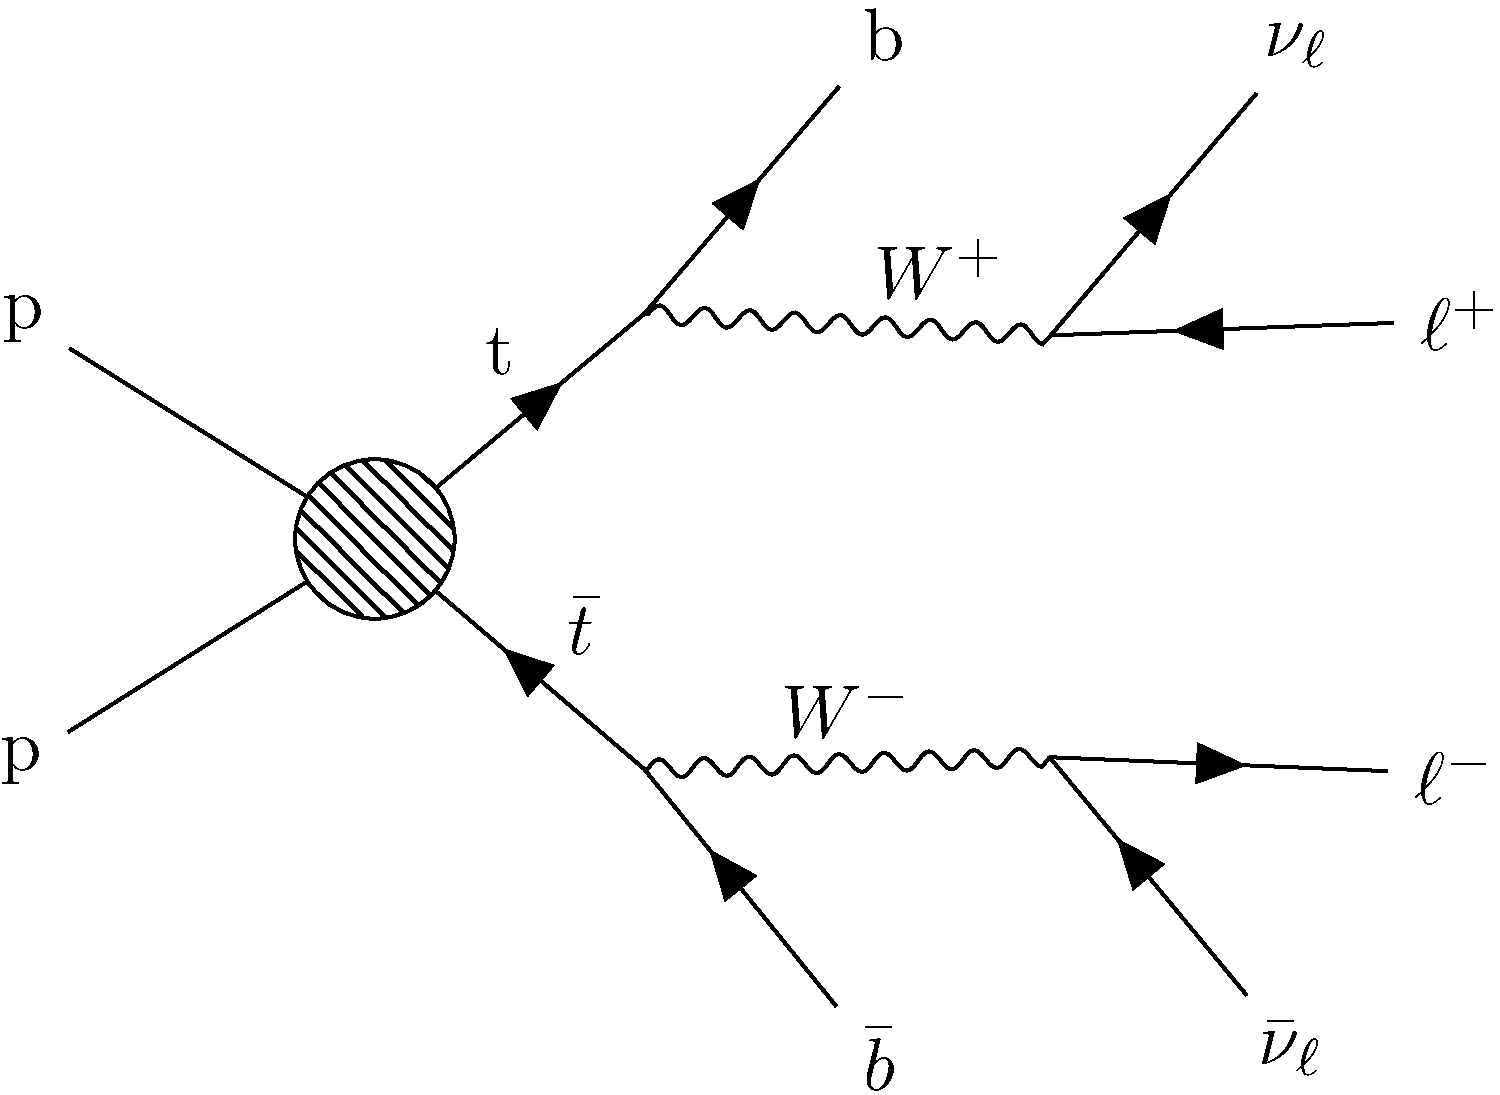
\includegraphics[width=0.6\textwidth]{figures/feynmandiagram_afb.pdf}
\caption[Feynman diagram showing a proton-proton collision that
  produces a $\ttbar$ pair, which subsequently decays
  dileptonically. The two leptons ($\ell$) are not necessarily the
  same flavor.]
  {Feynman diagram showing a proton-proton collision that produces
  a $\ttbar$ pair, which subsequently decays dileptonically. The two
  leptons ($\ell$) are not necessarily the same flavor. This
  diagram was made using the Tikz-Feynman package \cite{tikzfeynman}.}
\label{fig:afb:feynmandiagram}
\end{figure}

\section{Previous Measurements}
\label{sec:afb:tevatron}

The CDF and D0 experiments on the Tevatron collider at Fermilab made
several previous measurements of top charge asymmetry
\cite{cdfchargeasym1,d0chargeasym1, cdfchargeasym2,d0chargeasym2}, and
CDF, D0, and ATLAS made prior measurements of top spin correlation and
polarization
\cite{cdfspincorr,d0spincorr1,d0spincorr2,d0pol,atlaspol,atlasspincorr}. The
early charge asymmetry measurements
\cite{cdfchargeasym1,d0chargeasym1} were particularly interesting,
because they revealed a $2\sigma$ deviation from the SM expectation,
though later results \cite{cdfchargeasym2,d0chargeasym2} showed a
reduced discrepancy. During Run I of the LHC, it was natural to want to
confirm and extend the Tevatron measurements, and to cross-check the
ATLAS measurements.

The Tevatron collided beams of protons against beams of
antiprotons. When such $p\bar{p}$ collisions produce
$\ttbar$ pairs, we expect the top will tend to travel more along the direction
of the proton beam, and the antitop will tend to travel
more along the direction of the antiproton beam, so that the
difference in their rapidities tends to be positive ($y_t - y_{\bar{t}} > 0$).
This case was called ``forward'', and the reverse was called
``backward''. Thus, given a number of $\ttbar$
events from the Tevatron, we can define a forward-backward
asymmetry by subtracting the number of backward events from the number
of forward ones:

\begin{equation}
A_{FB} = \asymmetry{\Delta y}{0}
\end{equation}

However, the LHC is a proton-proton collider, and as such, there is no
naturally favored direction for the top or antitop to travel. As the
next section will explain, we must define ``forward'' and ``backward''
events somewhat differently.

\section{Asymmetry Variables}
\label{sec:afb:variables}

In this analysis, we evaluated six different asymmetries in $\ttdilep$
events, including two charge asymmetries, one polarization variable,
and three measures of spin correlation. If any of these
variables deviate from their expected SM values, it could potentially
be a sign of new physics.

\subsection{Definitions}
\label{ssec:afb:variables}

% Top charge asymmetry %%%%%%%%%%%
As at the Tevatron, the top charge asymmetry was measured at CMS using
the rapidity of the top quarks. However, absent a natural direction
for the top and antitop to travel, we categorized events as
``forward'' and ``backward'' based on which quark had a higher
absolute value of rapidity. Thus we define our \textbf{top charge
asymmetry} as:
\begin{equation}
A_C = \asymmetry{|y_t|}{|y_{\bar{t}}|}
\label{eq:afb:topchargeasym}
\end{equation}

% Leptonic charge asymmetry %%%%%%%%
In addition to the top charge asymmetry, we define a similar
\textbf{leptonic charge asymmetry} to be:
\begin{equation}
A_C^{lep} = \asymmetry{|\eta_{\ell^+}|}{|\eta_{\ell^-}|}
\end{equation}
Though similar to the top charge asymmetry, this variable
is based purely on the pseudorapidity of the leptons produced in the
decay. We may use the leptons as a proxy for the tops because we
expect their direction to be correlated with the directions of their
parent tops. One advantage of using only the leptons is that it obviates the
need to reconstruct the $\ttbar$ system, as described in Sec.
\ref{sec:afb:selections}, thereby allowing us to include more events in
our calculation of this variable. However, this variable also has some
dependence on the polarization, so it is not fully correlated with $A_C$.

% INTERLUDE: Helicity angle %%%%%%%%%%%
Before proceding further, we must define the \emph{helicity angle}, which
will be used in the next two asymmetry variables.
The helicity angle $\theta^*_{\ell}$ is defined as the angle
a charged lepton makes in the rest frame of its parent top,
relative to the parent top's direction in the $\ttbar$ center-of-mass
(CM) reference frame. This angle may be defined separately for the
positive and negative charged lepton in an event.

% Top polarization %%%%%%%%%%%%%%
The \textbf{top polarization} is an asymmetry based on the helicity
angles of the charged leptons, and is given by:
\begin{equation}
A_{P} = \asymmetry{\cos(\theta^*_{\ell})}{0}
\end{equation}
We use both the positively and negatively charged leptons in this
asymmetry measurement. A different, commonly used
polarization variable, $P$, can be calculated as $P = 2 A_P = 2(
A_{P+} + A_{P-})$, if we assume CP-invariance.

% Top spin correlation %%%%%%%%%
Our \textbf{top spin correlation} asymmetry, which also depends on the
lepton helicity angles, is defined as:
\begin{equation}
A_{c1c2} = \asymmetry{\cos(\theta^*_{\ell^+}) \times \cos(\theta^*_{\ell^-})}{0}
\end{equation}
From this variable, we may also obtain the $C$ spin correlation
coefficient, which is given by $C = -4 \times A_{c1c2}$ \cite{spincorrpolcoeff}.

% Lepton azimuthal asymmetry %%%%%
We also obtain an indirect measurement of the spin correlation using
the \textbf{lepton azimuthal asymmetry}. This variable depends on the
azimuthal angle between the two leptons, and is defined as:
\begin{equation}
A_{\Delta\phi} = \asymmetry{\Delta\phi_{\ell^+\ell^-}}{\pi/2}
\end{equation}
As with the leptonic charge asymmetry, this variable also relies
solely on the charged leptons, and does not require reconstruction of
the $\ttbar$ system, permitting us to use more events than are
available for the top spin correlation.

% Lepton opening angle %%%%%%%%%
Finally, we define our \textbf{lepton opening angle} asymmetry as:
\begin{equation}
A_{\cos\phi} = \asymmetry{\cos(\phi_{\ell\ell})}{0}
\end{equation}
This variable is based on the opening angle between the two leptons in
their respective parent top reference frames. From this measured
asymmetry, we can calculate the $D$ spin correlation coefficient to be
$D = -2 \times A_{\cos\phi}$ \cite{spincorrpolcoeff}.

\subsection{Differential Measurements}
\label{ssec:afb:varsdifferential}

In addition to measuring the above six asymmetries in one dimension
(\emph{inclusively}), we also measure them in two dimensions
(\emph{differentially}), against other physical variables.
We chose to make differential measurements because the CDF charge asymmetry
discrepancy was more pronounced at $\ttbar$ invariant masses above 450
GeV than below 450 GeV \cite{cdfchargeasym1}. If similar behavior
occurs at CMS, in any variable, we would like to observe it. We
measured all six of our asymmetry variables differentially with
respect to the $\ttbar$ invariant mass ($m_{\ttbar}$), absolute
rapidity ($|y_{\ttbar}|$), and transverse momentum ($p_T^{\ttbar}$).

\section{Datasets and Triggers}
\label{sec:afb:datatrig}

For this analysis, we used 19.5 fb\textsuperscript{-1} of data from
the 8 TeV portion of CMS Run I, encompassing the 2012A through 2012D
eras. Because the analysis focused on a process that produced two
leptons in the final state, we used the dilepton datasets from that
period. A complete list is given in Table \ref{tab:afb:datasamples}.

%% Table of data samples. Taken from AN-14-246. Believed unpublished so far %%%%%%%
\begin{table}[!ht]
\begin{center}
\caption{List of CMS datasets used.}
\label{tab:afb:datasamples}
{\footnotesize
\begin{tabular}{l|r}
\hline
Dataset Name & run range \\
\hline\hline
Dilepton Samples \\
\hline

  /DoubleMu/Run2012A-13Jul2012-v1/AOD &  190456-193621 \\
  /DoubleElectron/Run2012A-13Jul2012-v1/AOD & 190456-193621  \\
  /MuEG/Run2012A-13Jul2012-v1/AOD & 190456-193621 \\

  /DoubleMu/Run2012A-recover-06Aug2012-v1/AOD & 190949 190945 190906 190895 190782 \\
  /DoubleElectron/Run2012A-recover-06Aug2012-v1/AOD & 190949 190945 190906 190895 190782 \\
  /MuEG/Run2012A-recover-06Aug2012-v1/AOD & 190949 190945 190906 190895 190782\\

  /DoubleElectron/Run2012B-13Jul2012-v1/AOD  & 193834-196531 \\
  /DoubleMu/Run2012B-13Jul2012-v1/AOD  & 193834-196531  \\
  /MuEG/Run2012B-13Jul2012-v1/AOD  & 193834-196531  \\

  /DoubleElectron/Run2012C-24Aug2012-v1/AOD &  197770- 198913 \\
  /DoubleMu/Run2012C-24Aug2012-v1/AOD &  197770- 198913 \\
  /MuEG/Run2012C-24Aug2012-v1/AOD &  197770- 198913 \\

  /DoubleElectron/Run2012C-PromptReco-v2/AOD & 198934 - 203755  \\
  /DoubleMu/Run2012C-PromptReco-v2/AOD &  198934 - 203755 \\
  /MuEG/Run2012C-PromptReco-v2/AOD &  198934 - 203755 \\

  /DoubleElectron/Run2012D-PromptReco-v1/AOD & 203768 - 208686 \\
  /DoubleMu/Run2012D-PromptReco-v1/AOD & 203768 - 208686 \\
  /MuEG/Run2012D-PromptReco-v1/AOD & 203768 - 208686 \\

\hline
\end{tabular}
}
\end{center}
\end{table}

We used several Monte Carlo datasets to model both the $\ttdilep$
process and any potential background processes. A list of all Monte
Carlo datasets used is given in Table \ref{tab:afb:mcsamples}.

%% Table of MC samples. Adapted from AN-14-246. Believed unpublished so far %%%%%%%
\begin{table}[pht]
\begin{center}
\caption{List of CMS Monte Carlo samples used.}
\label{tab:afb:mcsamples}
{\footnotesize
\begin{tabular}{l|l|c}
\hline
\multicolumn{3}{c}{With Pileup: Processed dataset name is} \\
\multicolumn{3}{c}{(53) Summer12\_DR53X-PU\_S10\_START53\_V7A-v*/AODSIM} \\
\hline
 Description                     &   Primary Dataset Name   & cross-section [pb]\\
\hline
$\ttbar$                                                     &   /TT\_TuneZ2Star\_8TeV-mcatnlo (S3)                            & 234 \\
$\ttbar$ (alternative)                                           &   /TT\_CT10\_TuneZ2Star\_8TeV-powheg-tauola (53)           & 234 \\
W $\rightarrow$ $\ell\nu$+ jets                &   /WJetsToLNu\_TuneZ2Star\_8TeV-madgraph-tarball                             & 37509\\
W $\rightarrow$ $\ell\nu$+1 jets               &   /W1JetsToLNu\_TuneZ2Star\_8TeV-madgraph-tauola (53)                        &  6663  \\
W $\rightarrow$ $\ell\nu$+2 jets               &   /W2JetsToLNu\_TuneZ2Star\_8TeV-madgraph-tauola (53)                        &  2159 \\
W $\rightarrow$ $\ell\nu$+3 jets               &   /W3JetsToLNu\_TuneZ2Star\_8TeV-madgraph-tauola (53)                        &   640 \\
W $\rightarrow$ $\ell\nu$+$\geq 4$ jets        &   /W4JetsToLNu\_TuneZ2Star\_8TeV-madgraph-tauola (53)                        &   264 \\
WW      & /WWJetsTo2L2Nu\_TuneZ2star\_8TeV-madgraph-tauola (53) &   5.8123\\
WZ      & /WZJetsTo3LNu\_TuneZ2\_8TeV-madgraph-tauola (53)              &   1.0575\\
        & /WZJetsTo2L2Q\_TuneZ2star\_8TeV-madgraph-tauola (53)          &   2.206\\
ZZ      & /ZZJetsTo2L2Nu\_TuneZ2star\_8TeV-madgraph-tauola (53)         &   0.365\\
        & /ZZJetsTo4L\_TuneZ2star\_8TeV-madgraph-tauola (53)            &   0.176908\\
        & /ZZJetsTo2L2Q\_TuneZ2star\_8TeV-madgraph-tauola (53)          &   2.4487\\
$WG^{*}$  & /WGstarToLNu2E\_TuneZ2star\_8TeV-madgraph-tauola (53)          &  \\
        & /WGstarToLNu2Mu\_TuneZ2star\_8TeV-madgraph-tauola (53)          &  \\
        & /WGstarToLNu2Tau\_TuneZ2star\_8TeV-madgraph-tauola (53)          &  \\
$t$ ($s$-chan)                           &   /T\_TuneZ2Star\_s-channel\_8TeV-powheg-tauola (53)                        &  3.9 \\
$\bar{t}$ ($s$-chan)                     &   /Tbar\_TuneZ2Star\_s-channel\_8TeV-powheg-tauola (53)                      &  1.8 \\
$t$ ($t$-chan)                           &   /T\_TuneZ2Star\_t-channel\_8TeV-powheg-tauola (53)                         &  55.5 \\
$\bar{t}$ ($t$-chan)                     &   /Tbar\_TuneZ2Star\_t-channel\_8TeV-powheg-tauola (53)                      &  30.0 \\
$tW$                                     &   /T\_TuneZ2Star\_tW-channel-DR\_8TeV-powheg-tauola (53)                     &  11.2 \\
$\bar{t} W$                               &   /Tbar\_TuneZ2Star\_tW-channel-DR\_8TeV-powheg-tauola (53)                  &  11.2 \\
Z/$\gamma^* \rightarrow \ell \ell$      & /DYJetsToLL\_TuneZ2Star\_M-10To50filter\_8TeV-madgraph (53)                   &  860.5 \\
Z/$\gamma^* \rightarrow \ell \ell$      & /DYJetsToLL\_TuneZ2Star\_M-50\_8TeV-madgraph-tarball (53)                   &  3532.8 \\
Z/$\gamma^* \rightarrow \ell \ell$+$\geq 1$ jets       & /DY1JetsToLL\_M-50\_TuneZ2Star\_8TeV-madgraph (53)                   &  671.83 \\
Z/$\gamma^* \rightarrow \ell \ell$+$\geq 2$ jets       & /DY2JetsToLL\_M-50\_TuneZ2Star\_8TeV-madgraph (53)                   &  216.76 \\
Z/$\gamma^* \rightarrow \ell \ell$+$\geq 3$ jets       & /DY3JetsToLL\_M-50\_TuneZ2Star\_8TeV-madgraph (53)                   &  61.2 \\
Z/$\gamma^* \rightarrow \ell \ell$+$\geq 4$ jets       & /DY4JetsToLL\_M-50\_TuneZ2Star\_8TeV-madgraph (53)                   &  27.6 \\
$\ttbar W$                                       &   /TTW\_TuneZ2Star\_8TeV-madgraph (53)                   &  0.23 \\
$\ttbar Z$                                       &   /TTZ\_TuneZ2Star\_8TeV-madgraph (53)                   &  0.21 \\
$\ttbar \gamma$                      &   /TTGJets\_TuneZ2Star\_8TeV-madgraph (53)            &  2.166 \\
$\ttbar W W$                                     &   /TTWW\_TuneZ2Star\_8TeV-madgraph (53)        &  0.002037  \\
WWW     & /WWW\_TuneZ2Star\_8TeV-madgraph (53)                  & 0.08058 \\
WWZ     & /WWZNoGstar\_TuneZ2Star\_8TeV-madgraph (53)           & 0.05798 \\
WZZ     & /WZZNoGstar\_TuneZ2Star\_8TeV-madgraph (53)           & 0.01698 \\
ZZZ     & /ZZZNoGstar\_TuneZ2Star\_8TeV-madgraph (53)           & 0.0055269 \\
WWG     & / WWGJets\_TuneZ2Star\_8TeV-madgraph (53)             & 0.528 \\
\hline\hline
\end{tabular}
}
\end{center}
\end{table}

To select events from the datasets listed in
\ref{tab:afb:datasamples}, we used a set of dilepton triggers that
would capture the four possible dilepton flavors. These triggers are
listed in table \ref{tab:afb:triggers}.

%% Table of triggers used. Taken from AN-14-246. Believed unpublished so far %%%%%%%
\begin{table}[!ht]
\begin{center}
\caption{List of triggers used.}
\label{tab:afb:triggers}
\begin{tabular}{l}
\hline\hline
Triggers   \\
\hline\hline
Dilepton Sample \\
\hline
\footnotesize{\verb=HLT_Mu17_Mu8_v*=}\\
\footnotesize{\verb=HLT_Mu17_Ele8_CaloIdT_CaloIsoVL_TrkIdVL_TrkIsoVL_v*=}\\
\footnotesize{\verb=HLT_Mu8_Ele17_CaloIdT_CaloIsoVL_TrkIdVL_TrkIsoVL*=}\\
\footnotesize{\verb=HLT_Ele17_CaloIdT_CaloIsoVL_TrkIdVL_TrkIsoVL_Ele8_CaloIdT_CaloIsoVL_TrkIdVL_TrkIsoVL_v*=}\\
\hline
\end{tabular}
\end{center}
\end{table}

\section{Object and Event Selection}
\label{sec:afb:selections}

We employed a set of physics object and event selections designed to
accept as many $\ttdilep$ events as possible while minimizing the
number of background events selected.

\subsection{Object Definitions}
\label{ssec:afb:objdefs}

For the purpose of our analysis, we consider a lepton to mean an
electron or muon. Taus are excluded because of the difficulties in
correctly reconstructing and identifying them. We define our leptons
using the following criteria:

\begin{itemize}
\item Electrons and muons are defined using the recommended
  2012 identification criteria provided by their respective Physics Object
  Groups (POGs) within CMS. Specifically, electrons use the
  recommended medium working point (WP), and muons use the recommended
  tight WP.
\item We require the leptons to have $p_T > 20$ GeV and $|\eta| < 2.4$.
\item We use particle flow-based isolation within a cone of $\Delta R
  < 0.3$, where absolute isolation must be $< 5$ GeV, and relative
  isolation (isolation / $p_T$) must be $< 0.15$. % AN talks about PU corrections too
\item The PF lepton and the reconstructed lepton must have $p_T$ that
  differ by $< 10$ GeV.
\item For electrons, we require $E / p_{in} < 4$. % E_calo / p_inner tracker < 4
\end{itemize}

Jets are defined using particle flow. They must have $p_T > 30$ GeV
and $|\eta| < 2.4$. They must pass the tight Multi-Variate Analysis
(MVA) pileup ID, and they must be separated from leptons by $\Delta R
> 0.4$. B-tagging of jets is done using the Combined Secondary Vertex
(CSV) medium working point. MET is computed by summing up the vector
momenta of all PF particles, and multiplying by $-1$.

\subsection{Event Selections}
\label{ssec:afb:eventsel}

Using the above object definitions, we select events with exactly
two leptons of opposite-sign charge, and at least two jets, including at
least one b-tagged jet. Some additional requirements on these objects
include:

\begin{itemize}
\item To suppress events with low-mass resonances, we require the
  dilepton invariant mass $M_{\ell\ell} > 20$ GeV.
\item For events where the leptons have the same flavor, we require
  $|M_{\ell\ell} - M_Z| > 15$ GeV to exclude dileptons produced by the
  Drell-Yan (DY) process.
\item We also require MET $> 40$ GeV in same-flavor events, which
  further helps to reduce the DY background.
\end{itemize}

Additionally, we clean our data events using a number of standard
event filters. These filters are:

\begin{itemize}
\item At least one primary vertex
\item Beam scraping events
\item Tracking failure
\item HBHE noise filter
\item EE noise filter
\item ECAL/HCAL laser events
\item CSCHaloFilter
\item Anomalous $\rho$
\end{itemize}

\subsection{Corrections}
\label{ssec:afb:evtweights}

We make several corrections to our data to remove spurious effects,
and to our Monte Carlo simulations to more accurately reflect the
properties of the data. In particular:

\begin{itemize}
\item We measure the efficiencies of our chosen triggers
  vs. $p_T$ and $\eta$, and reweight
  MC events to reflect these efficiencies. The measurement technique
  is described below.
\item We use lepton identification and isolation efficiencies measured
  in a previous but related analysis \cite{run1stop1l}. As these values agree well with
  the efficiencies of our MC, we apply no correction, but we do assign
  a systematic uncertainty, as described in Section
  \ref{sec:afb:systematics}.
\item We correct the MC for the efficiency of b-tagging using the CSV
  discriminator reshaping method.
\item We apply the standard Jet Energy Corrections (JECs).
\item JECs are propagated to the MET calculation for jets with $p_T >
  10$ GeV, and the MET is also corrected to remove modulation in $\phi$.
\end{itemize}

\subsubsection*{Trigger efficiency measurements} % Should this section be moved to under "datasets and triggers"?
We measure the efficiencies of the dilepton triggers listed in Table
\ref{tab:afb:triggers} using a method called \emph{tag-and-probe}. The
essence of this method is that the process $Z \rightarrow \ell\ell$
is very clean to reconstruct and has a much higher cross section than its
backgrounds. We begin by selecting pairs of leptons that are consistent with
a Z boson origin. We require that one of the leptons pass some very tight
selection (we call this lepton a tag). The other lepton must pass some
looser selection (we call it a probe). The efficiency of a lepton
trigger is thus given by the fraction of tag-probe pairs where the
probe passes the trigger.

For this analysis, tags must pass our full analysis selections, must
have $p_T > 30$ GeV and $|\eta| < 2.1$, and must be matched to the
dilepton trigger. Probes need only pass our analysis
selections. A tag-probe pair must have opposite charge, and must have an invariant mass within 15
GeV of the Z boson mass. We evaluate the efficiencies of the leading
and trailing legs of the dilepton triggers separately. The muon trigger
efficiencies are given in Tables \ref{tab:afb:trigeff:mu8} and
\ref{tab:afb:trigeff:mu17}, and the electron trigger efficiencies are
given in Tables \ref{tab:afb:trigeff:ele8} and \ref{tab:afb:trigeff:ele17}.

% Mu8 leg trigger efficiency
\begin{table}[htbp]
\begin{center}
\footnotesize
\caption{Measured efficiency of the Mu8 leg of the
HLT\_Mu17\_Mu8\_v* trigger. Uncertainties are statistical only.}
\label{tab:afb:trigeff:mu8}
\begin{tabular}{c|c|c|c|c}
\hline
\hline
  $p_T$ range [GeV] & $|\eta|<0.8$ & $0.8<|\eta|<1.2$ & $1.2<|\eta|<2.1$  & $2.1<|\eta|<2.5$\\
\hline
  20 -  30  & 0.979 $\pm$ 0.001 & 0.948 $\pm$ 0.002 & 0.945 $\pm$ 0.002 & 0.925 $\pm$ 0.003\\
  30 -  40  & 0.978 $\pm$ 0.001 & 0.949 $\pm$ 0.001 & 0.939 $\pm$ 0.001 & 0.931 $\pm$ 0.002\\
  40 -  60  & 0.978 $\pm$ 0.001 & 0.948 $\pm$ 0.001 & 0.935 $\pm$ 0.001 & 0.934 $\pm$ 0.002\\
  $>$60     & 0.979 $\pm$ 0.002 & 0.949 $\pm$ 0.004 & 0.930 $\pm$ 0.004 & 0.932 $\pm$ 0.007\\
\hline
\hline
\end{tabular}
\end{center}
\end{table}

% Mu17 leg trigger efficiency
\begin{table}[htbp]
\begin{center}
\footnotesize
\caption{Measured efficiency of the Mu17 leg of the
HLT\_Mu17\_Mu8\_v* trigger. Uncertainties are statistical only.}
\label{tab:afb:trigeff:mu17}
\begin{tabular}{c|c|c|c|c}
\hline
\hline
  $p_T$ range [GeV] & $|\eta|<0.8$ & $0.8<|\eta|<1.2$ & $1.2<|\eta|<2.1$  & $2.1<|\eta|<2.5$\\
\hline
  20 -  30  & 0.977 $\pm$ 0.001 & 0.937 $\pm$ 0.003 & 0.931 $\pm$ 0.002 & 0.863 $\pm$ 0.004\\
  30 -  40  & 0.976 $\pm$ 0.001 & 0.939 $\pm$ 0.001 & 0.928 $\pm$ 0.001 & 0.890 $\pm$ 0.002\\
  40 -  60  & 0.977 $\pm$ 0.001 & 0.939 $\pm$ 0.001 & 0.926 $\pm$ 0.001 & 0.899 $\pm$ 0.002\\
  $>$60     & 0.978 $\pm$ 0.002 & 0.941 $\pm$ 0.004 & 0.922 $\pm$ 0.004 & 0.904 $\pm$ 0.008\\
\hline
\hline
\end{tabular}
\end{center}
\end{table}

% Ele8 leg trigger efficiency
\begin{table}[htbp]
\begin{center}
\footnotesize
\caption{Measured efficiency of the Ele8 leg of the
HLT\_Ele17\_CaloIdT\_CaloIsoVL\_TrkIdVL\_TrkIsoVL\_Ele8\_CaloIdT\_CaloIsoVL\_TrkIdVL\_TrkIsoVL\_v*
trigger. Uncertainties are statistical only.}
\label{tab:afb:trigeff:ele8}
\begin{tabular}{c|c|c}
\hline
\hline
  $p_T$ range [GeV] & $|\eta|<1.5$ & $1.5<|\eta|<2.5$\\
\hline
  20 -  30  & 0.964 $\pm$ 0.001 & 0.979 $\pm$ 0.001\\
  30 -  40  & 0.978 $\pm$ 0.001 & 0.986 $\pm$ 0.001\\
  40 -  60  & 0.982 $\pm$ 0.001 & 0.989 $\pm$ 0.001\\
  $>$60     & 0.985 $\pm$ 0.001 & 0.991 $\pm$ 0.001\\
\hline
\hline
\end{tabular}
\end{center}
\end{table}

% Ele17 leg trigger efficiency
\begin{table}[htbp]
\begin{center}
\footnotesize
\caption{Measured efficiency of the Ele17 leg of the
HLT\_Ele17\_CaloIdT\_CaloIsoVL\_TrkIdVL\_TrkIsoVL\_Ele8\_CaloIdT\_CaloIsoVL\_TrkIdVL\_TrkIsoVL\_v*
trigger. Uncertainties are statistical only.}
\label{tab:afb:trigeff:ele17}
\begin{tabular}{c|c|c}
\hline
\hline
  $p_T$ range [GeV] & $|\eta|<1.5$ & $1.5<|\eta|<2.5$\\
\hline
  20 -  30  & 0.964 $\pm$ 0.001 & 0.982 $\pm$ 0.001\\
  30 -  40  & 0.981 $\pm$ 0.001 & 0.990 $\pm$ 0.001\\
  40 -  60  & 0.987 $\pm$ 0.001 & 0.993 $\pm$ 0.001\\
  $>$60     & 0.988 $\pm$ 0.001 & 0.994 $\pm$ 0.001\\
\hline
\hline
\end{tabular}
\end{center}
\end{table}


\subsection{\texorpdfstring{$\ttbar$}{ttbar} System Reconstruction}
\label{ssec:afb:ttbarreconstruction}

For some of the asymmetry variables described in Section
\ref{ssec:afb:variables}, it is necessary to reconstruct the $\ttbar$
system and its decay chain. This process is challenging because we do not
know the exact momenta of the two neutrinos (only the total MET for
the event), and because there is an ambiguity as to which lepton
corresponds with which b-jet. In addition, some events have only one
medium CSV jet, not two.

In cases with only one medium CSV jet, we treat the next-highest-CSV
jet like a second b-tag. We then plug the two b-jets, the lepton
four-momenta, and the MET into an analytical neutrino solver that
attempts to reconstruct the $\ttbar$ system, assuming a fixed top mass
of 172.5 GeV \cite{nusolver}. Of the up to eight possible solutions
for each event, this software chooses the one with the greatest matrix
weight. In cases where no solution is found, it returns the closest
approach to a real solution. If no closest approach solution is
possible, we do not use the event in measuring the asymmetries that
require $\ttbar$ reconstruction (about 16\% of events, in both data
and MC).

% Do I need to present the efficiency and resolution of the neutrino
% solver? Maybe kick this to an appendix?

\section{Background Estimation}
\label{sec:afb:background}

In general, the backgrounds in this analysis are estimated using Monte
Carlo simulations, normalized based on next-to-leading order (NLO) or
next-to-next-to-leading order (NNLO) cross sections. However, we
validate these estimates and
derive scale factors (SFs) and uncertainties for the backgrounds by
comparing them to data in certain control regions. Our largest
background is irreducible, namely single-top production
in the $tW$ channel. However, this background is known to be
well-modeled by MC \cite{twxsec}, a fact we verify for ourselves, and
therefore it requires no correction.
And fortunately, our measurements depend on the shape of the data, and
thus are not very sensitive to the normalization of the background
components. Finally, as we will see in Section
\ref{sec:afb:datamccompare}, our background yields are very small
compared to the $\ttdilep$ signal.

Since our signal region (SR) is designed to target the $\ttdilep$
process and exclude backgrounds, we can create control regions (CRs)
that target specific background processes by inverting one to two cuts
and selections from the SR. There are three broad categories of CRs,
each targeting a particular background component,
diagrammed in Figure \ref{fig:afb:crs}. These CRs are described in
detail in Table \ref{tab:afb:crdefs}.

% Pulled from AN-14-246. UNPUBLISHED! %%%%%%%%%%%%%%%%%
\vspace{0.25in}
\begin{figure}[htb]
  \centering
  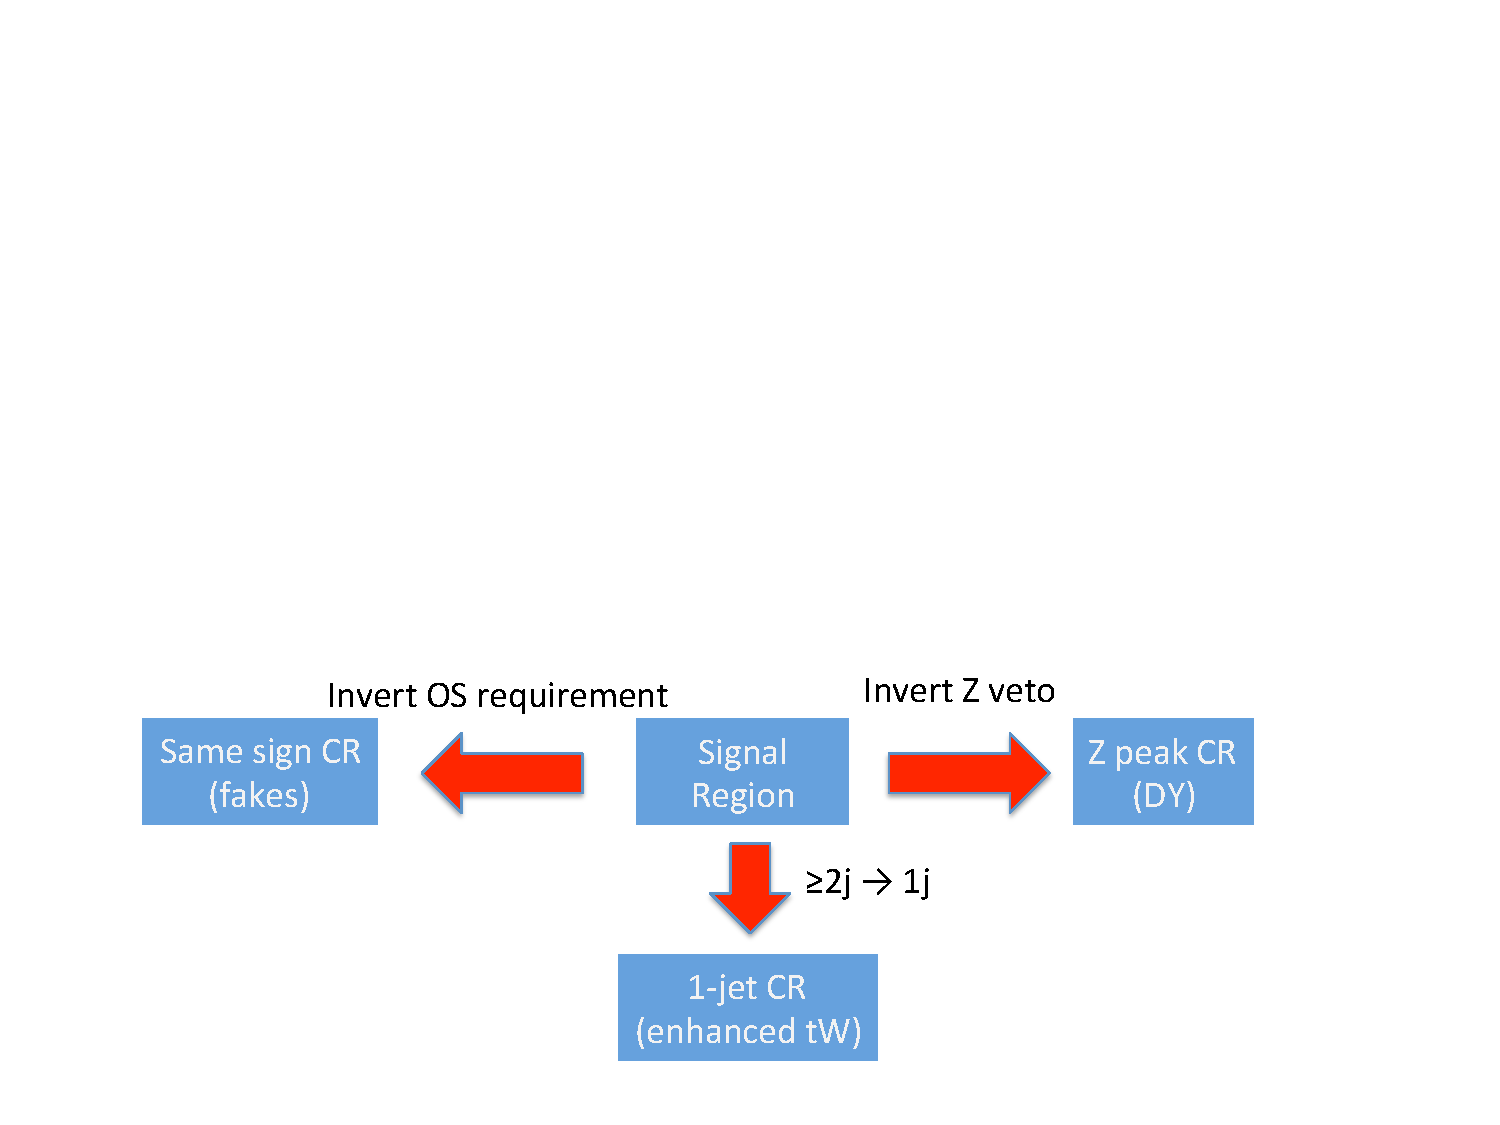
\includegraphics[width=0.75\textwidth]{figures/CRsdef.pdf}
  \caption{Relationships between the SR and the different categories of CRs.}
  \label{fig:afb:crs}
\end{figure}


% Adapted from AN-14-246 UNPUBLISHED! %%%%%%%%%%%%%%%%%%
\begin{table}[h]
\begin{center}
\caption{Summary of control regions. For each ``CR$N$'' other than
  CR0, there is a corresponding ``CR$N$v'', with a b-veto added.}
\label{tab:afb:crdefs}
{\small
\begin{tabular}{l|c c}
\hline
Selection Criteria & Name & Target process  \\
\hline
b veto & CR0 & DY \\
\hline
Z peak & CR1 & DY \\
\hline
Z peak, no MET cut & CR2 & DY \\
\hline
No MET cut & CR3 & DY \\
\hline
1 jet & CR4 & tW  \\
\hline
Same sign & CR5 & Fakes \\
\hline
Same sign, no MET cut & CR6 & Fakes \\
\hline
\end{tabular}
}
\end{center}
\end{table}

In each control region, we vary the normalization of the targeted
background process until the MC yield matches the data yield in that
region. The SF for the DY process is taken from CR1, and the SF for
fakes is taken from CR5; in each case, the related CRs are used to
derive an envelope of variation that defines the systematic
uncertainties on the SFs. These envelopes are depicted in Figure
\ref{fig:afb:sfvariations}, and the final SFs and uncertainties are
given in Table \ref{tab:afb:sfs}. Since CR4 validates the modeling of
the $tW$ background, and thus our decision not to apply a SF, we take
the uncertainty on this background component from a CMS cross section
measurement of $23.4 \pm 5.4$ pb \cite{twxsec}.

There are a few more backgrounds that come from rare processes. These
include $\ttbar$ production in association with a W or Z boson, or a
photon; diboson prorduction (WW, ZZ, WZ); and triboson production
(WWW, WWZ, WZZ, ZZZ). The cross sections for these processes are
extremely small compared to that for $ttdilep$, so we predict them
directly from MC, and assign a 50\% systematic uncertainty. The
background from QCD processes is expected to be negligible, a fact we
verify in a loosened version of CR5.

% Pulled from AN-14-246. UNPUBLISHED! %%%%%%%%%%%%%%%%%
\begin{figure}[t]
  \centering
  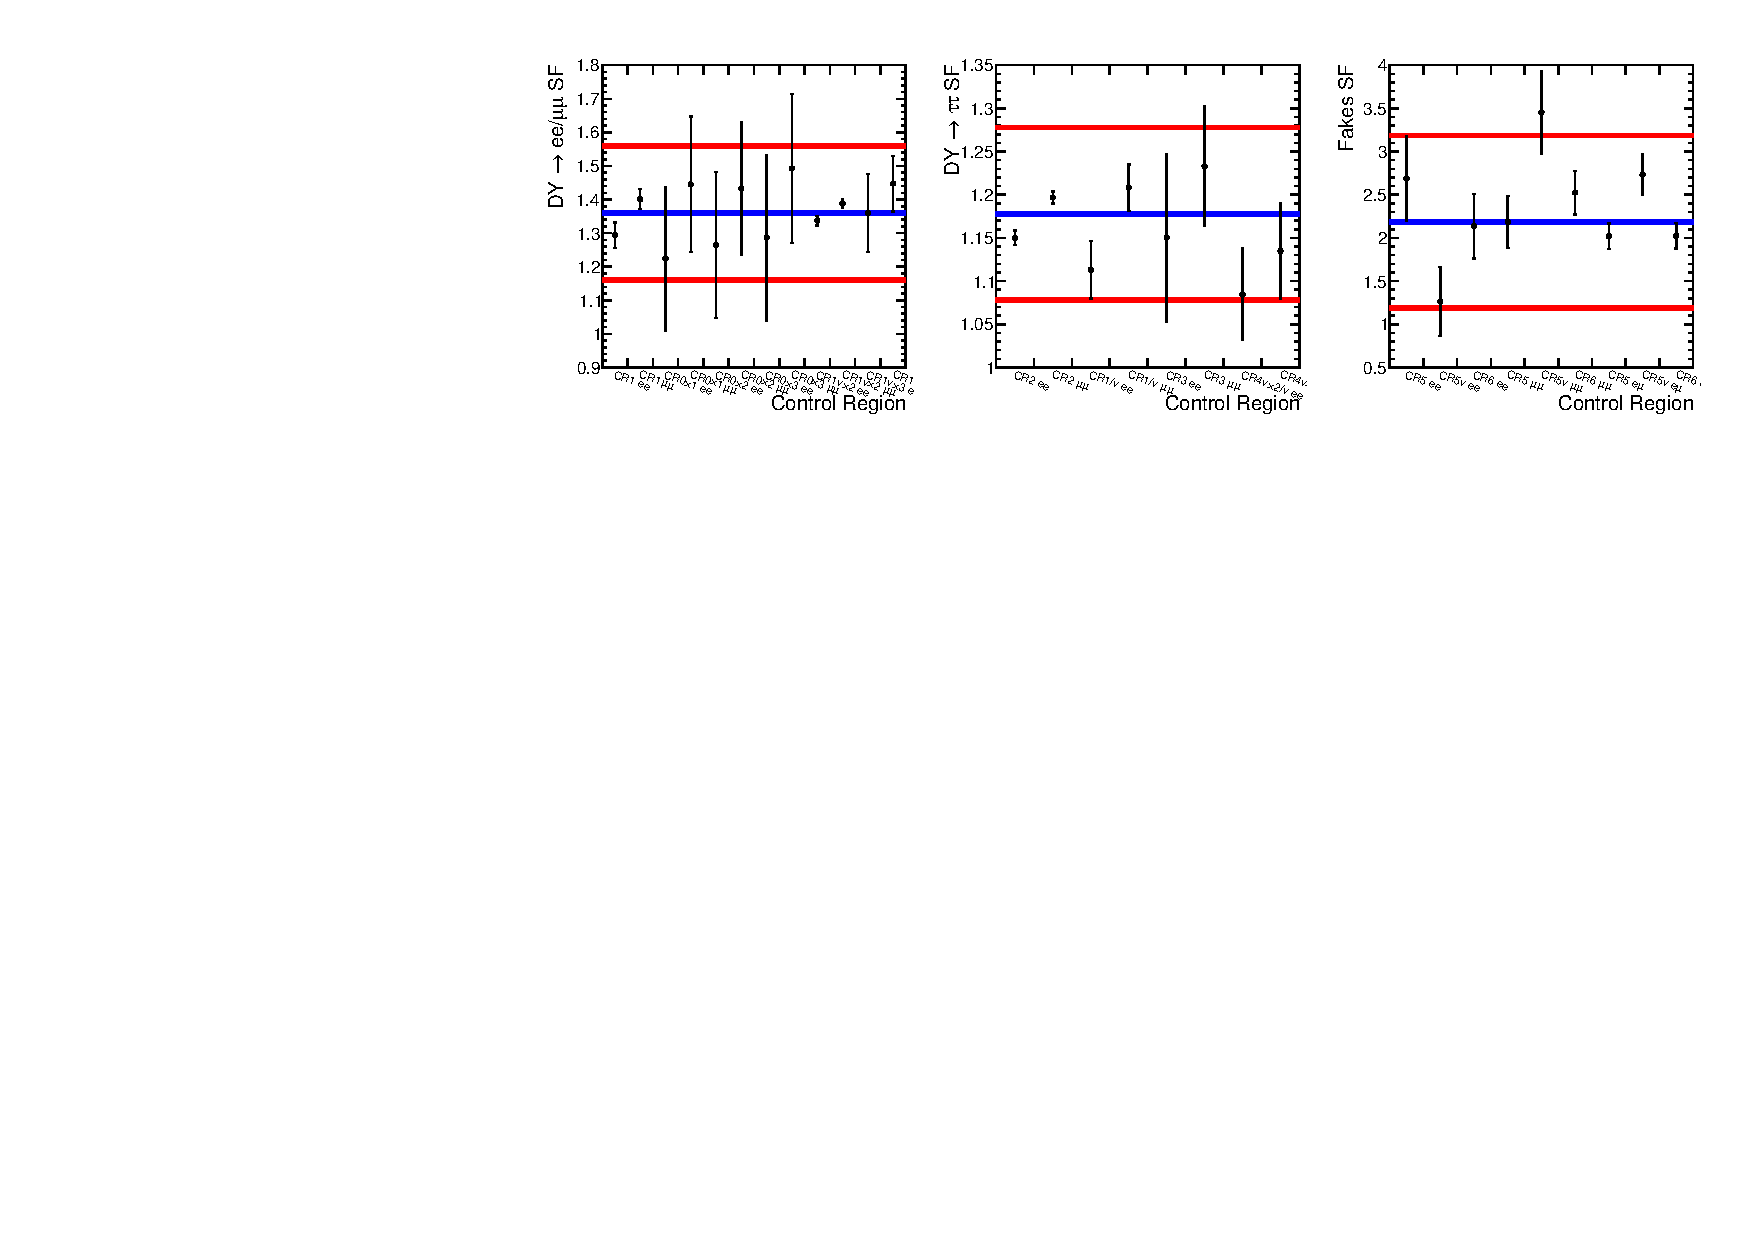
\includegraphics[width=0.75\textwidth]{figures/SFs_all.pdf}
  \caption{SFs measured in different CRs. Blue line depicts the
    central value, and red lines give the systematic uncertainty band.}
  \label{fig:afb:sfvariations}
\end{figure}

% Pulled from AN-14-246. Something similar has been published.
\begin{table}[h]
\begin{center}
\caption{SFs applied to the background components, and their
  associated uncertainties.}
\label{tab:afb:sfs}
{\small
\begin{tabular}{l|c}
\hline
Process & SF  \\
\hline
DY$\rightarrow ee/\mu\mu$ & 1.36 $\pm$ 0.02 (stat) $\pm$ 0.2 (syst) \\
DY$\rightarrow\tau\tau$   & 1.18 $\pm$ 0.01 (stat) $\pm$ 0.1 (syst) \\
fakes             & 2.18 $\pm$ 0.30 (stat) $\pm$ 1.0 (syst) \\
tW                & 1.00 $\pm$ 0.25 (syst) \\
\hline
\end{tabular}
}
\end{center}
\end{table}

\section{Comparison Between Data and Simulation}
\label{sec:afb:datamccompare}

After applying the event selections and scale factors described in the
previous section, our MC-predicted and observed event yields are as
shown in Table \ref{tab:afb:datamcyields}. The dileptonic $\ttbar$
MC has been rescaled so that the total MC yield equals the total data
yield, because we assume that anything that isn't background must be
signal. This $\ttdilep$ sample was generated using \textsc{mc@nlo}, and
required a scale factor of 0.95 to match the data yield. The original
cross section was verified using Powheg. After all scale factors are applied, the
total yield is approximately 91\% signal and 9\% background.

Figure \ref{fig:afb:datamcttvars} provides comparisons between data
and Monte Carlo predictions for several of the observables
that describe the $\ttbar$ system, after all corrections and scale
factors have been applied. Figure \ref{fig:afb:datamcasymvars} gives
the same comparisons for the variables used to calculate our asymmetries.
As the plots themselves and the associated
ratios show, the MC predictions match the data fairly well, indicating
good quality modeling of the background processes and the
$\ttdilep$ process.
% Would be nice to stick in a table with the reco-level asymmetries,
% if I could get one where A_P isn't separated by lepton charge...

% Adapted from AN-14-246. Similar table published in spin correlation/polarization paper.
\begin{table}[hbt]
\begin{center}
\caption{Observed and expected yields after applying preselection and scale
  factors. Yields are scaled to a luminosity of 19.5
  fb\textsuperscript{-1}. Uncertainties are statistical only.}
\label{tab:afb:datamcyields}
\begin{tabular}{l |  c  c  c  c}
\hline
                                        Sample   &                $ee$   &            $\mu\mu$   &              $e\mu$   &               Total  \\
\hline
                 $\ttbar \rightarrow \ell\ell$   &   6313.6 $\pm$ 37.7   &   8975.7 $\pm$ 44.1   &  24651.6 $\pm$ 73.4   &  39940.9 $\pm$ 93.6  \\
              $\ttbar \rightarrow \ell +$ jets   &     107.1 $\pm$ 7.7   &      62.2 $\pm$ 5.4   &    327.4 $\pm$ 13.4   &    496.7 $\pm$ 16.4  \\
                                        W+jets   &       7.3 $\pm$ 3.6   &       1.8 $\pm$ 1.8   &      10.0 $\pm$ 3.5   &      19.1 $\pm$ 5.3  \\
                  single top (s/t-chan, 1-lep)   &       2.6 $\pm$ 0.6   &       4.6 $\pm$ 0.9   &      18.8 $\pm$ 1.6   &      26.1 $\pm$ 1.9  \\
                        single top (tW, 2-lep)   &     298.0 $\pm$ 1.6   &     425.9 $\pm$ 1.9   &    1161.9 $\pm$ 3.1   &    1885.8 $\pm$ 4.0  \\
                                      WW/WZ/ZZ   &      27.6 $\pm$ 1.4   &      40.7 $\pm$ 1.4   &      89.3 $\pm$ 2.3   &     157.5 $\pm$ 3.0  \\
               DY $\rightarrow ee/\mu\mu$+jets   &    211.0 $\pm$ 16.0   &    368.0 $\pm$ 22.8   &       1.6 $\pm$ 0.5   &    580.6 $\pm$ 27.9  \\
                DY $\rightarrow \tau\tau$+jets   &      33.9 $\pm$ 2.5   &      51.5 $\pm$ 3.0   &     137.6 $\pm$ 5.1   &     223.0 $\pm$ 6.4  \\
                                ttW/Z/$\gamma$   &      86.4 $\pm$ 6.5   &     141.3 $\pm$ 8.2   &    331.6 $\pm$ 12.8   &    559.2 $\pm$ 16.5  \\
                                      triboson   &       1.5 $\pm$ 0.1   &       2.3 $\pm$ 0.2   &       5.2 $\pm$ 0.3   &       9.0 $\pm$ 0.4  \\
\hline
                                   Total SM MC   &   7089.0 $\pm$ 42.5   &  10074.0 $\pm$ 50.8   &  26735.0 $\pm$ 76.1   & 43898.0 $\pm$ 100.9  \\
\hline
                                          Data   &                7089   &               10074   &               26735   &               43898  \\
\hline

\end{tabular}
\end{center}
\end{table}

% Pulled from AN-14-246. Some of these plots are published in the spin corr/pol paper, and in supplementary material in the charge asym paper.
\begin{figure}[phtb]
  \centering
  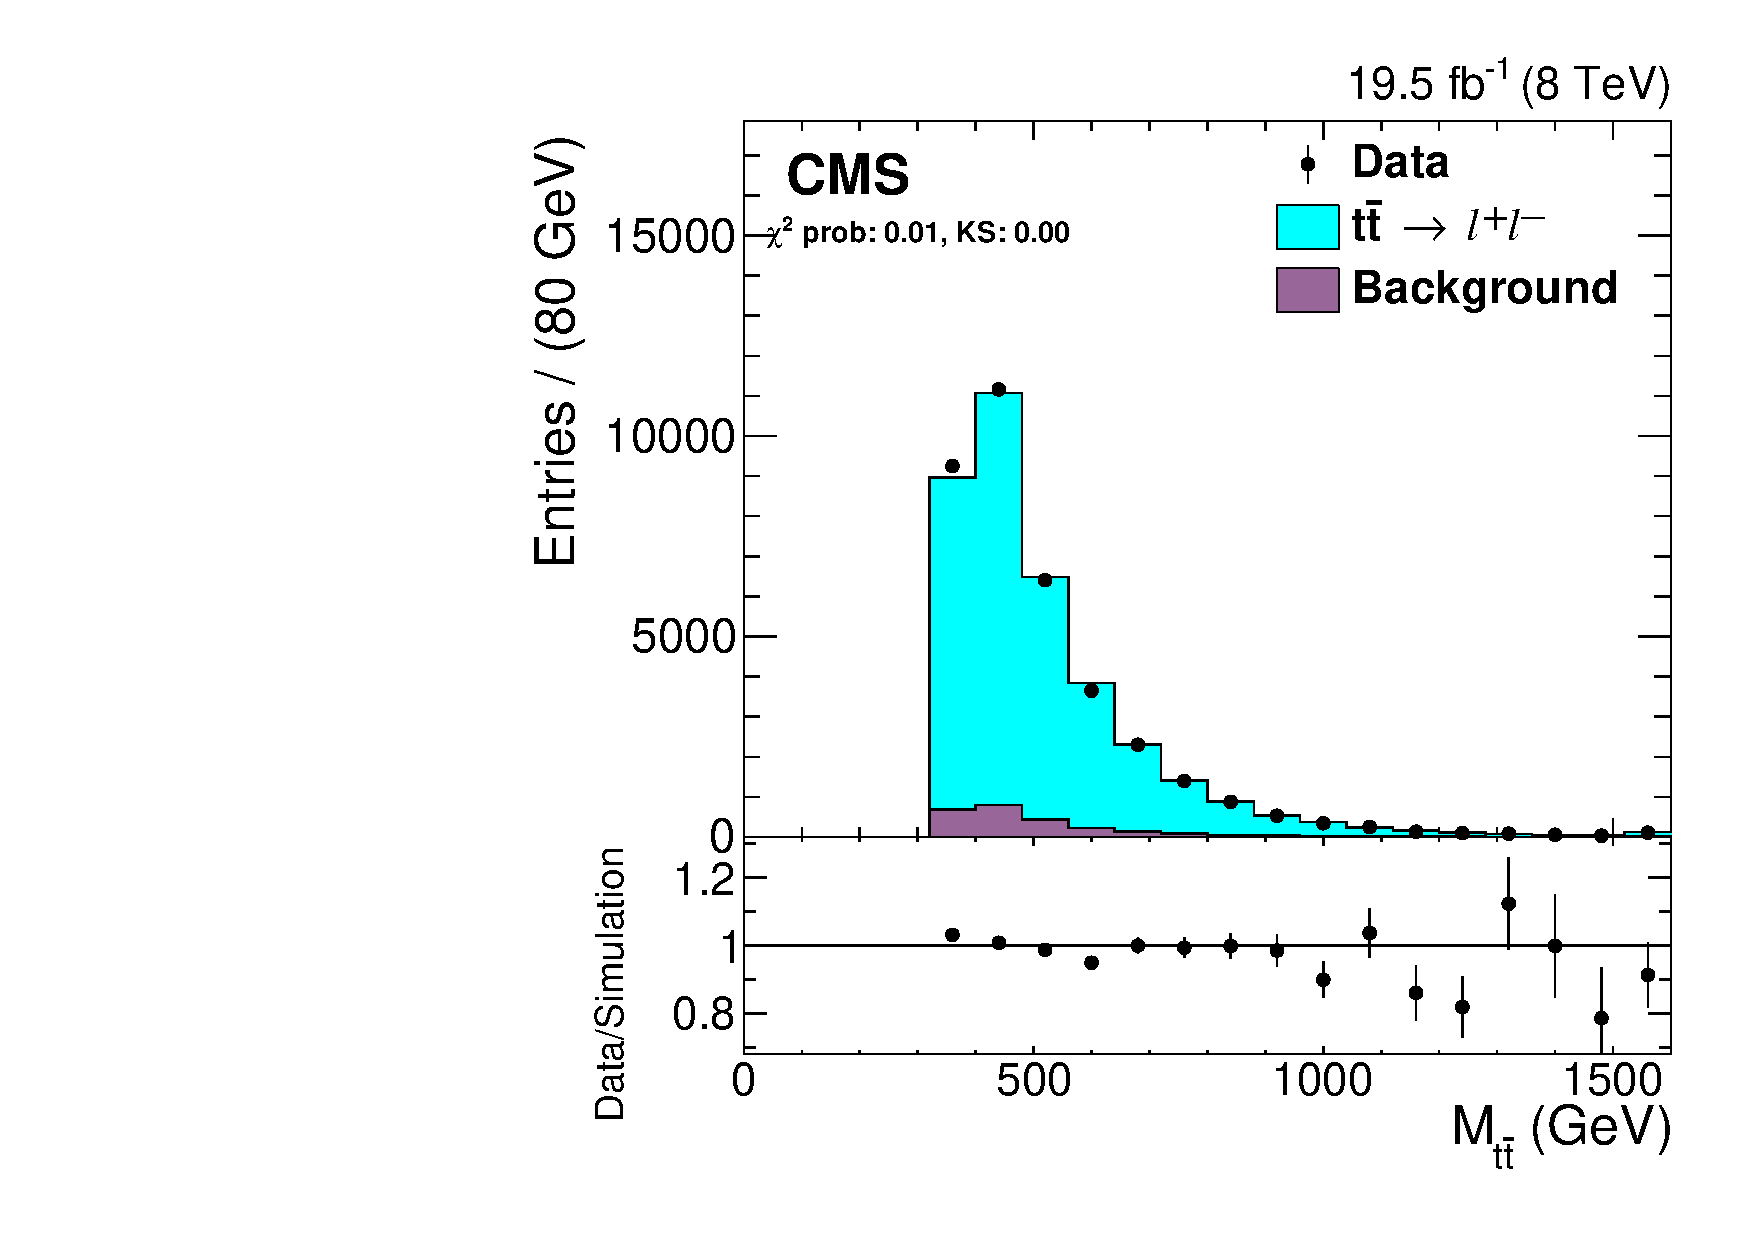
\includegraphics[width=0.325\textwidth]{figures/dataMC_ttmass.pdf}
  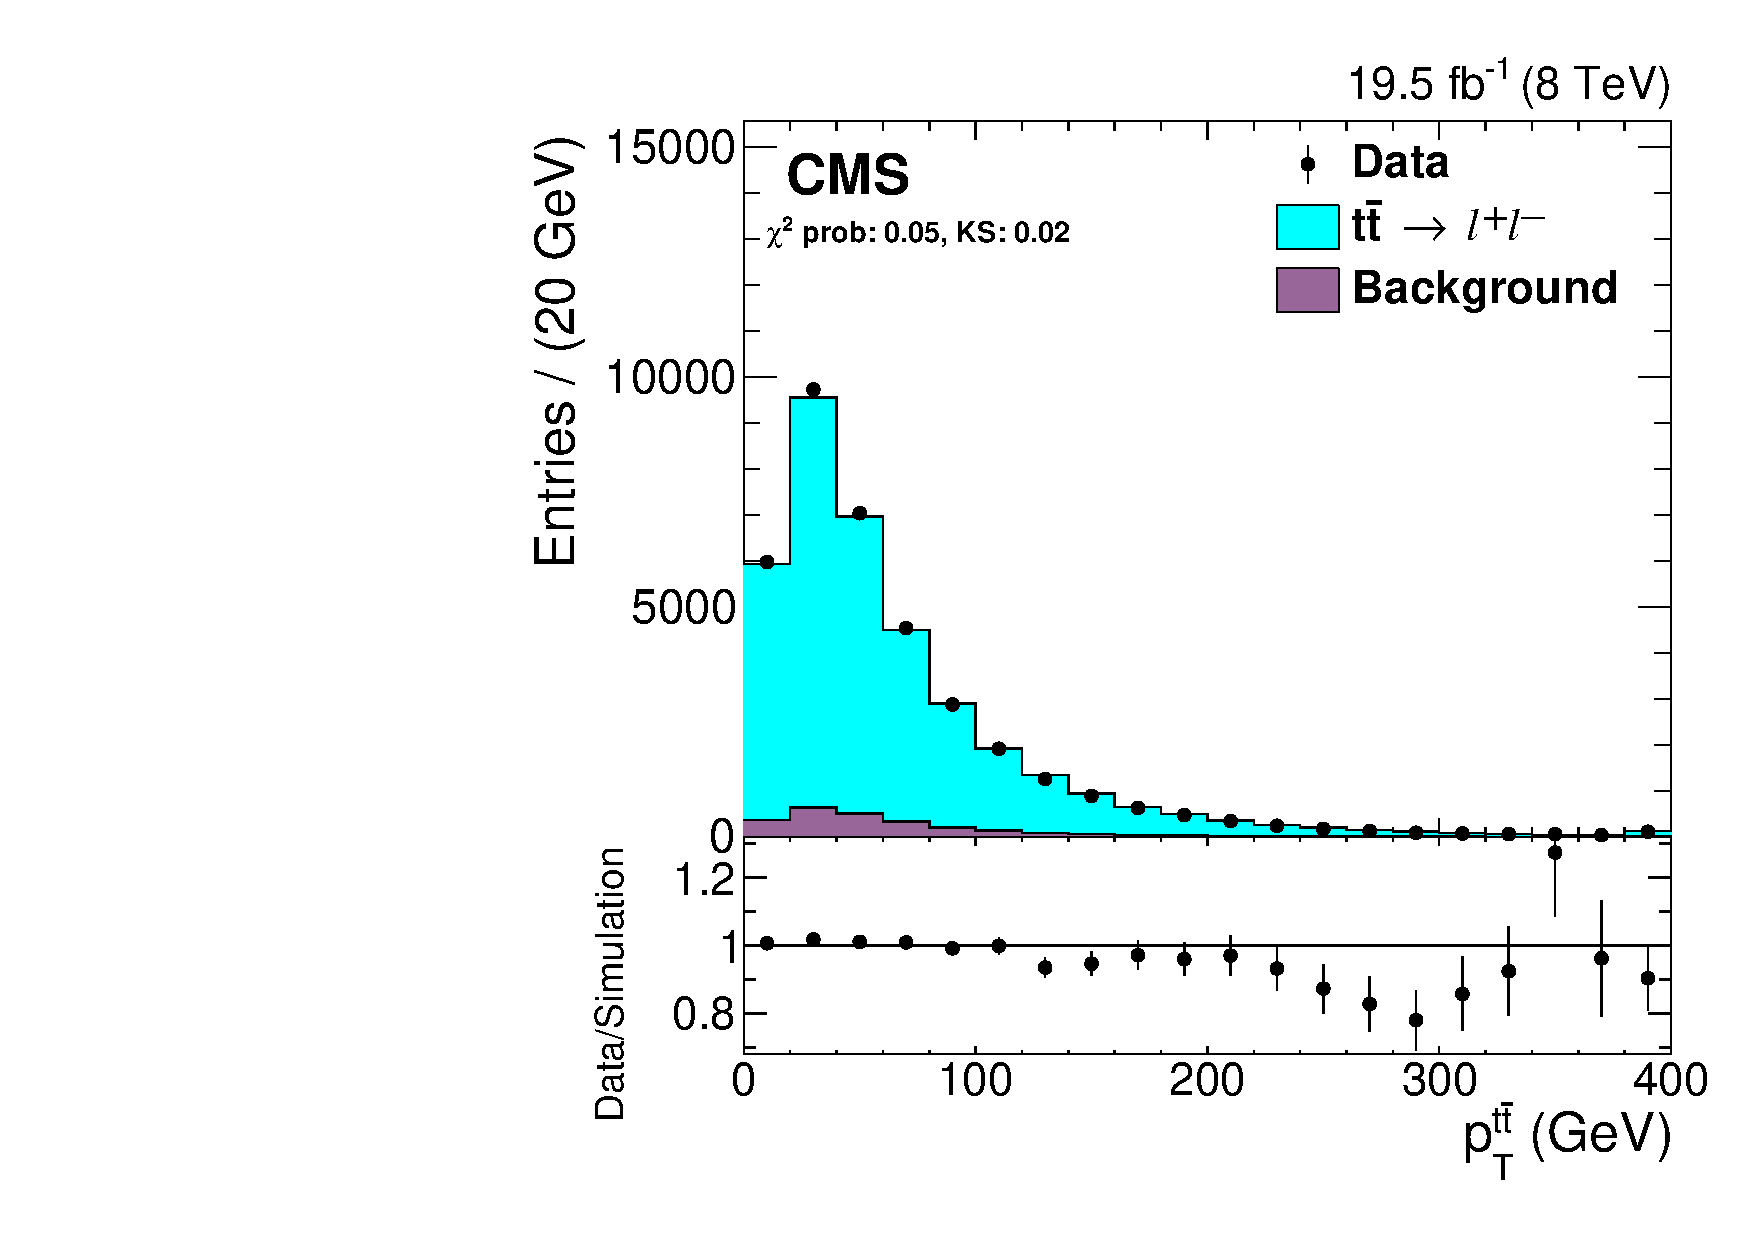
\includegraphics[width=0.325\textwidth]{figures/dataMC_ttpT.pdf}
  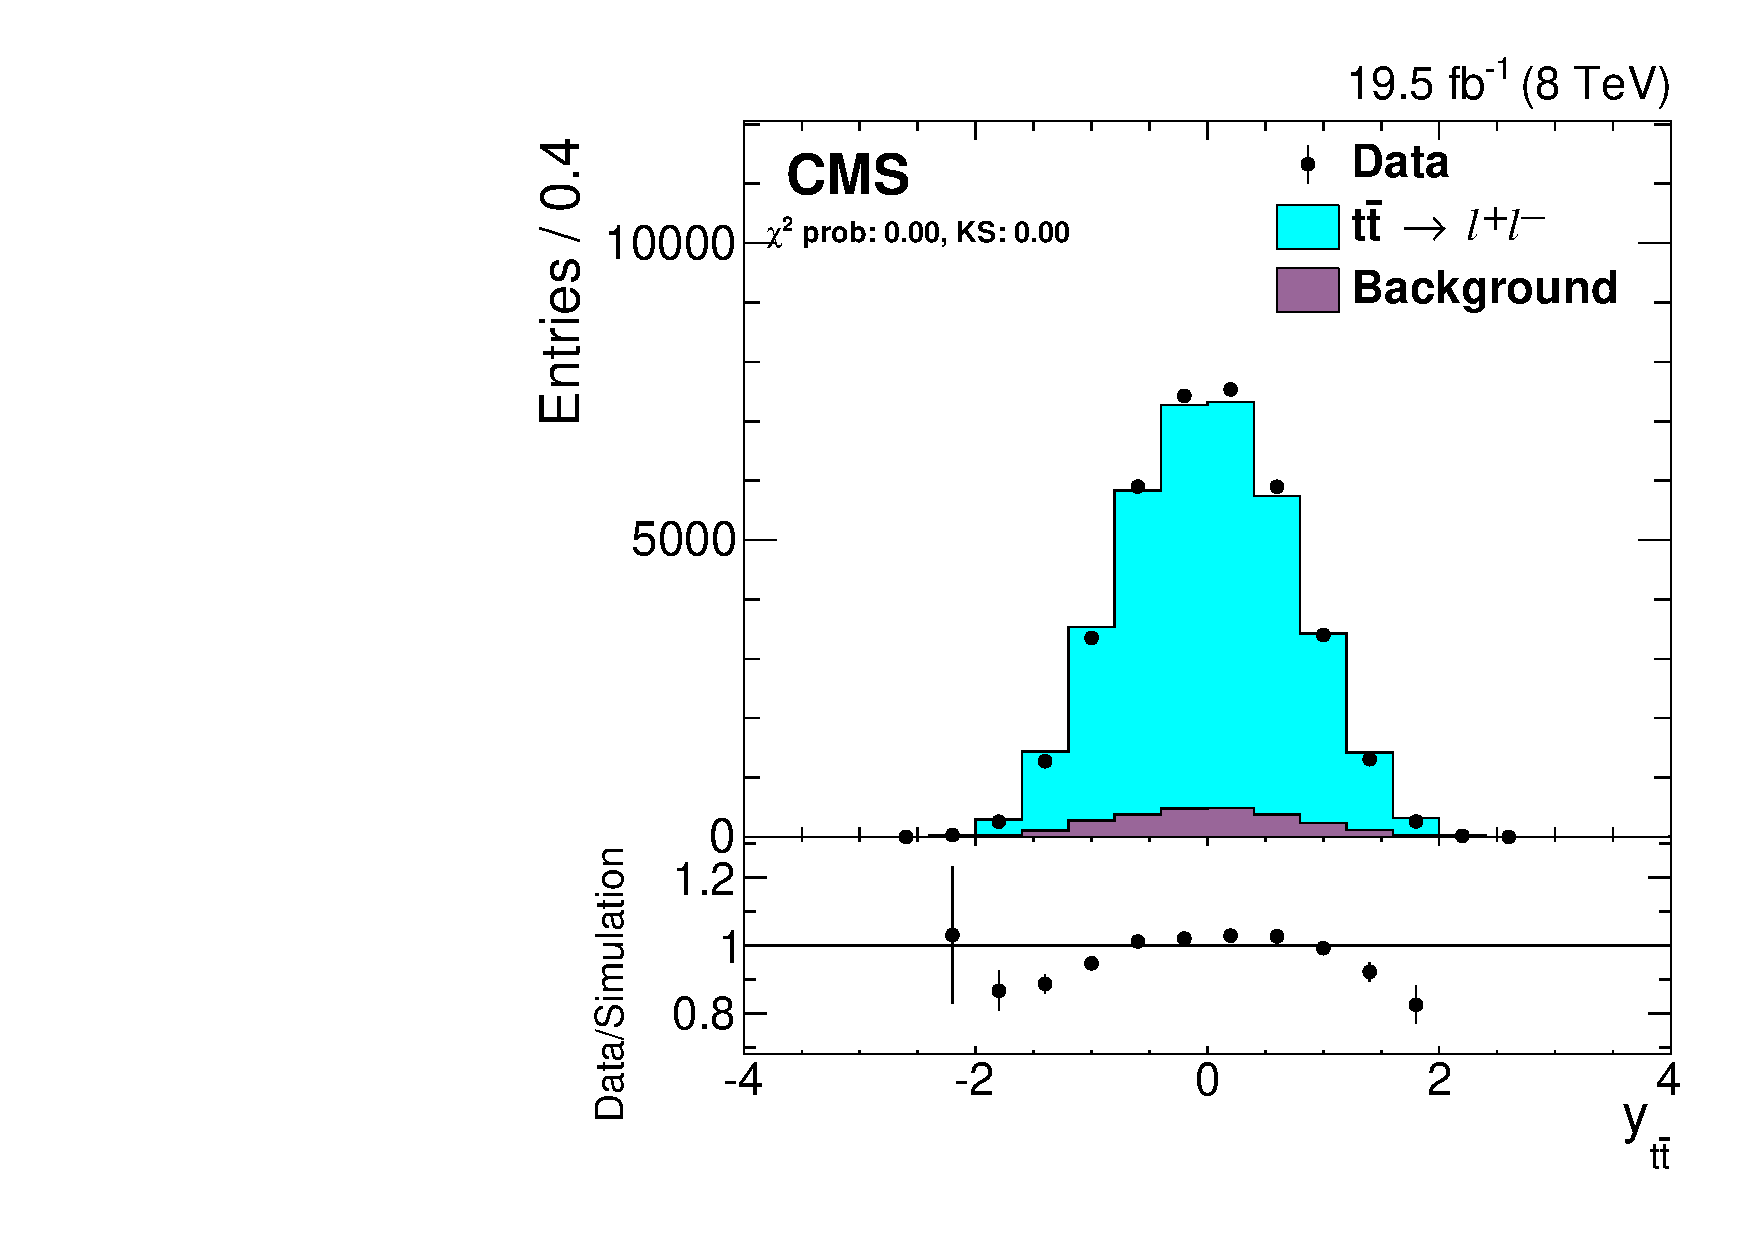
\includegraphics[width=0.325\textwidth]{figures/dataMC_ttRapidity2.pdf}
  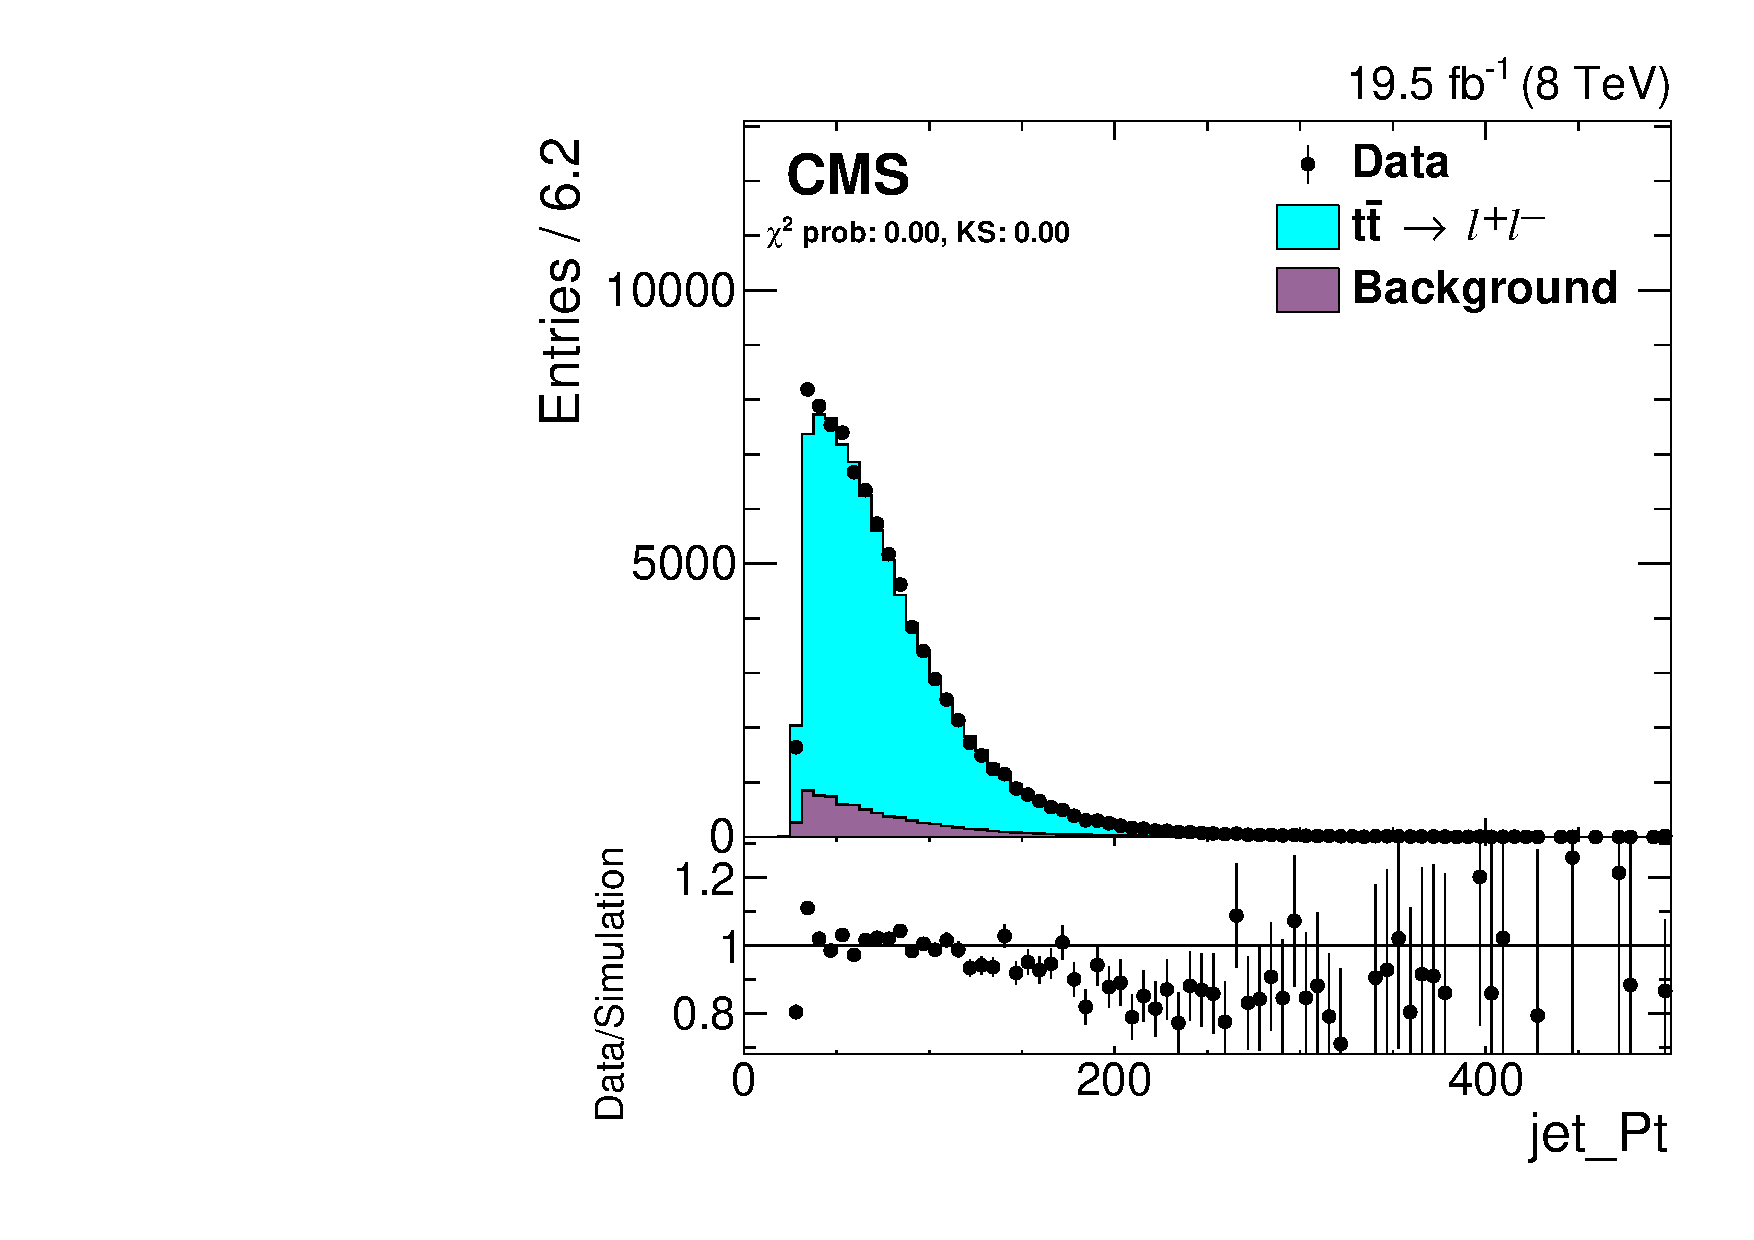
\includegraphics[width=0.325\textwidth]{figures/dataMC_jetpT.pdf}
  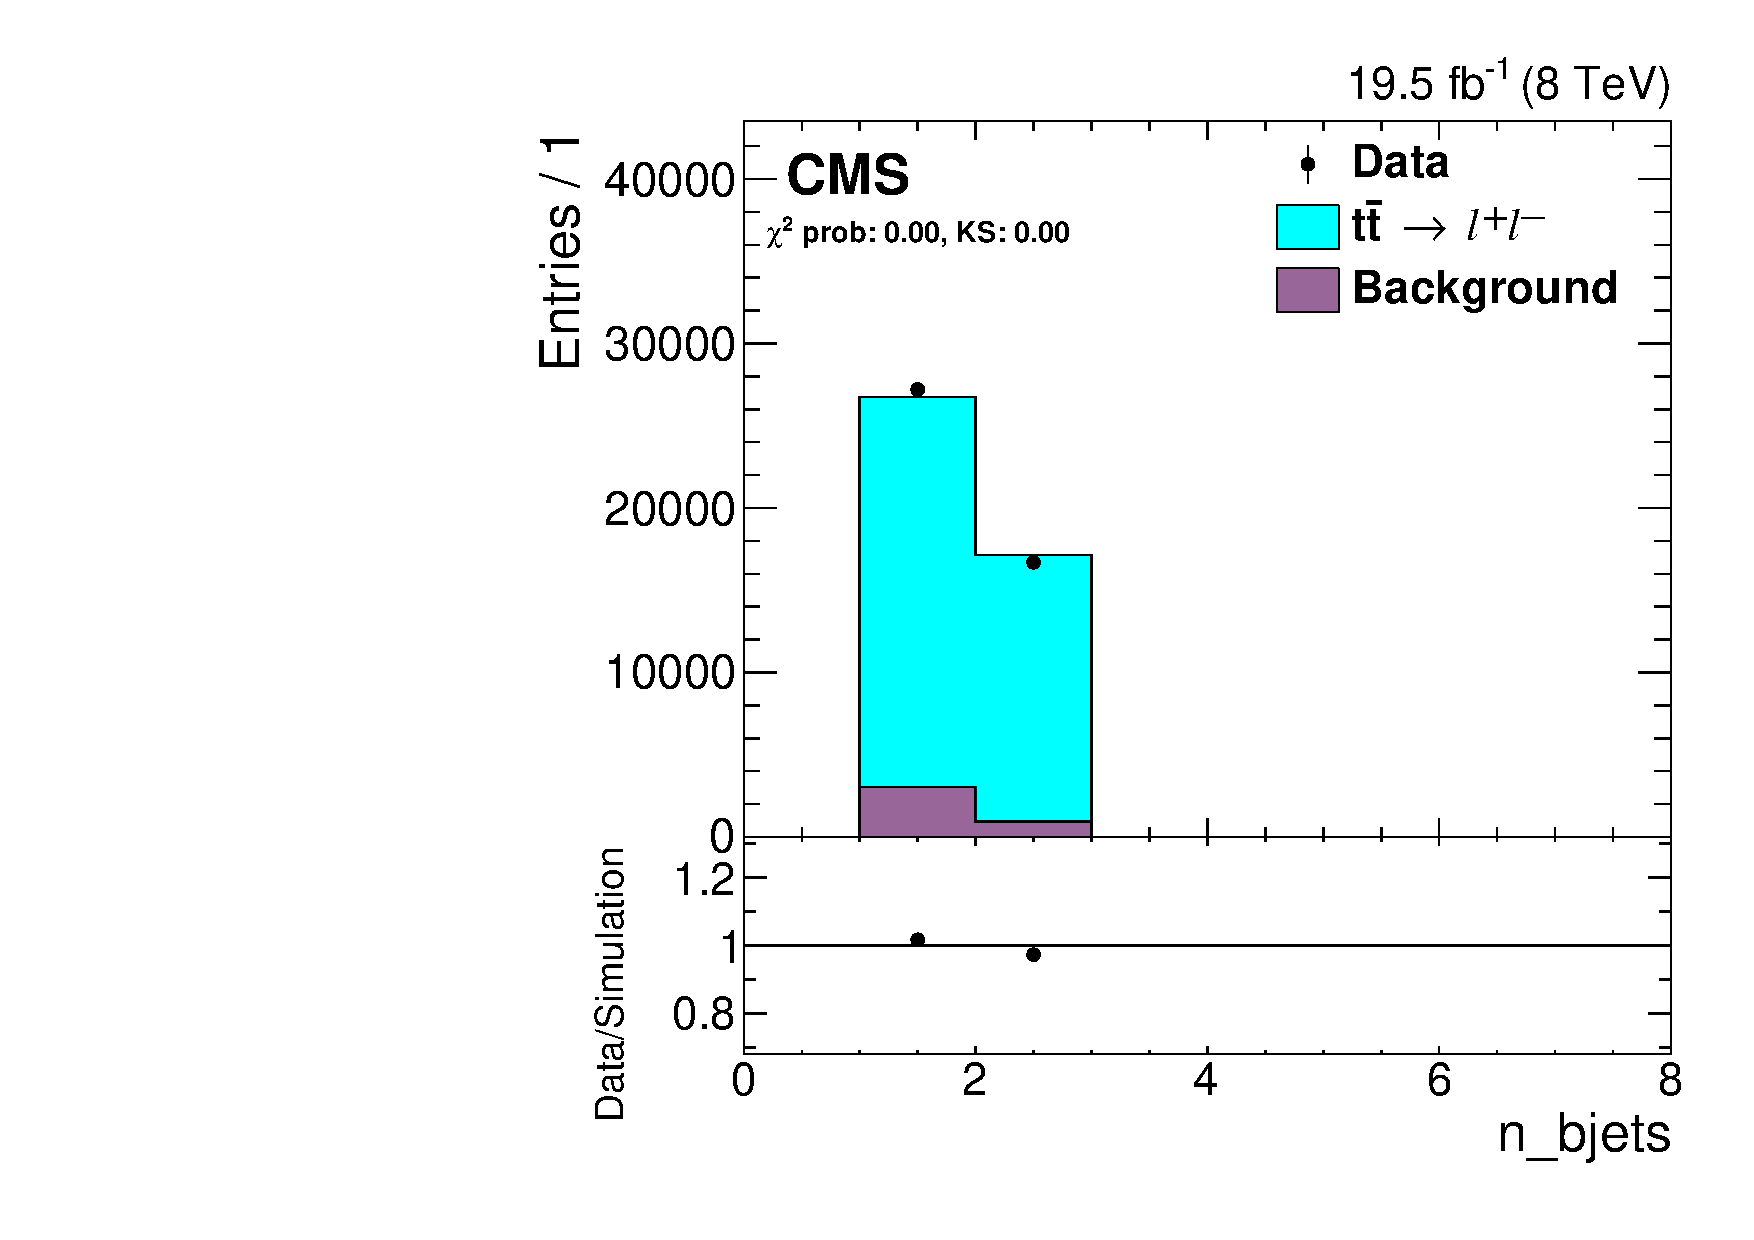
\includegraphics[width=0.325\textwidth]{figures/dataMC_nbjets.pdf}
  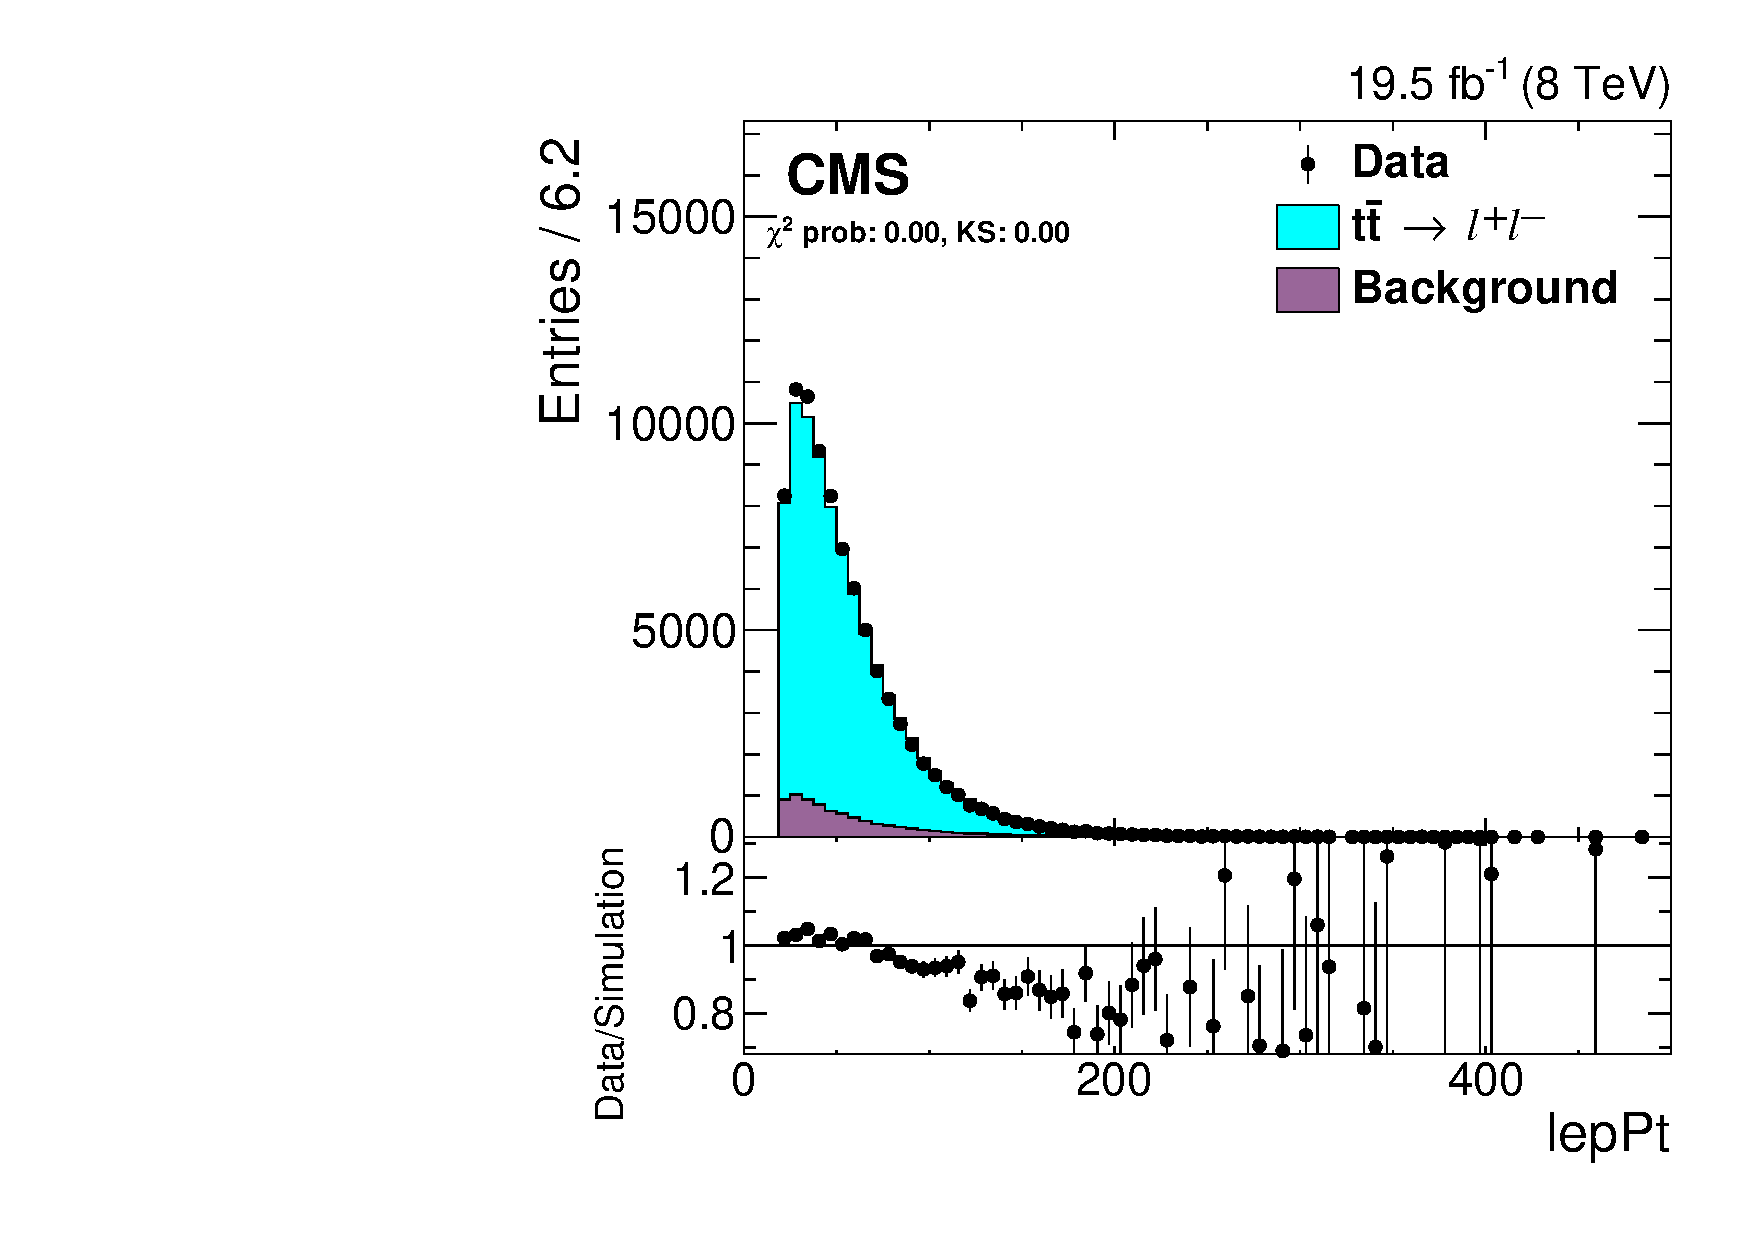
\includegraphics[width=0.325\textwidth]{figures/dataMC_lepPt.pdf}
  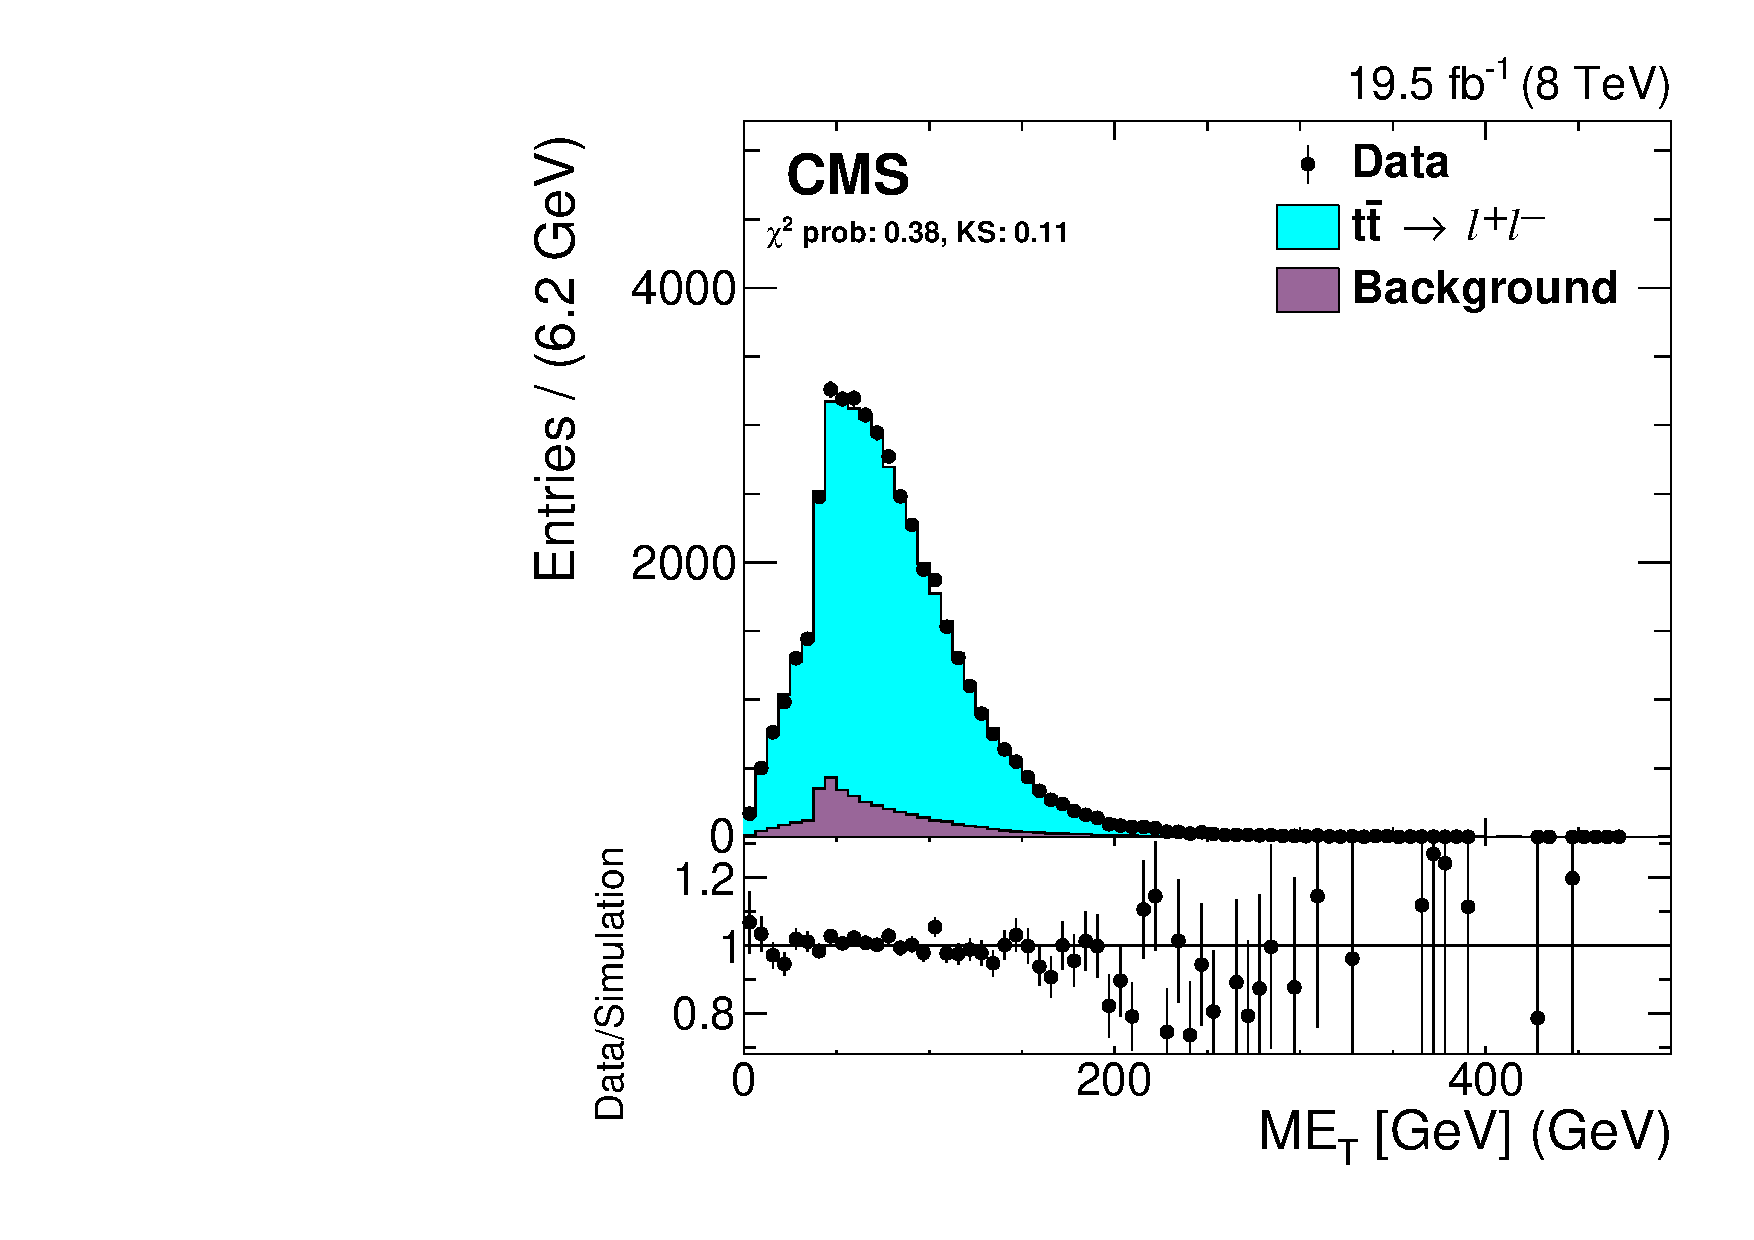
\includegraphics[width=0.325\textwidth]{figures/dataMC_met.pdf}
  \caption{Comparison of data with Monte Carlo predictions for
    selected $\ttbar$ observables.}
  \label{fig:afb:datamcttvars}
\end{figure}
% Are there any other plots that are important to show good modeling?

\begin{figure}[phtb]
  \centering
  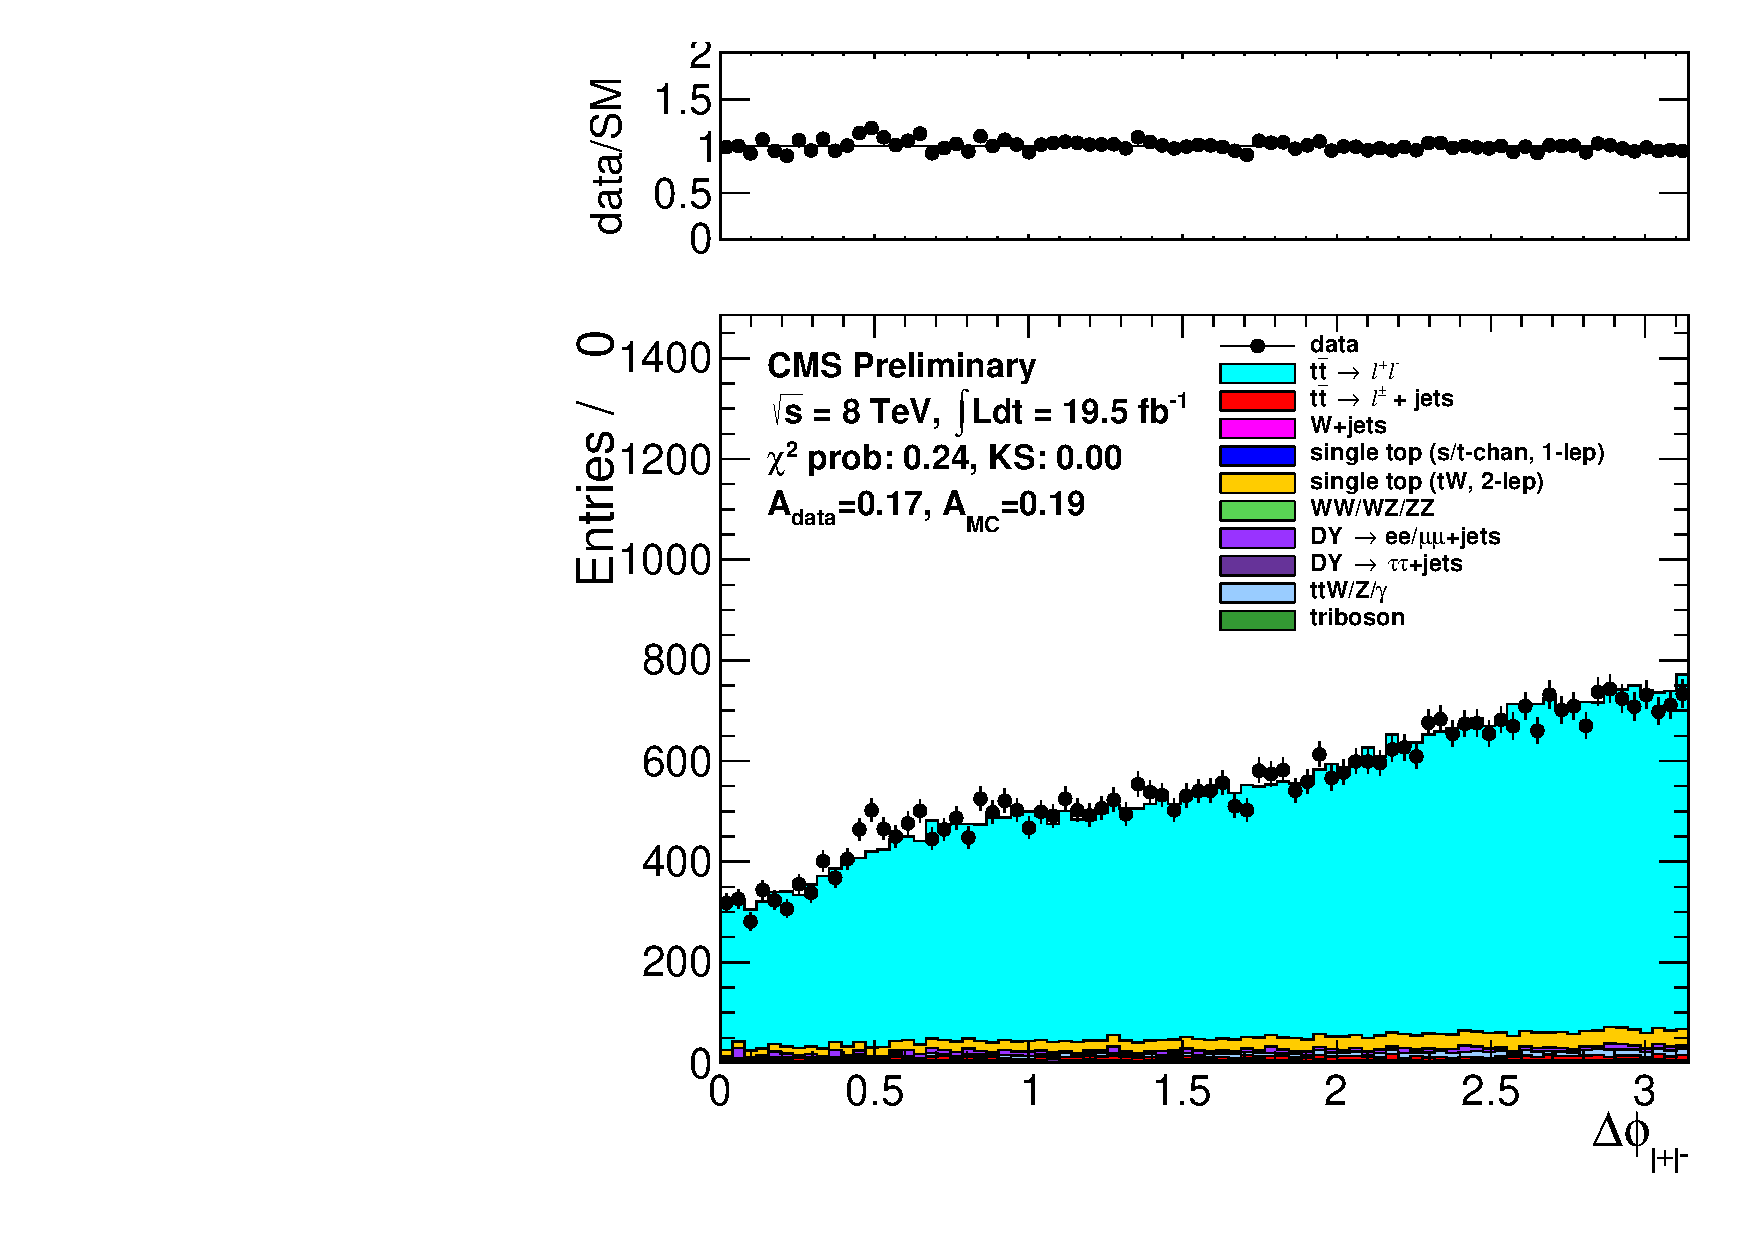
\includegraphics[width=0.325\textwidth]{figures/dataMC_lep_azimuthal_asymmetry2_combined.pdf}
  % 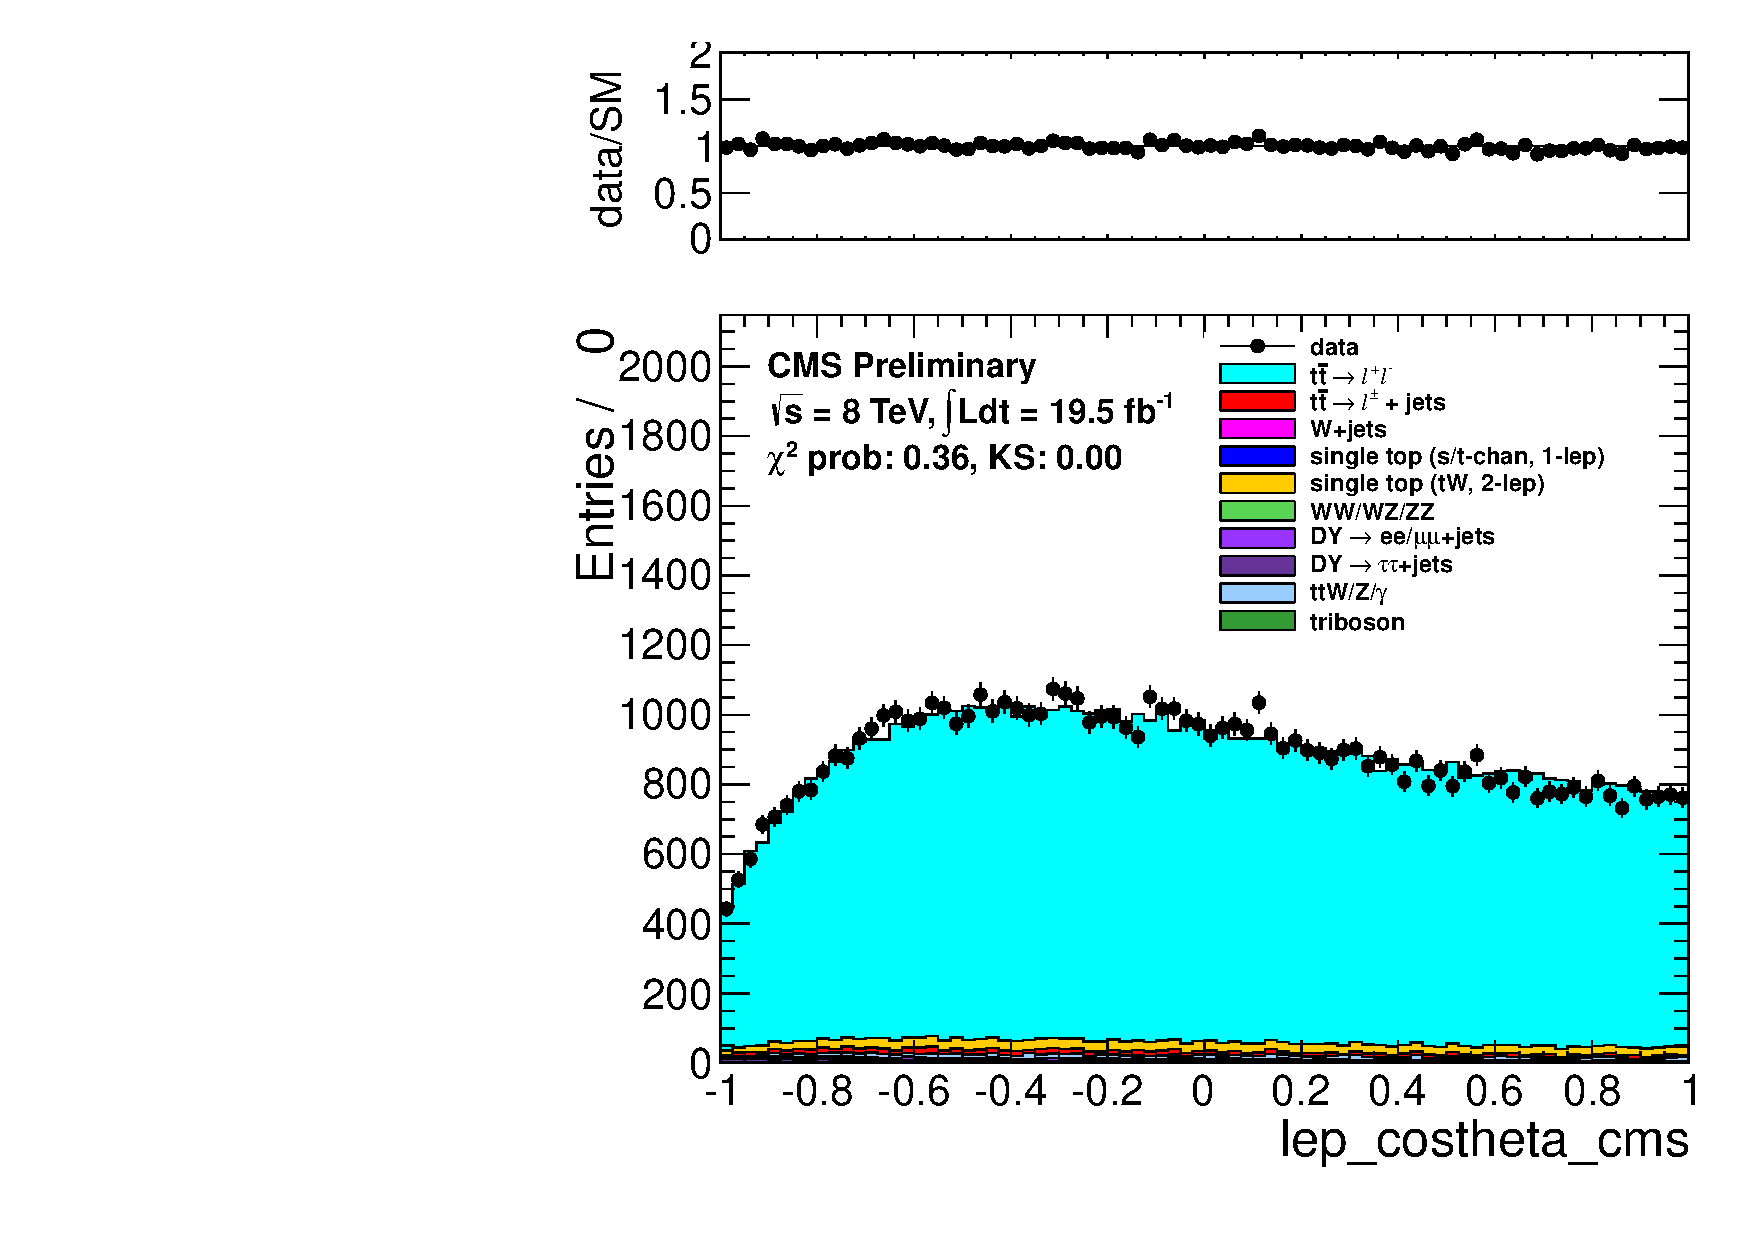
\includegraphics[width=0.45\textwidth]{figures/dataMC_lep_costheta_combined} % Unofficial plot
  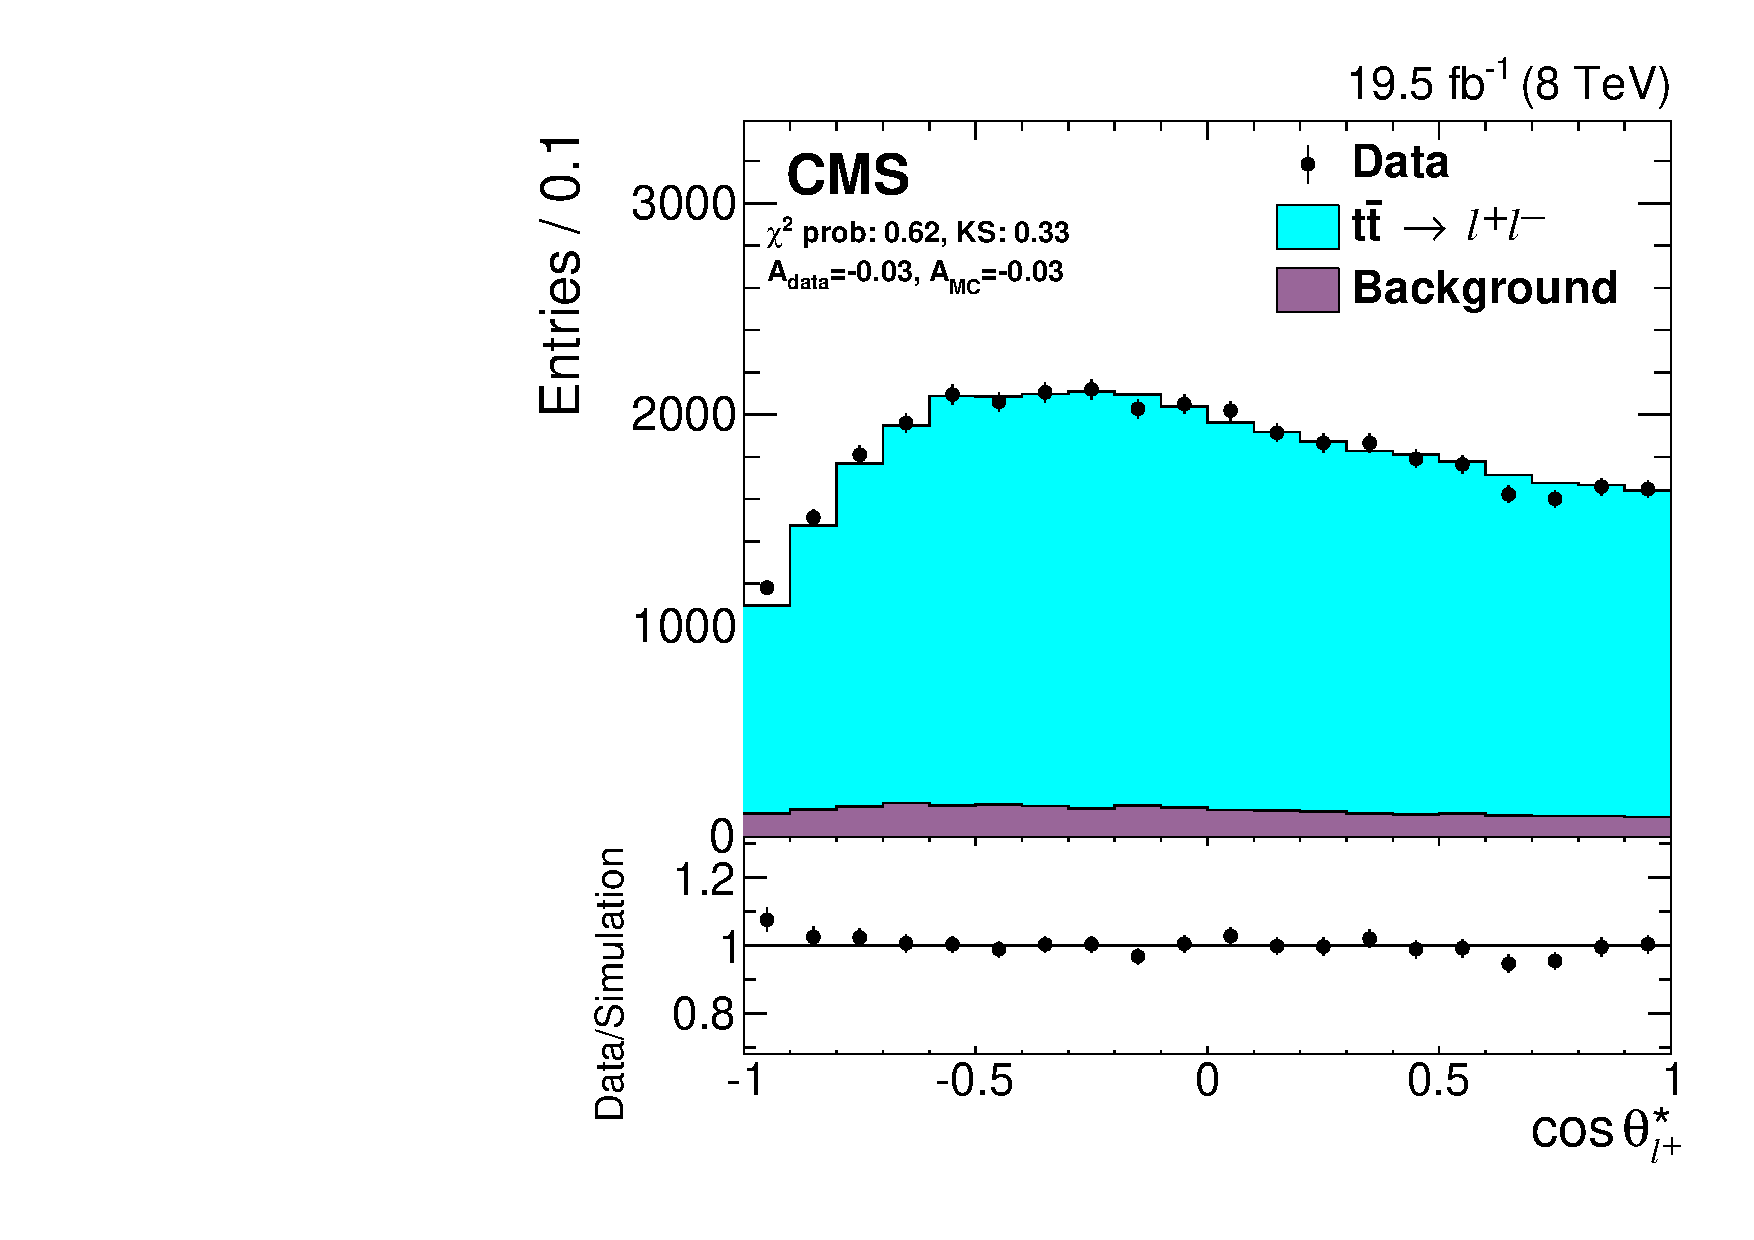
\includegraphics[width=0.325\textwidth]{figures/dataMC_lepPlus_costheta_cms_combined.pdf}
  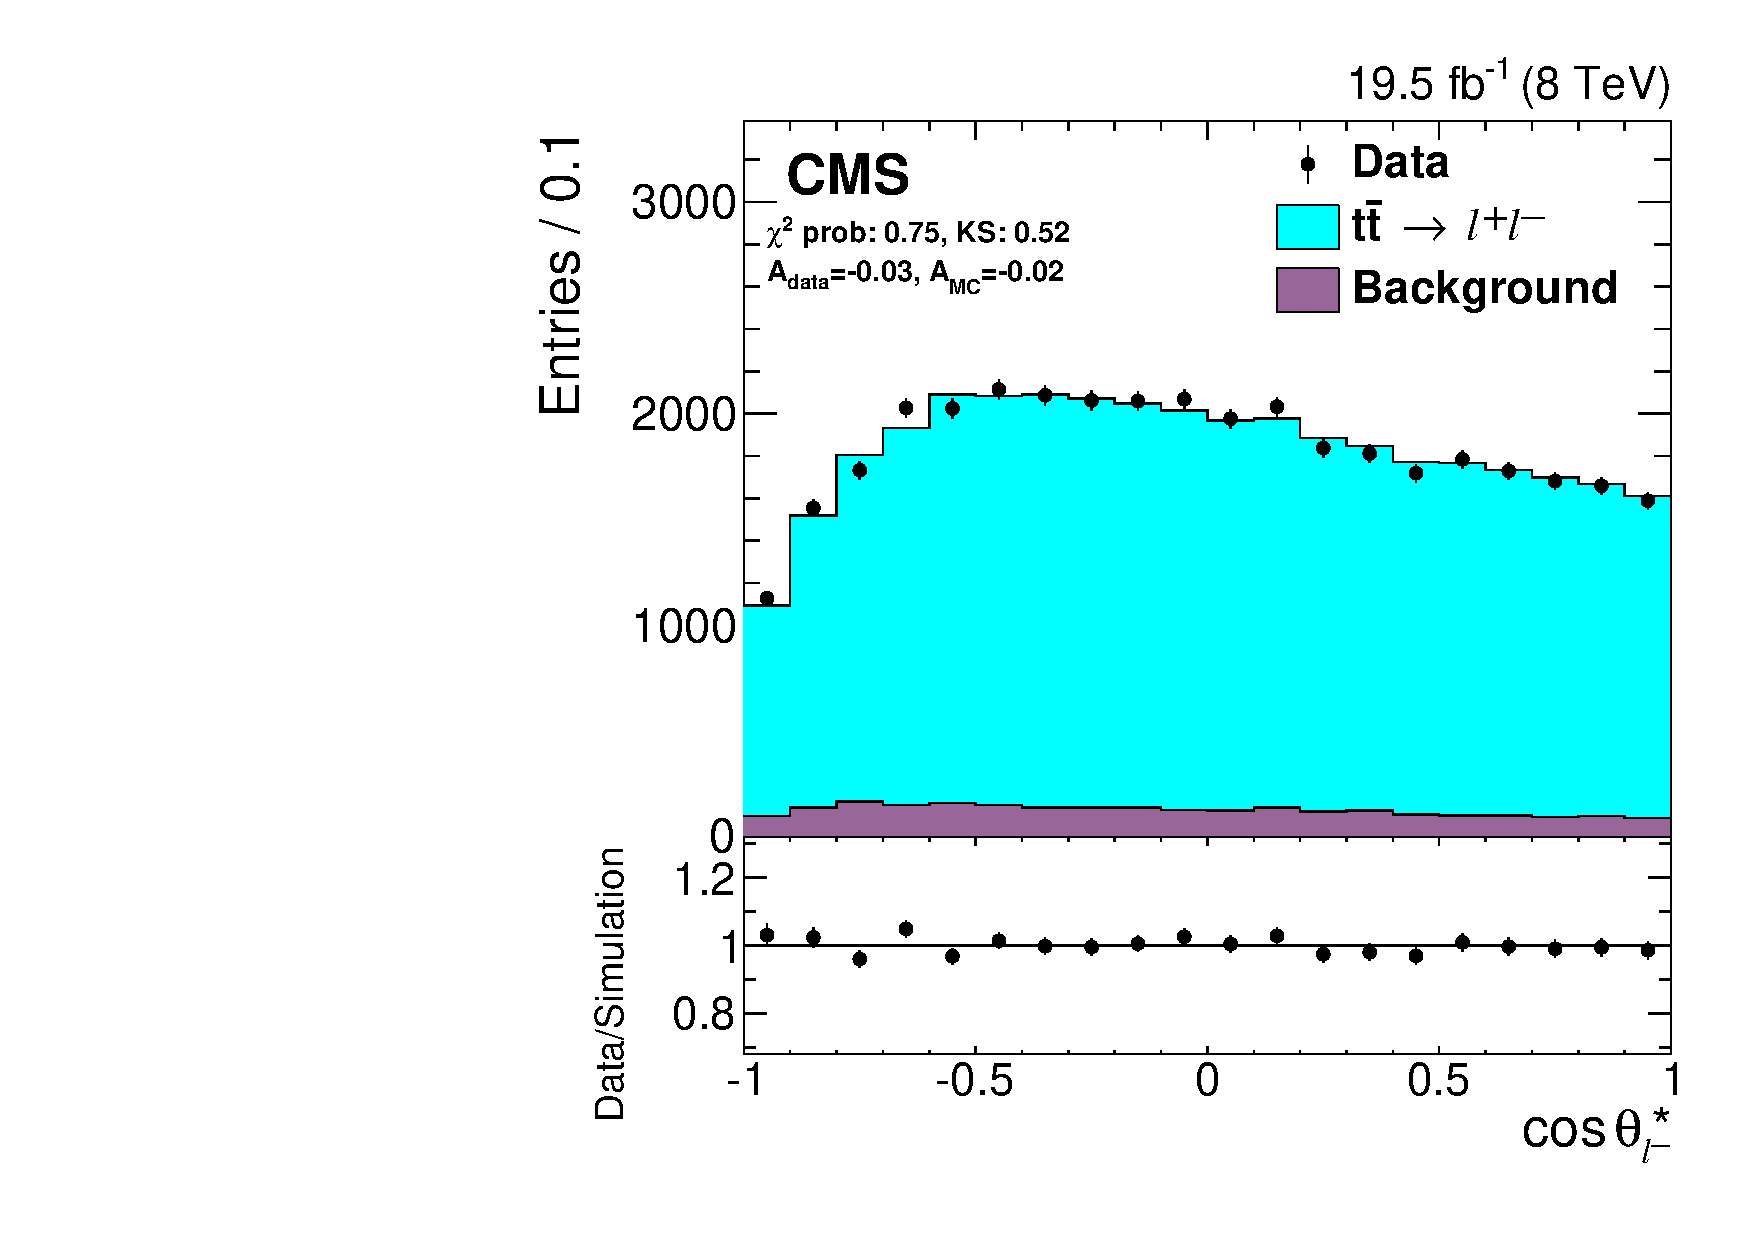
\includegraphics[width=0.325\textwidth]{figures/dataMC_lepMinus_costheta_cms_combined.pdf}
  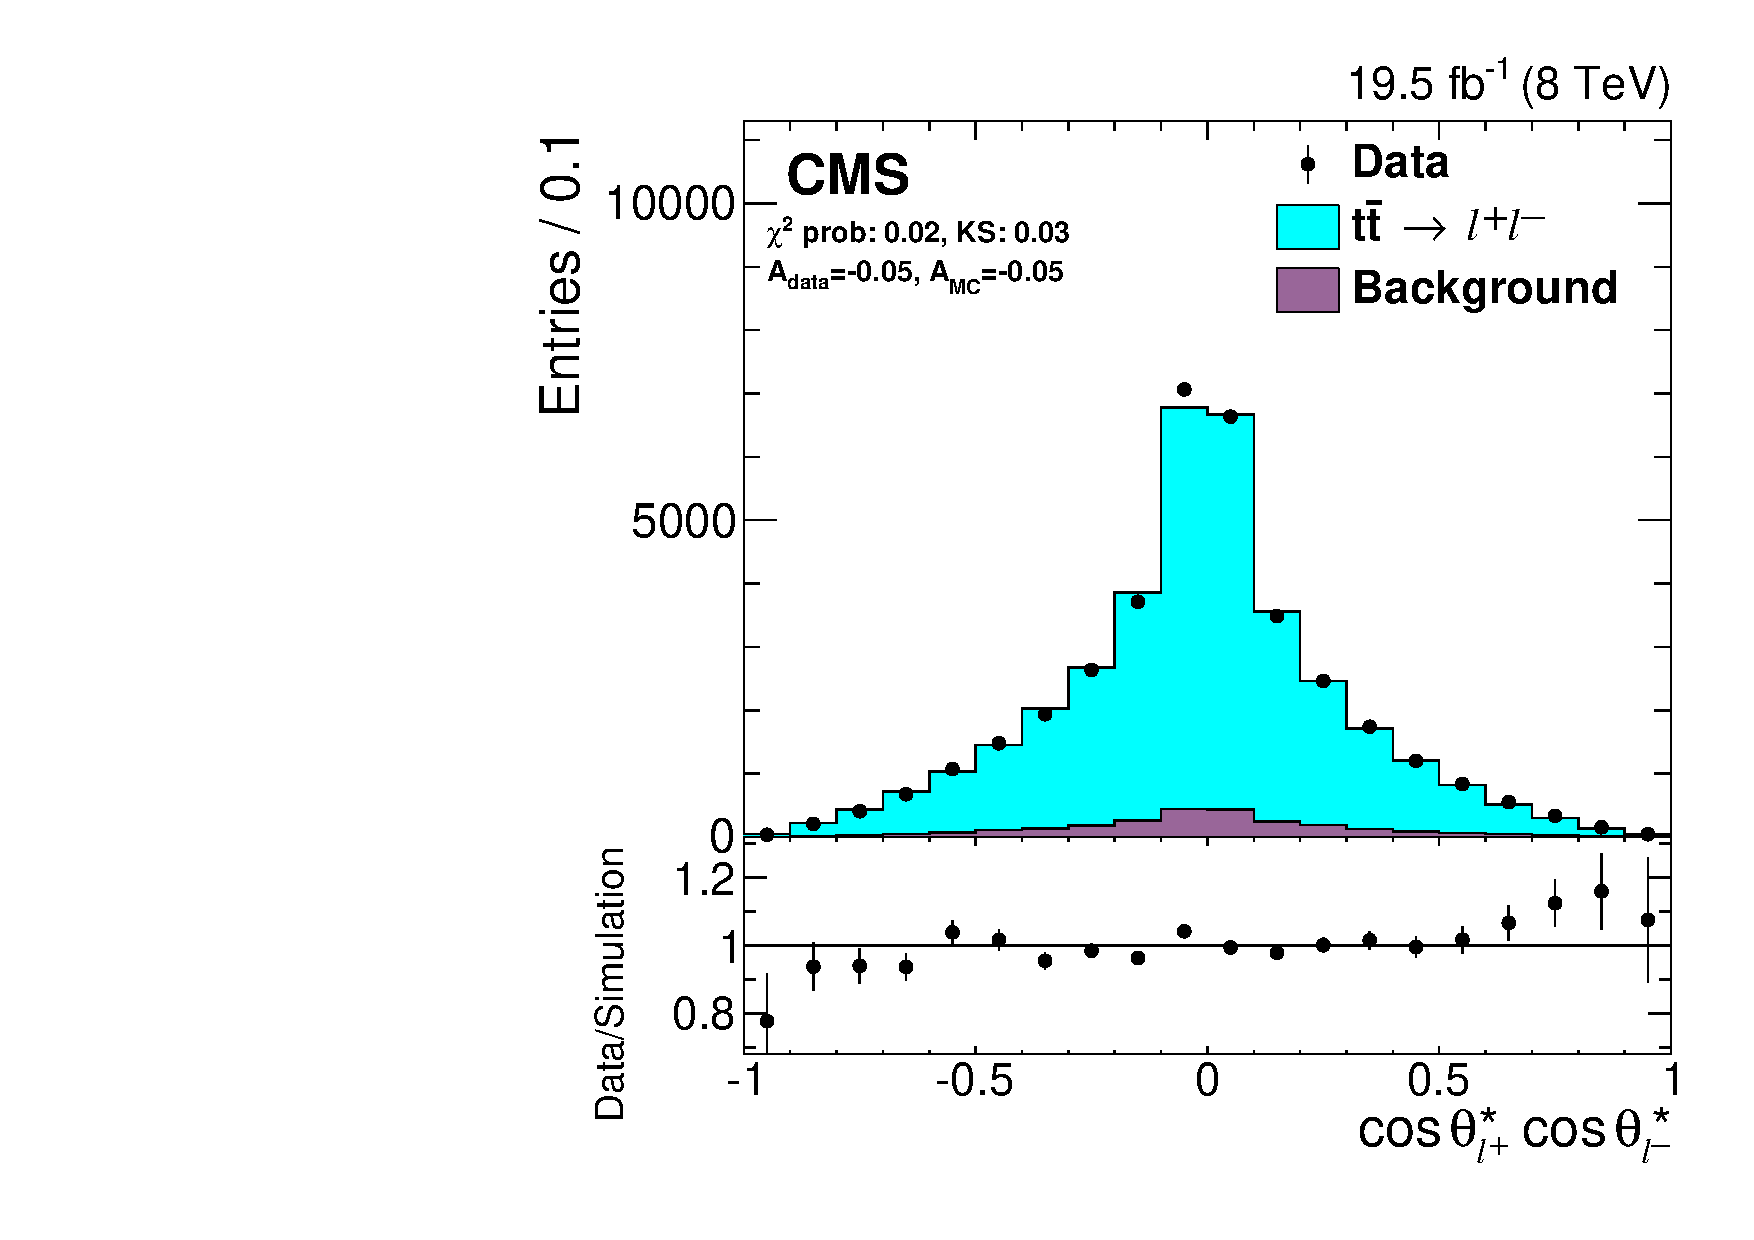
\includegraphics[width=0.325\textwidth]{figures/dataMC_top_spin_correlation_combined.pdf}
  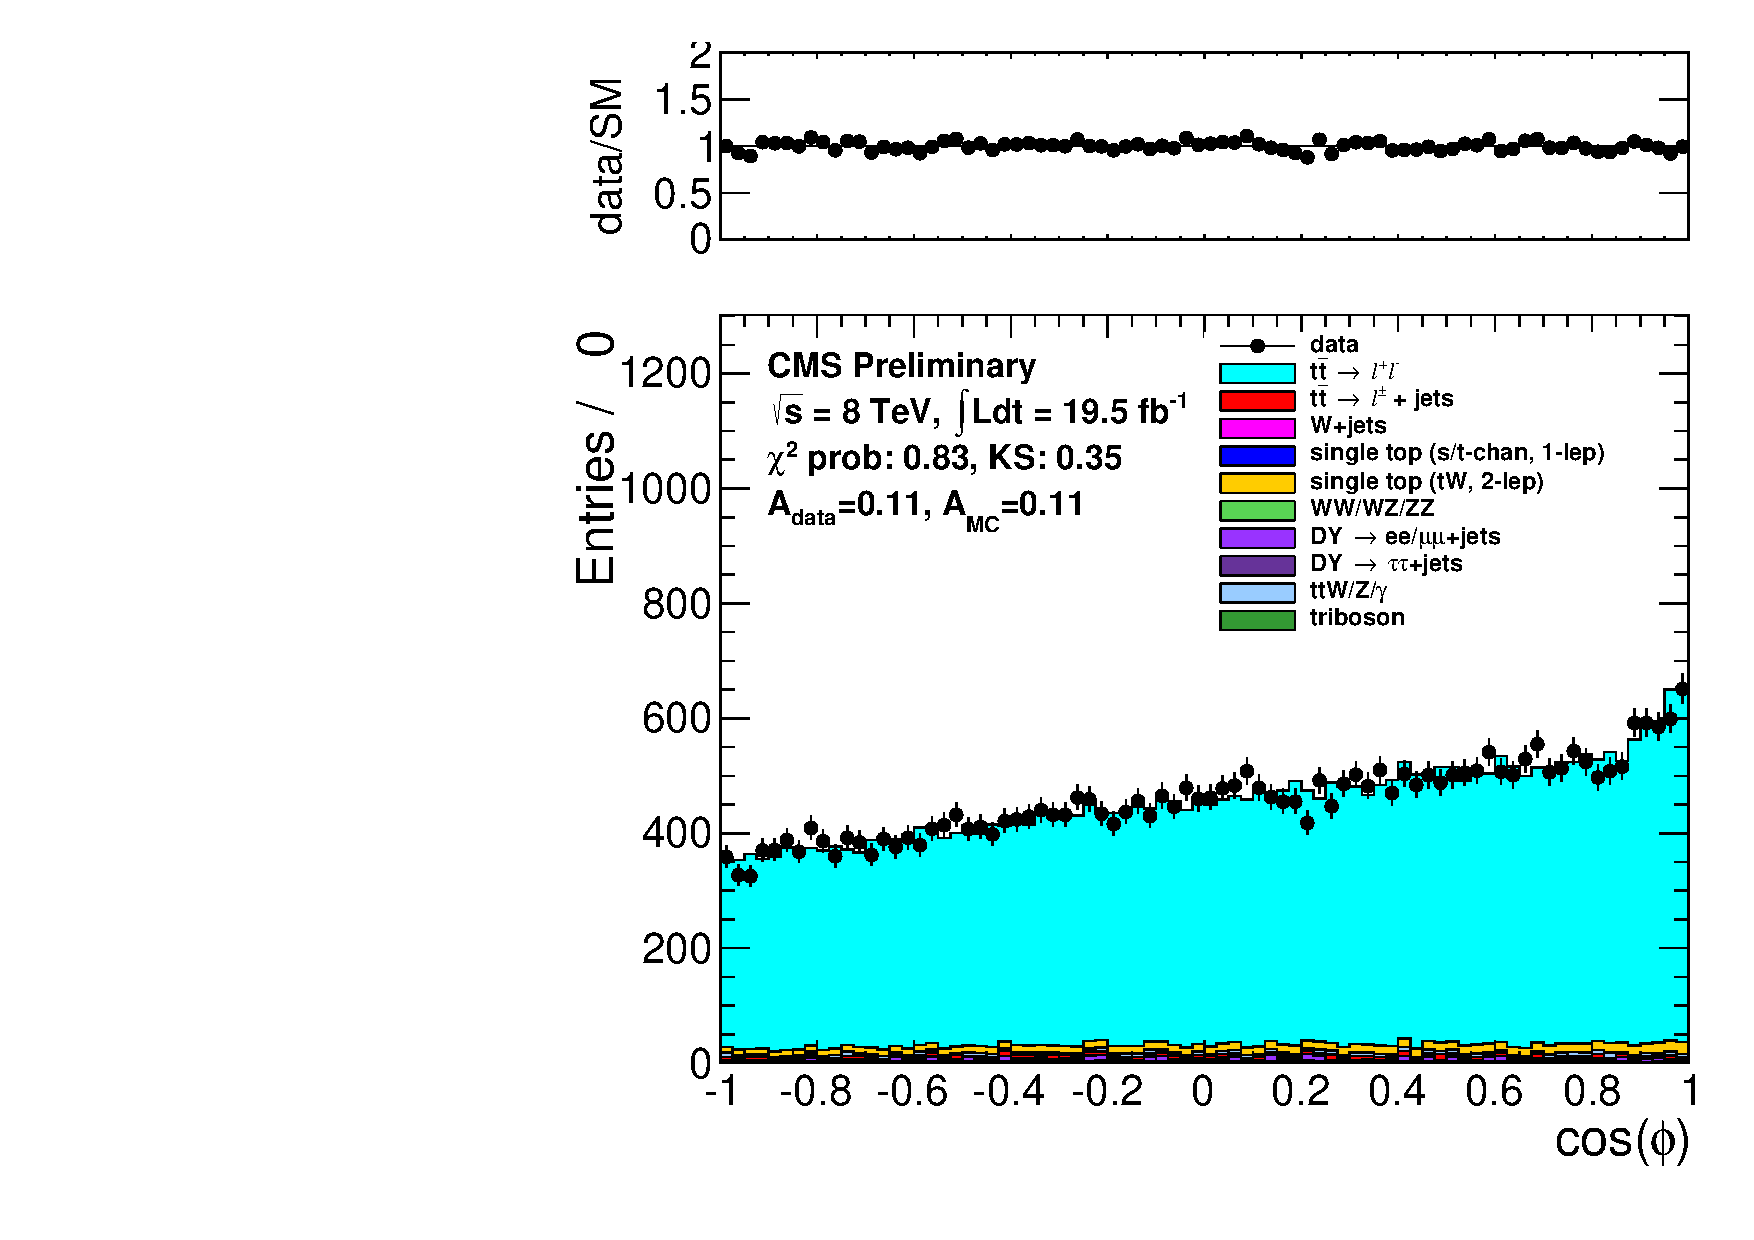
\includegraphics[width=0.325\textwidth]{figures/dataMC_lep_cos_opening_angle_combined.pdf}
  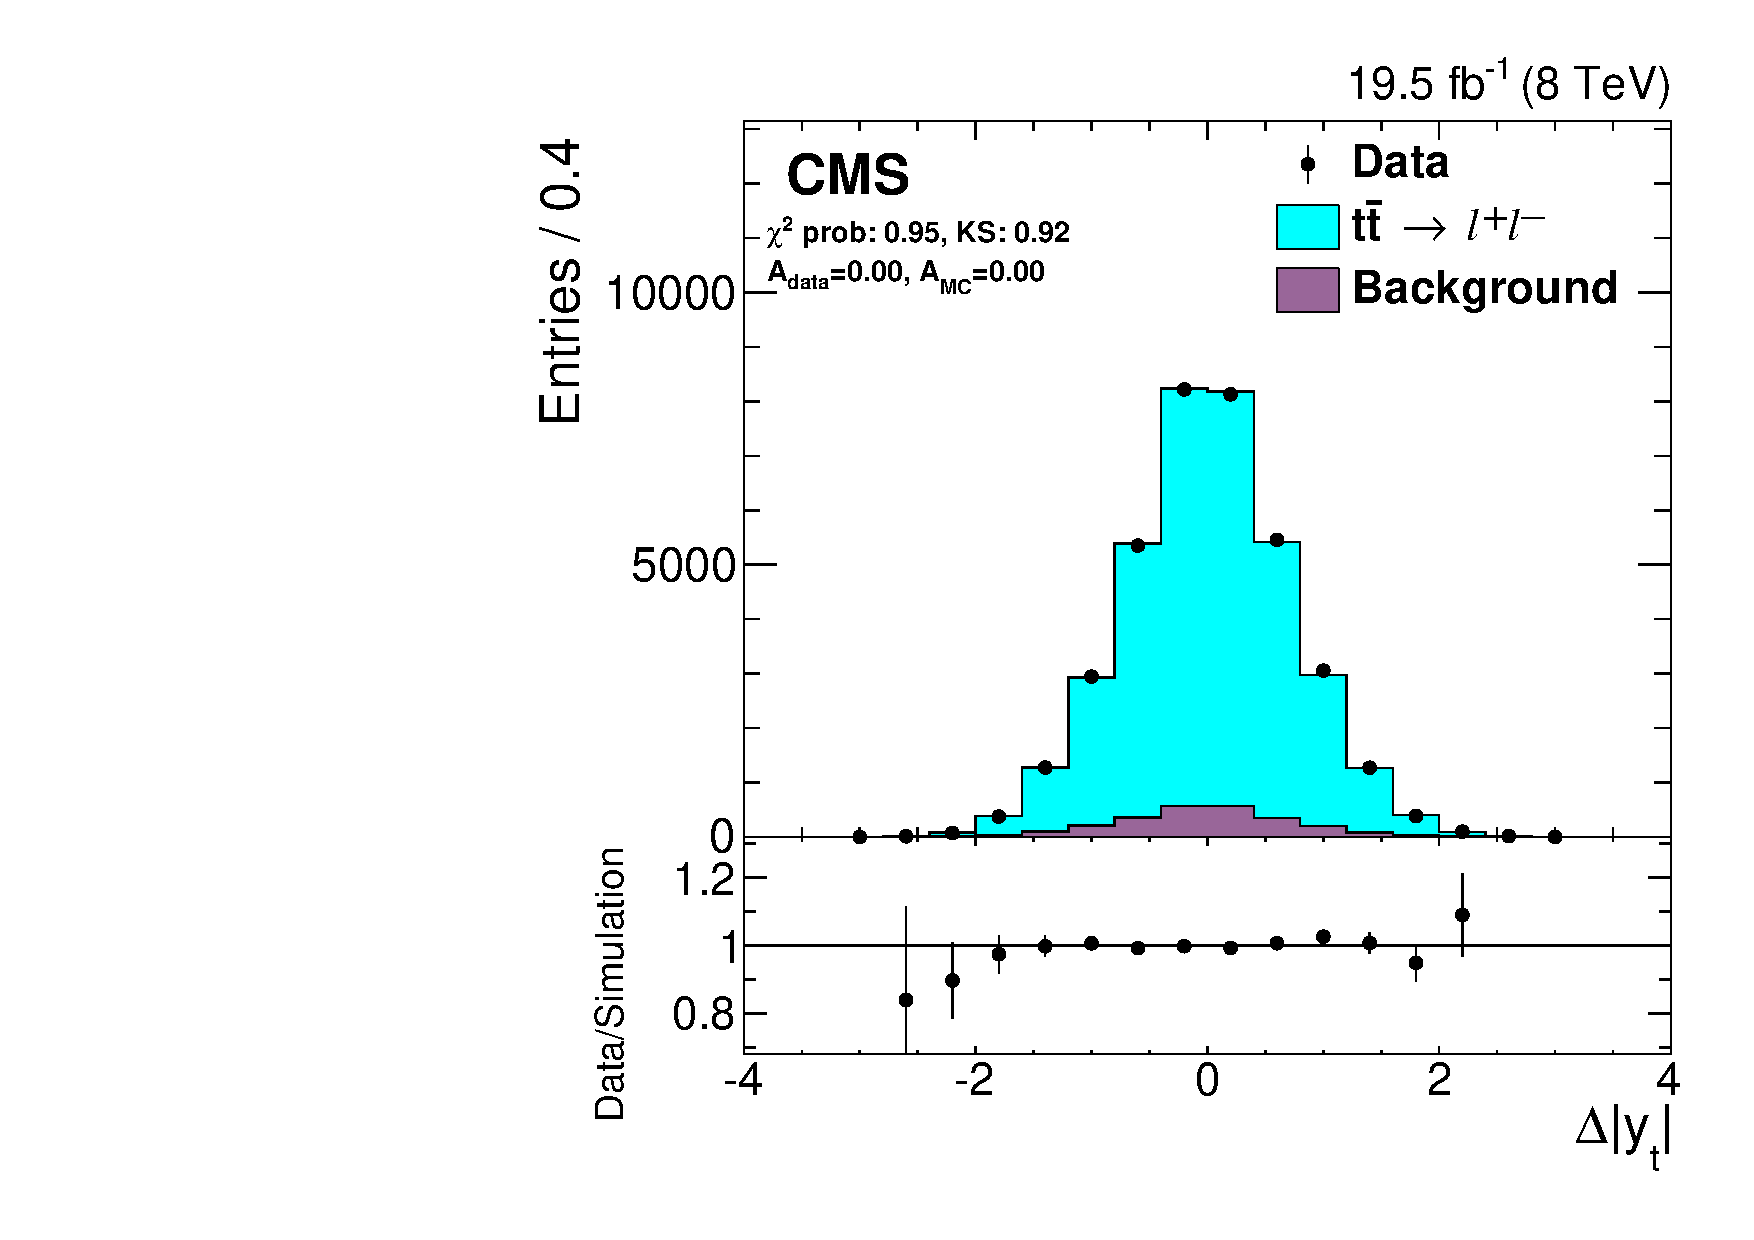
\includegraphics[width=0.325\textwidth]{figures/dataMC_top_rapiditydiff_Marco_combined.pdf}
  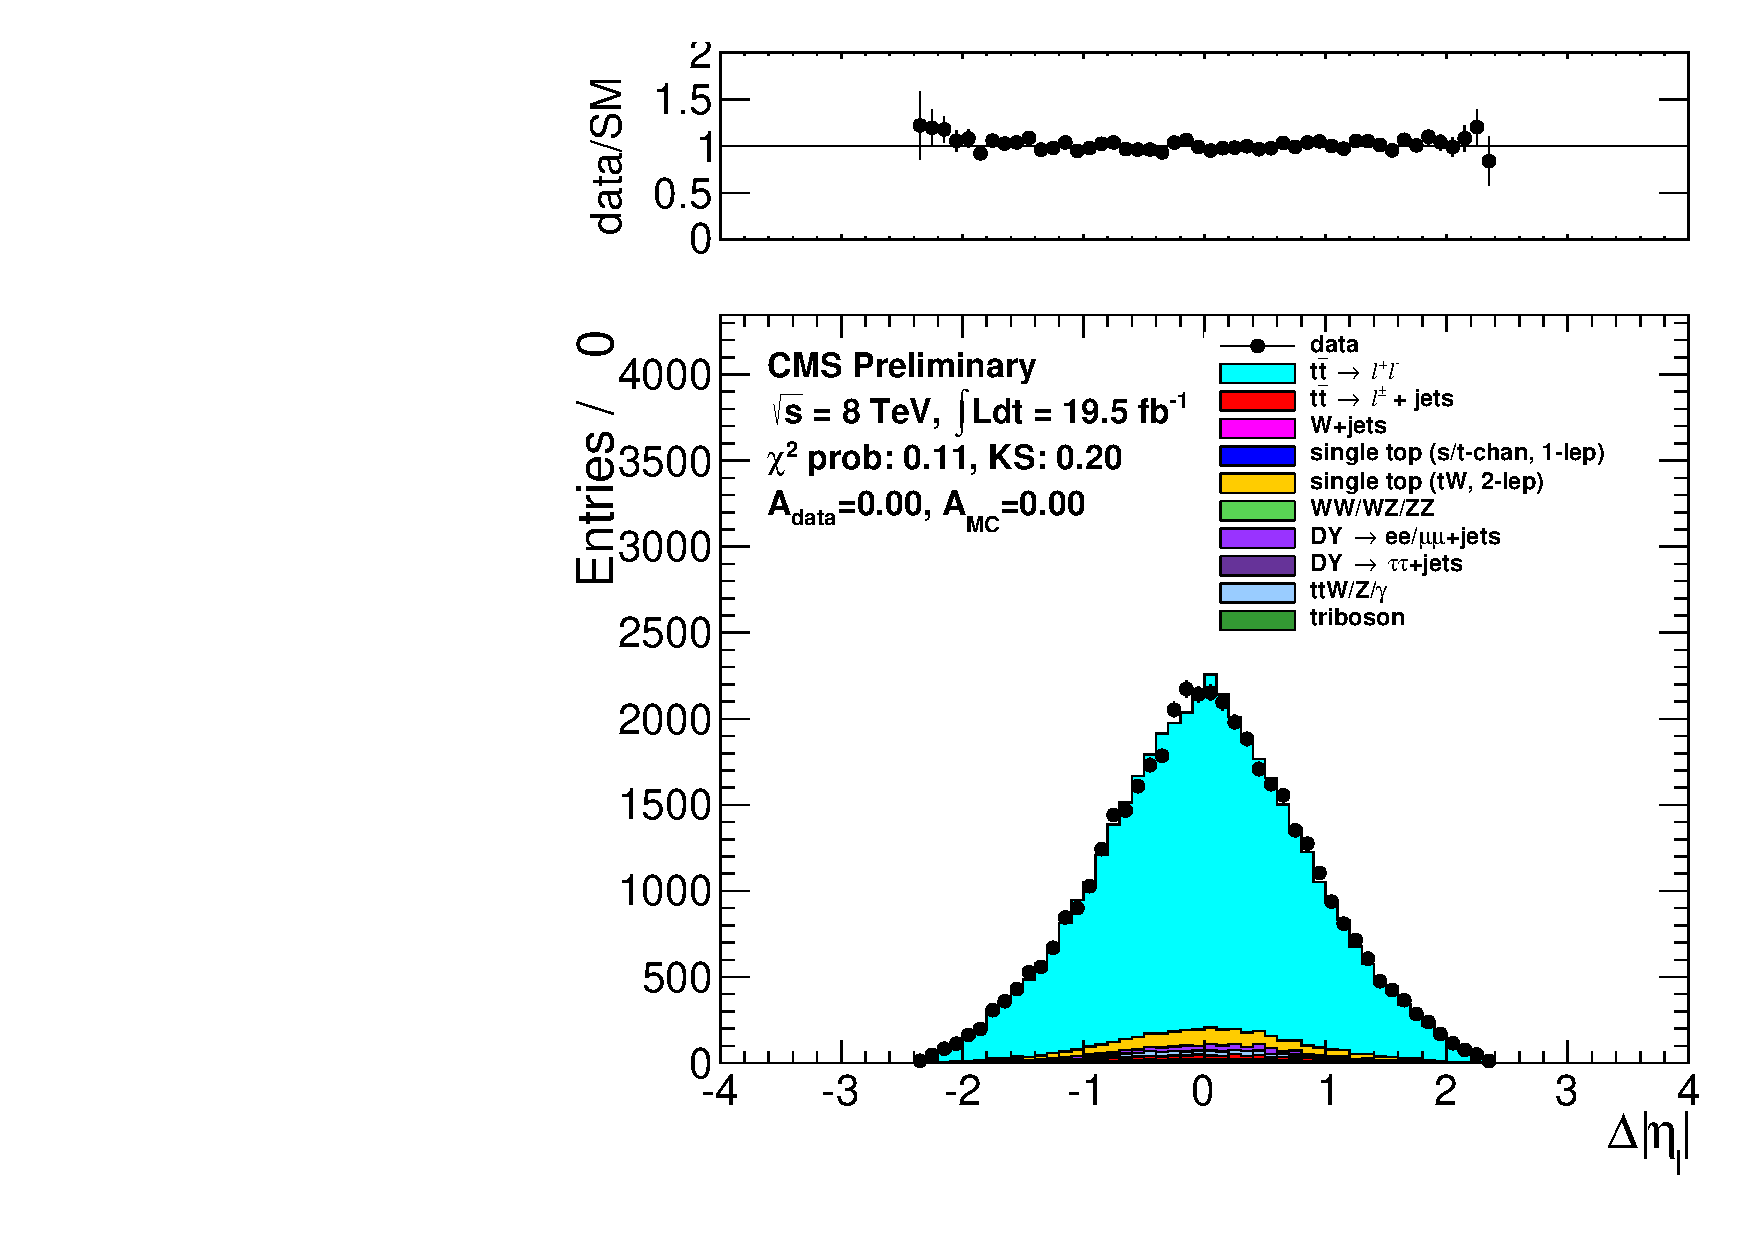
\includegraphics[width=0.325\textwidth]{figures/dataMC_lep_charge_asymmetry_combined.pdf}
  \caption{Comparison of data with Monte Carlo predictions for the
    variables used to compute asymmetries. Helicity angles are
    presented separately for the positively and negatively charged leptons.}
  \label{fig:afb:datamcasymvars}
\end{figure}

\section{Unfolding}
\label{sec:afb:unfolding}

As described in Section \ref{sec:cms}, the CMS detector and its
associated reconstruction software are not perfect, nor are our object
and event selections and reconstruction methods described in Section
\ref{sec:afb:selections}. Because of these imperfections, our measured
asymmetry values may be distorted from the true values.
The unique attributes of other experiments may cause their measured
asymmetry values to differ from those at CMS. And
when theorists make predictions for these asymmetries,
they predict the true values, not the values that would be measured by any
individual experiment. So in order to compare our results with
theoretical predictions, as well as with results measured at other
experiments, it behooves us to extrapolate from our measurements
backward to the true asymmetry values. We do this using a
technique known as \emph{unfolding}.

\subsection{Background}
\label{ssec:afb:unfoldingbkg}

Unfolding is a technique that can be used to reverse blurring or
smearing effects. In other fields it may be known as
\emph{deconvolution} or \emph{unsmearing}. The technique originated in
signal processing and image processing, but its broad utility has seen
it spread to various other scientific and technical
disciplines. Unfolding for particle physics in general is described in detail in
References \cite{unfoldingcowan} and \cite{blobelseminar}. For our
asymmetry measurements, we use the technique as follows:

Each of the physical observables we use to calculate our asymmetries,
such as $\Delta \phi_{\ell\ell}$, may be plotted in a histogram, so that
the contents of each bin correspond to some number of
events. If the bin contents of our measured histogram are expressed as a
vector $\vec{b}$, and the bin contents of the hypothetical ``true''
histogram for that variable are expressed as a vector $\vec{x}$, then we can model the
distorting effects of our detector, reconstruction, etc. using a response
matrix that transforms $\vec{x}$ into $\vec{b}$. We choose to split the
response matrix into two components, $S$ and $A$, giving us the matrix equation:
\begin{equation}
\vec{b} = S A \vec{x}
\label{eq:afb:convolution}
\end{equation}
Here, $A$ is the \emph{acceptance} matrix, a diagonal
matrix that expresses the fraction of true events from each bin that
are actually measured, and not lost to event selection. $S$ is the \emph{smearing}
matrix, which describes the fraction of true events from each bin that
get measured in other bins due to distortion from reconstruction
effects. If we know the values of the matrices $S$ and
$A$, and they are invertible, then we can invert Equation
\ref{eq:afb:convolution} to solve for the true distribution:
\begin{equation}
\vec{x} = A^{-1} S^{-1} \vec{b}
\label{eq:afb:deconvolution}
\end{equation}

Unfolding is an example of an \emph{inverse problem}, because it takes
effects and attempts to extrapolate back to their causes. And like
many other inverse problems, this one is mathematically
\emph{ill-posed}, because a small fluctuation in the measured
distribution $\vec{b}$ can cause a much larger fluctuation in the
unfolded solution $\vec{x}$ \cite{blobelseminar}. To curtail these
fluctuations, we employ a technique called \emph{regularization}.

Regularization is the act of adding additional constraints to the
unfolding process, in the hope of making the unfolded result more
accurate to the true distribution. If we know (or believe) that the
true distribution $\vec{x}$ should have certain properties, we can
constrain the unfolding process so that the output will be more likely
to have those properties too \cite{unfoldingcowan}.

To regularize our unfolded results, we supply the truth-level Monte
Carlo distributions of our variables as \emph{bias distributions},
essentially templates for what the unfolded result should
resemble. In particular, we ask that the unfolded result should attempt
to mimic the curvature (i.e. the second derivative) of the bias
distribution. The strength of the regularization constraint is determined by a
parameter $\tau$. Choosing a small value for $\tau$ will give less
regularization, and lead to more statistical fluctuations in the
output; choosing a large value of $\tau$ will give heavy
regularization, and strongly constrain the output to resemble the bias
distribution. In truth, any amount of regularization must introduce
some degree of bias into our measurements. In Section
\ref{ssec:afb:unfoldingtests}, I describe the tests we perform to
quantify the amount of introduced bias.

\subsection{One-Dimensional Unfolding Procedure}
\label{ssec:afb:unfolding1d}

When choosing how to bin histograms that will be unfolded, one must
strike a balance. If there are too many narrow bins, one risks
causing statistical fluctuations in the output. But
with too few bins, one loses resolution in the measurement. For the asymmetry variables
that require us to reconstruct the $\ttbar$ system, we discovered the
ideal balance was to have six bins in the truth level distribution
$\vec{x}$. However, for the variables that only require lepton
reconstruction, we have more statistics and finer resolution, allowing
us to use 12 bins at truth level. In both cases we use twice as many
bins for the reconstruction-level distribution $\vec{b}$ to avoid a
quirk of the numerical method that would make the problem seem
artificially well-posed \cite{blobelseminar}. We chose to bin our
variables so that the number of events in each bin would be
approximately equal. The specific bins chosen are given in Table
\ref{tab:afb:binning1d}. The reconstruction-level bins are formed by
simply dividing the truth-level bins in half.

% Table of binnings from AN-14-246. Believed unpublished, but could probably be deduced from published plots.
\begin{sidewaystable}
\begin{center}
\caption{Truth-level bins chosen for 1D unfolding of asymmetry variables.}
\label{tab:afb:binning1d}
\begin{tabular}{l |  c  c  c  c  c  c }
\hline
Variable &  B1  &  B2 &  B3 &  B4 &  B5 &  B6\\ \hline
$A_{C}$  &        [-$\infty$,-22/30]  &  [-22/30,-10/30]  &  [-10/30,0]  &  [0, 10/30]  &  [10/30, 22/30]  &  [22/30, $\infty$] \\ \hline
$A_{P}$             &  [-1,-2/3]  &  [-2/3,-1/3]  &  [-1/3,0]  &  [0, 1/3]  &  [1/3, 2/3]  &  [2/3, 1] \\ \hline
$A_{c1c2}$        &  [-1,-2/5]  &  [-2/5,-1/6]  &  [-1/6,0]  &  [0, 1/6]  &  [1/6, 2/5]  &  [2/5, 1] \\ \hline
$A_{\cos\phi}$       &  [-1,-2/3]  &  [-2/3,-1/3]  &  [-1/3,0]  &  [0, 1/3]  &  [1/3, 2/3]  &  [2/3, 1] \\ \hline
\end{tabular}

\bigskip

\begin{tabular}{l |  c  c  c  c  c  c c c c c c c }
\hline
Variable &  B1  &  B2 &  B3 &  B4 &  B5 &  B6 \\ \hline
$A_C^{lep}$  &  [-$\infty$,-34/30]  &  [-34/30,-24/30]  &  [-24/30,-16/30]  &  [-16/30, -10/30]  &  [-10/30, -4/30]  &  [-4/30, 0] \\
\hline
$A_{\Delta\phi}$ &  [0, $5\pi/60$ ]  &  [$5\pi/60$,$10\pi/60$]  &  [$10\pi/60$,$15\pi/60$]  &  [$15\pi/60$, $20\pi/60$]  &  [$20\pi/60$, $25\pi/60$]  &  [$25\pi/60$, $30\pi/60$] \\
\hline \hline
  &  B7 &  B8 &  B9 &  B10 &  B11 &  B12 \\ \hline
$A_C^{lep}$ & [0, 4/30] & [4/30, 10/30] & [10/30, 16/30] & [16/30, 24/30] & [24/30, 34/30] & [34/30, $\infty$] \\ \hline
$A_{\Delta\phi}$ & [$30\pi/60$, $35\pi/60$ ]  &  [$35\pi/60$,$40\pi/60$]  &  [$40\pi/60$,$45\pi/60$]  &  [$45\pi/60$, $50\pi/60$]  &  [$50\pi/60$, $55\pi/60$]  &  [$55\pi/60$, $\pi$] \\ \hline
\end{tabular}
\end{center}
\end{sidewaystable}

For each asymmetry variable, we calculated the fraction of true
Monte Carlo events in each bin that passed our selections. These
values then became the diagonal entries of the acceptance matrix,
$A$. Because our event selections are slightly different for
same-flavor and opposite-flavor dileptons, we calculated and applied
separate acceptance matrices for each case. In Figure \ref{fig:afb:acceptance}, we
show the acceptance matrices for each asymmetry, after combining
the two dilepton flavors in appropriate proportion.

% Acceptance matrices taken from AN-14-246. Unpublished in papers or PASes
\begin{figure}[htpb]
\centering
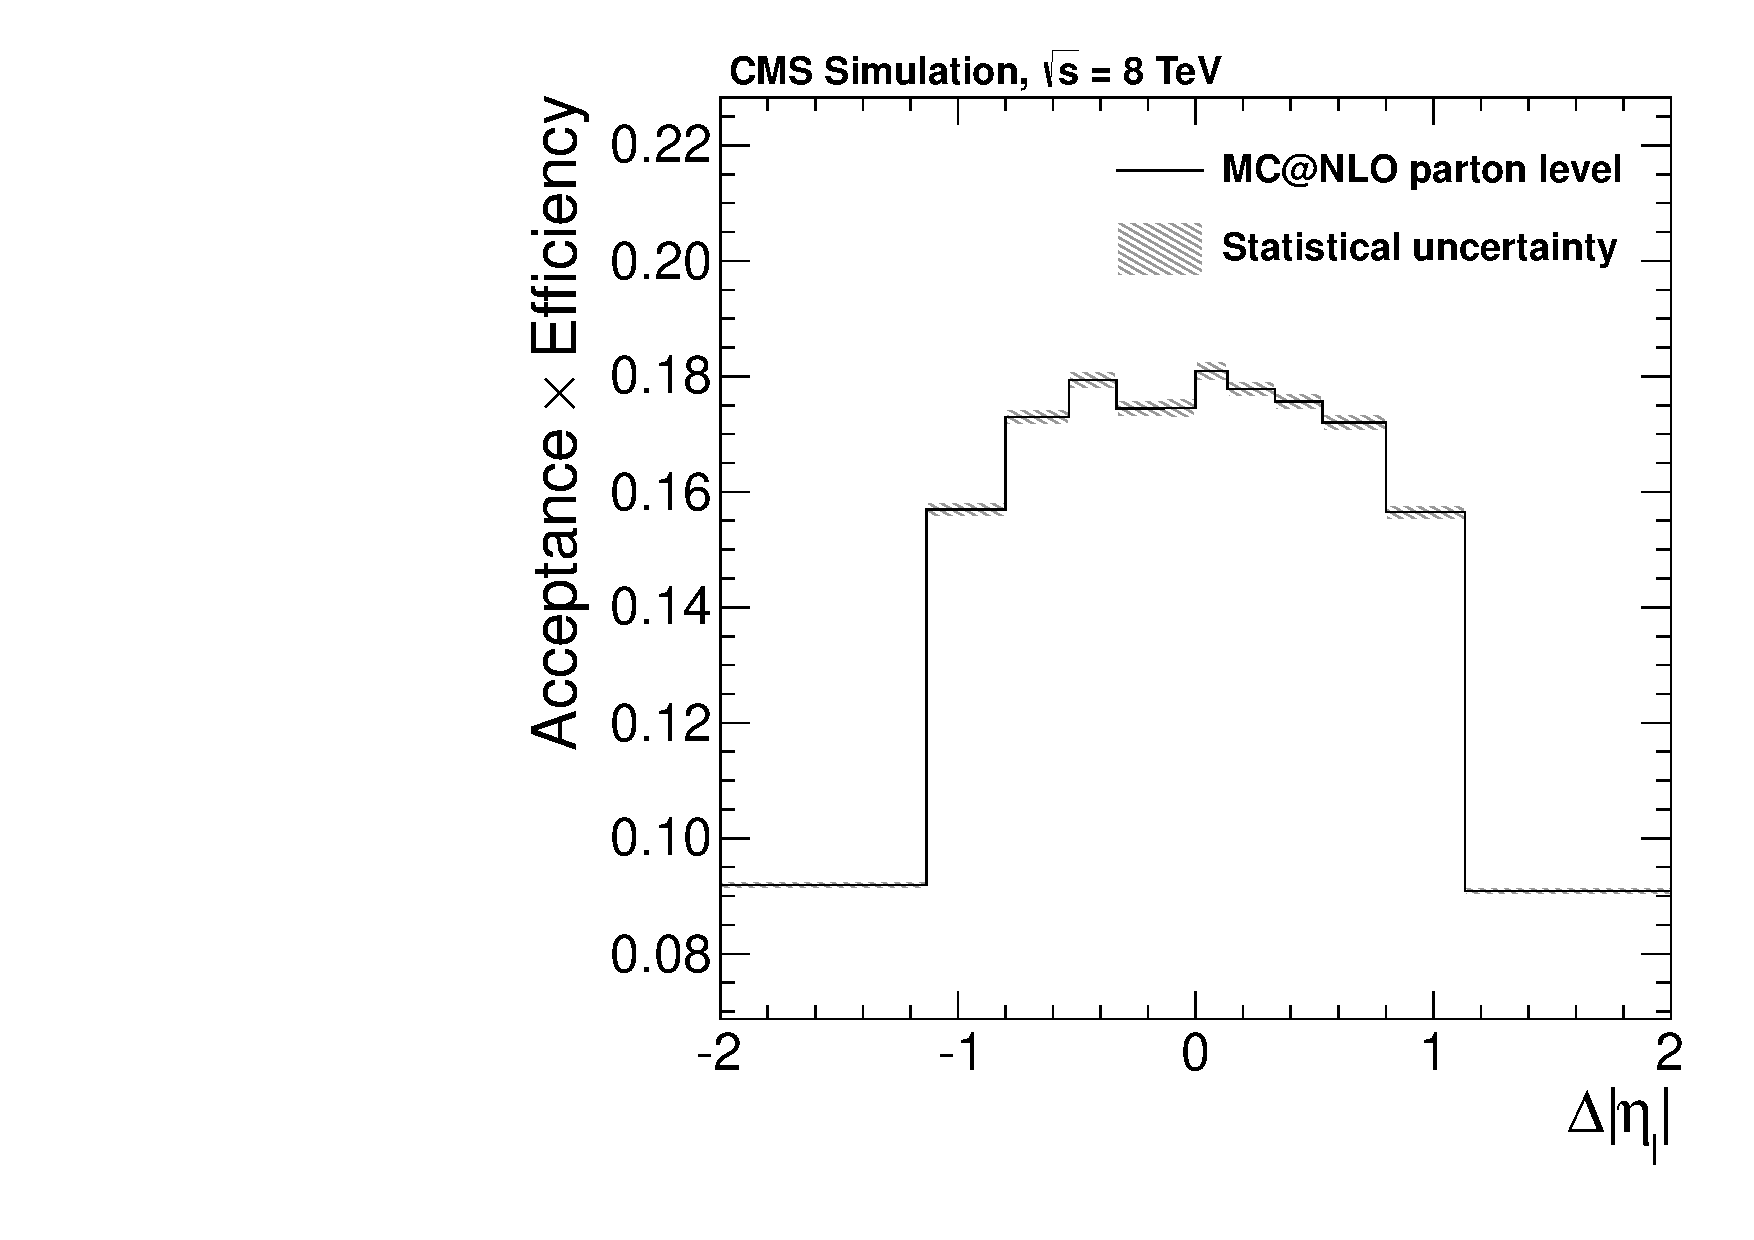
\includegraphics[width=0.325\linewidth]{figures/accept_lepChargeAsym_all.pdf}
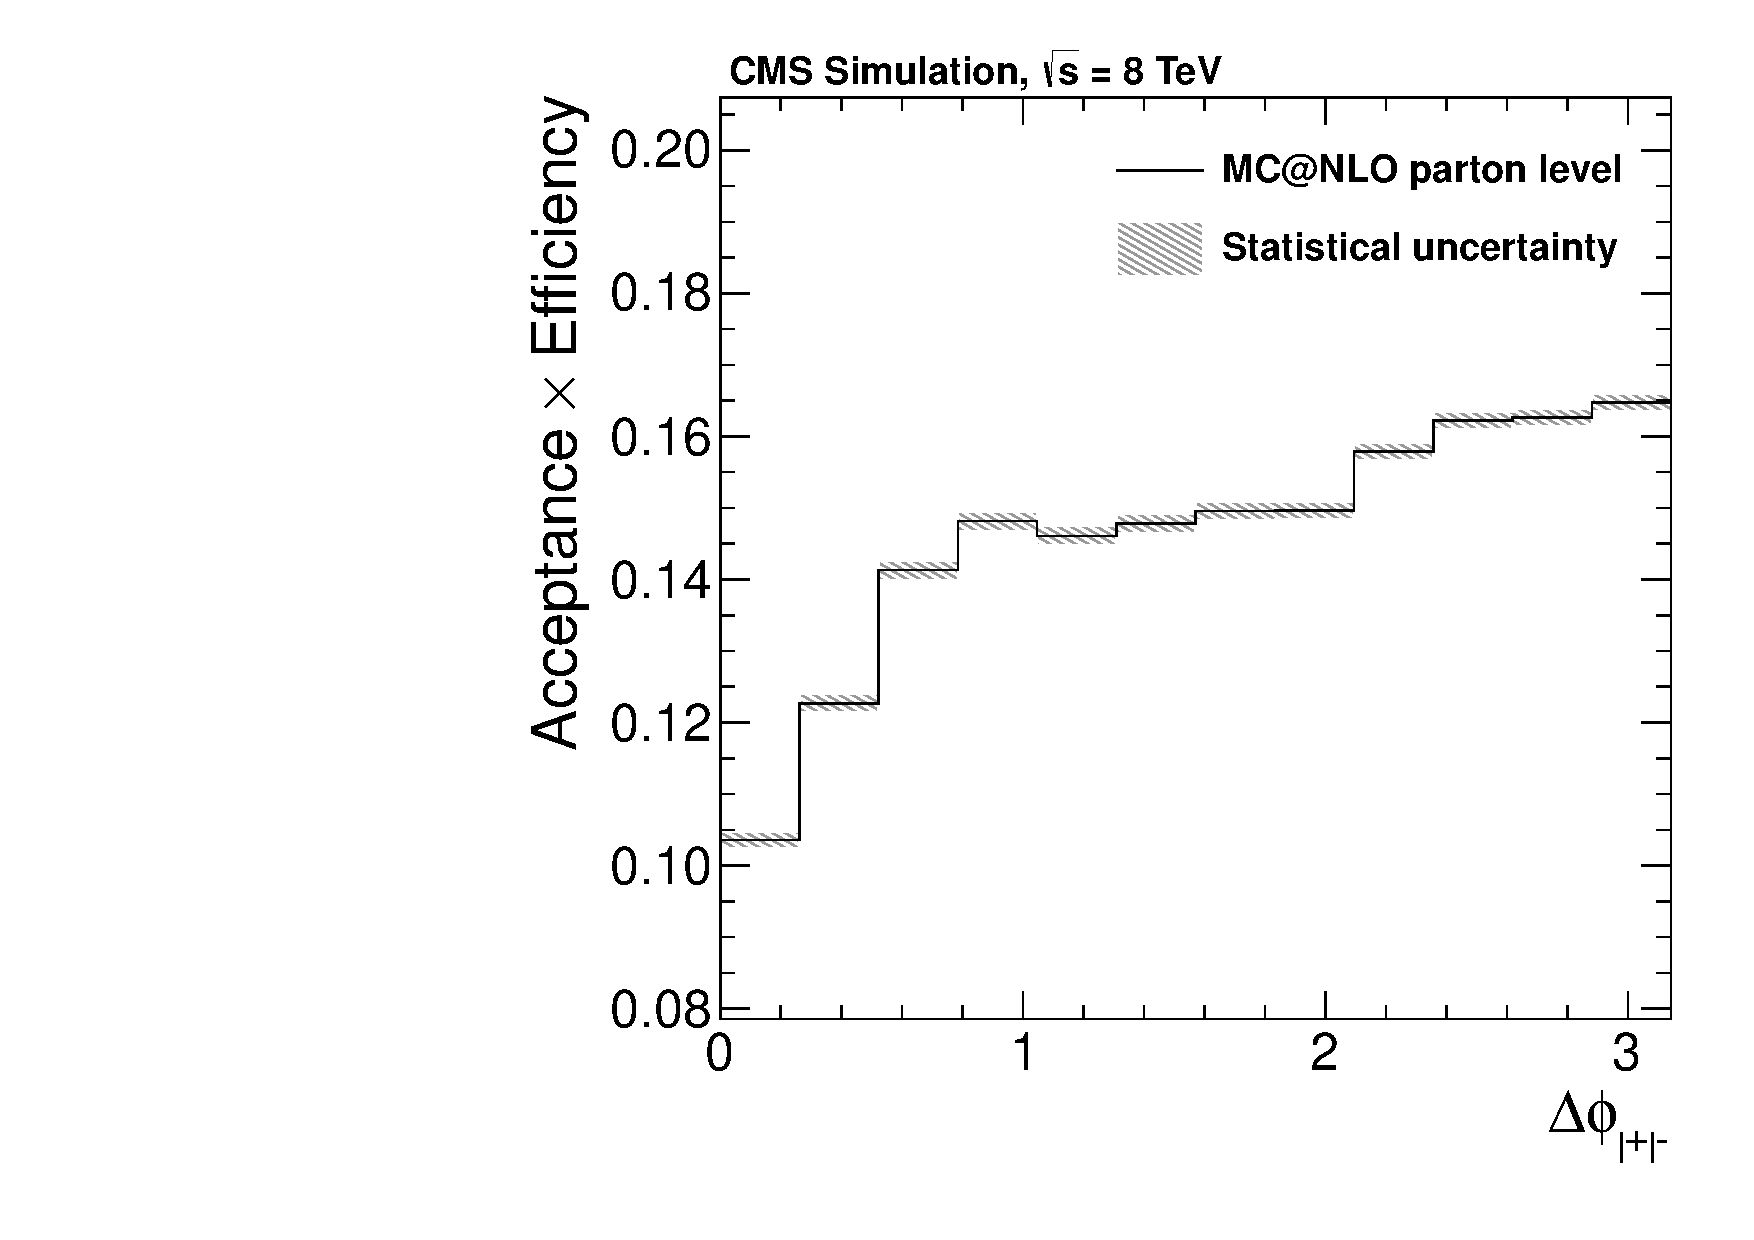
\includegraphics[width=0.325\linewidth]{figures/accept_lepAzimAsym2_all.pdf}
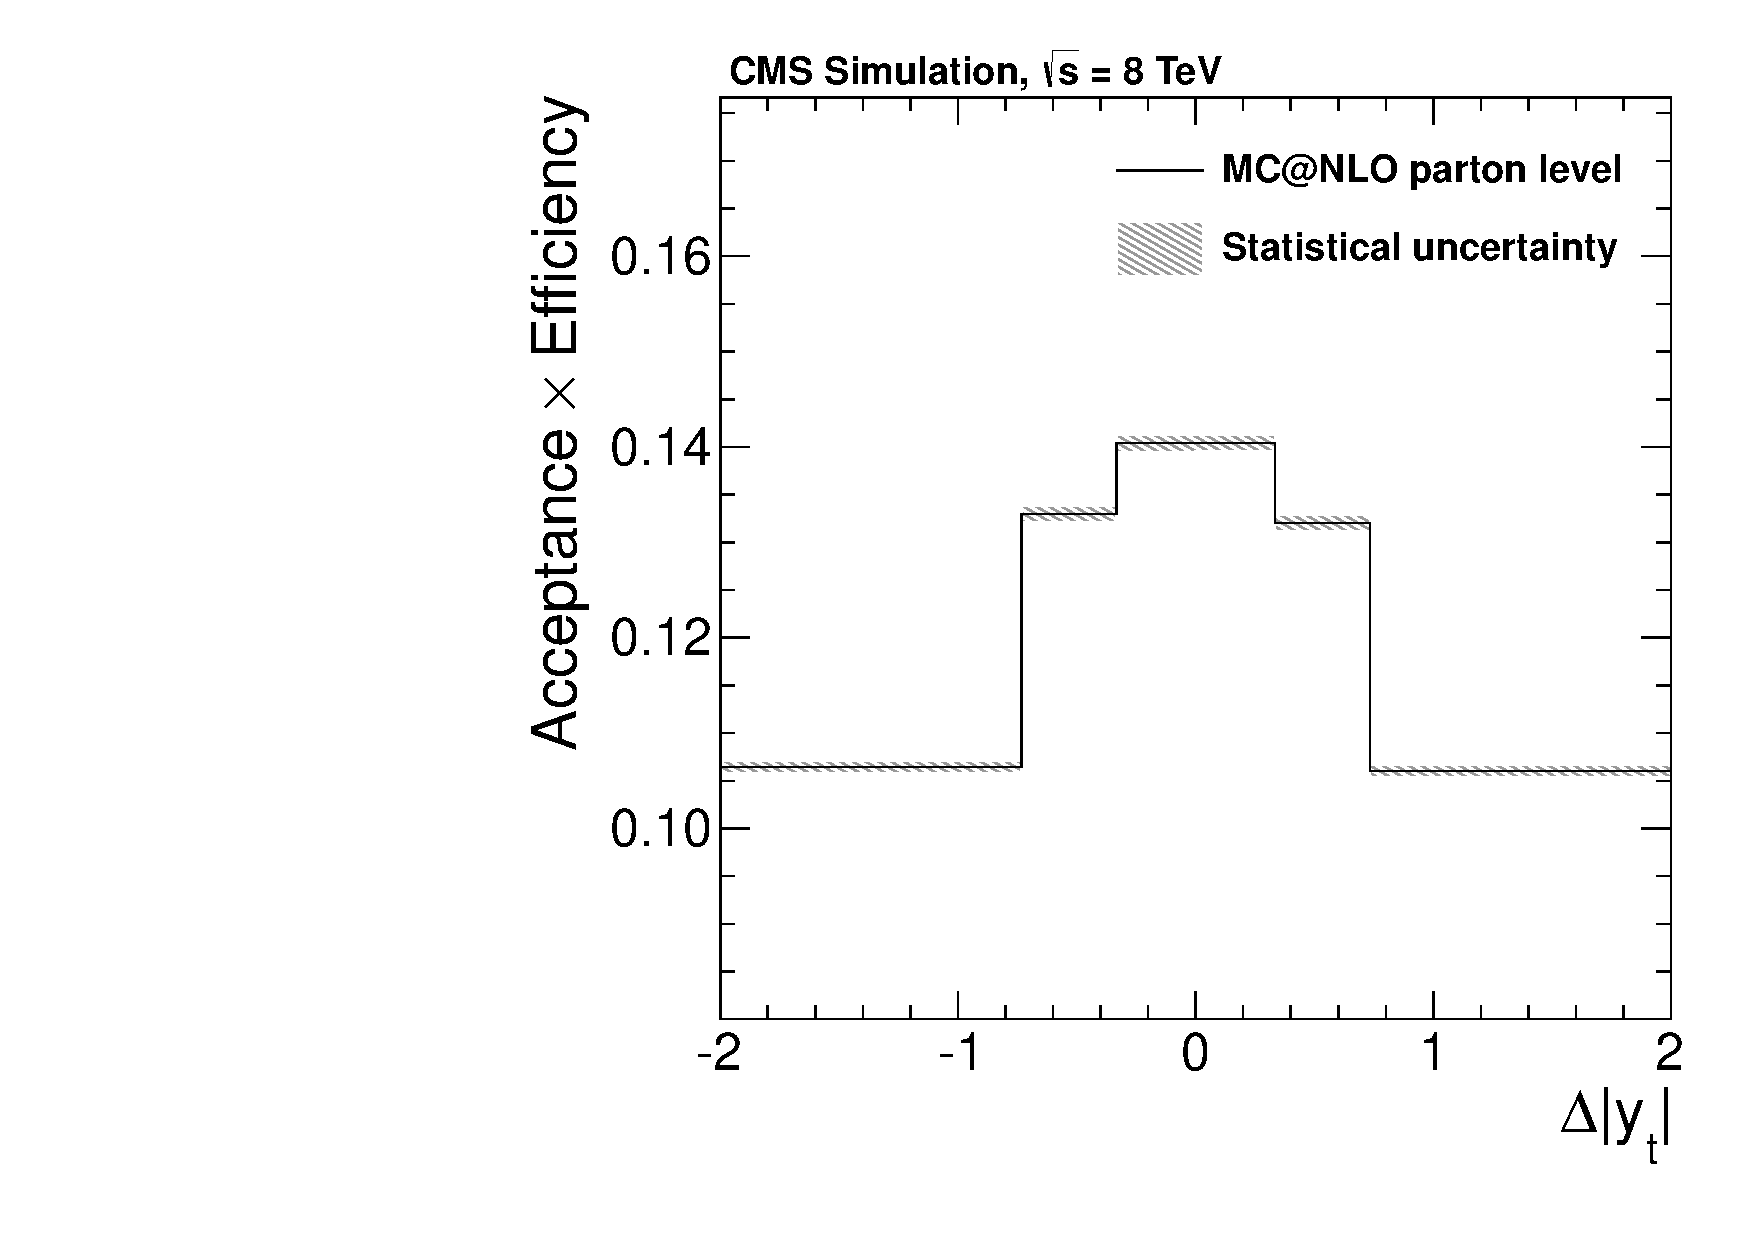
\includegraphics[width=0.325\linewidth]{figures/accept_rapiditydiffMarco_all.pdf}
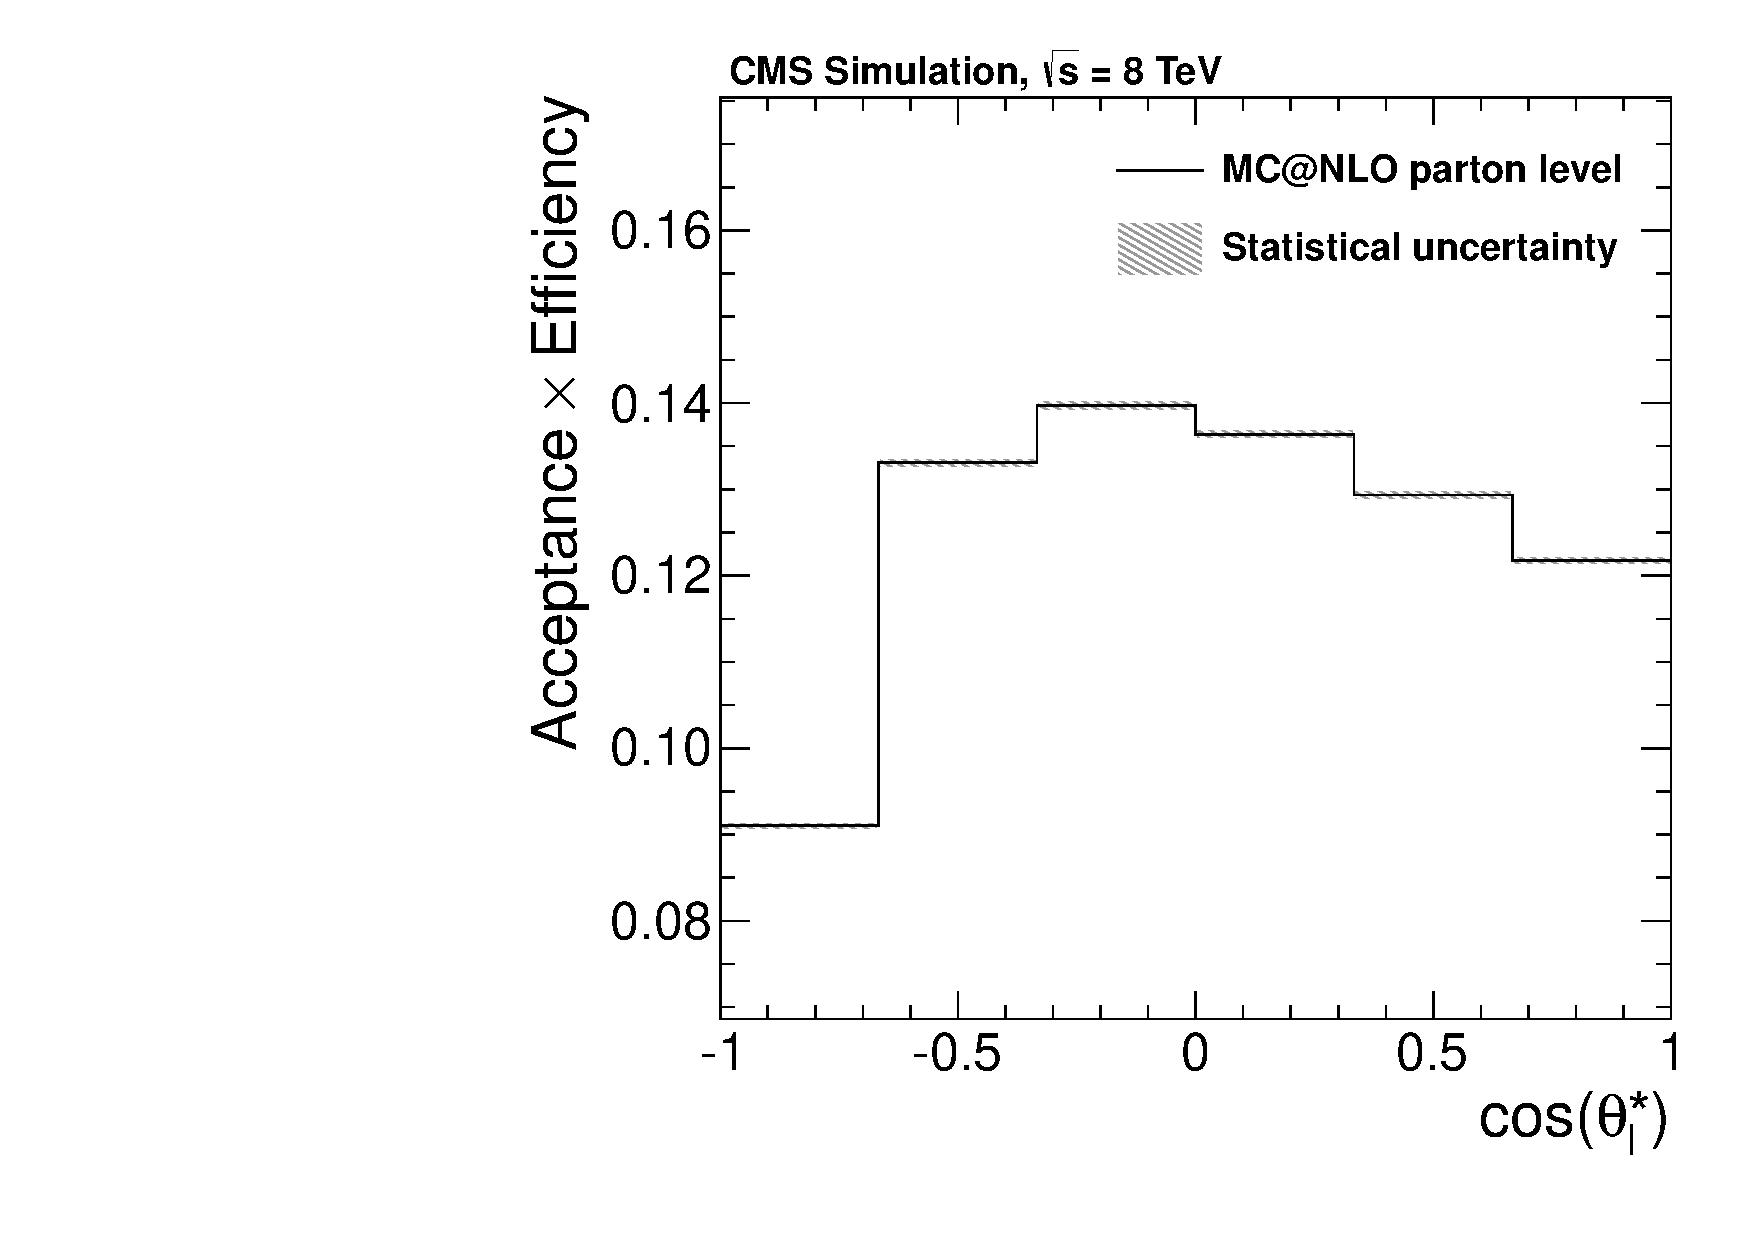
\includegraphics[width=0.325\linewidth]{figures/accept_lepCosTheta_all.pdf}
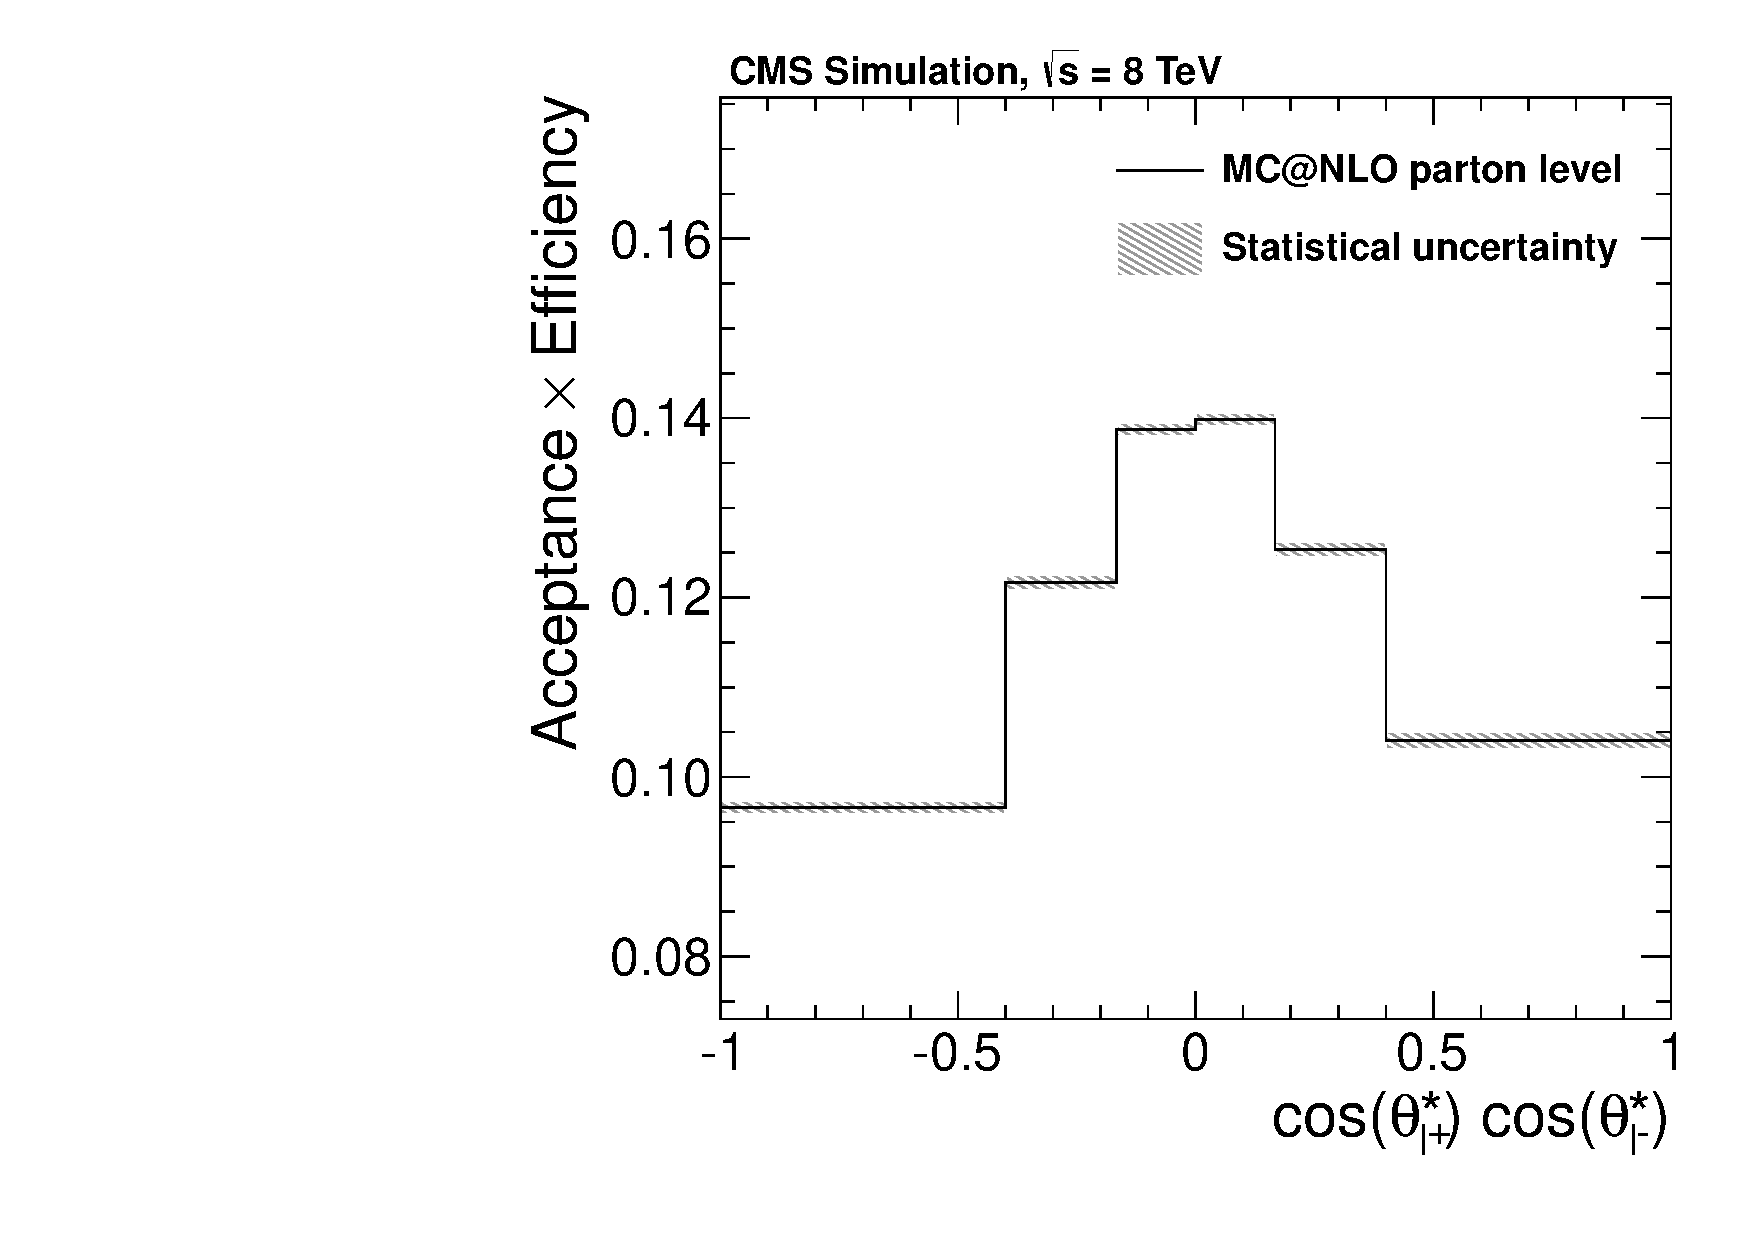
\includegraphics[width=0.325\linewidth]{figures/accept_topSpinCorr_all.pdf}
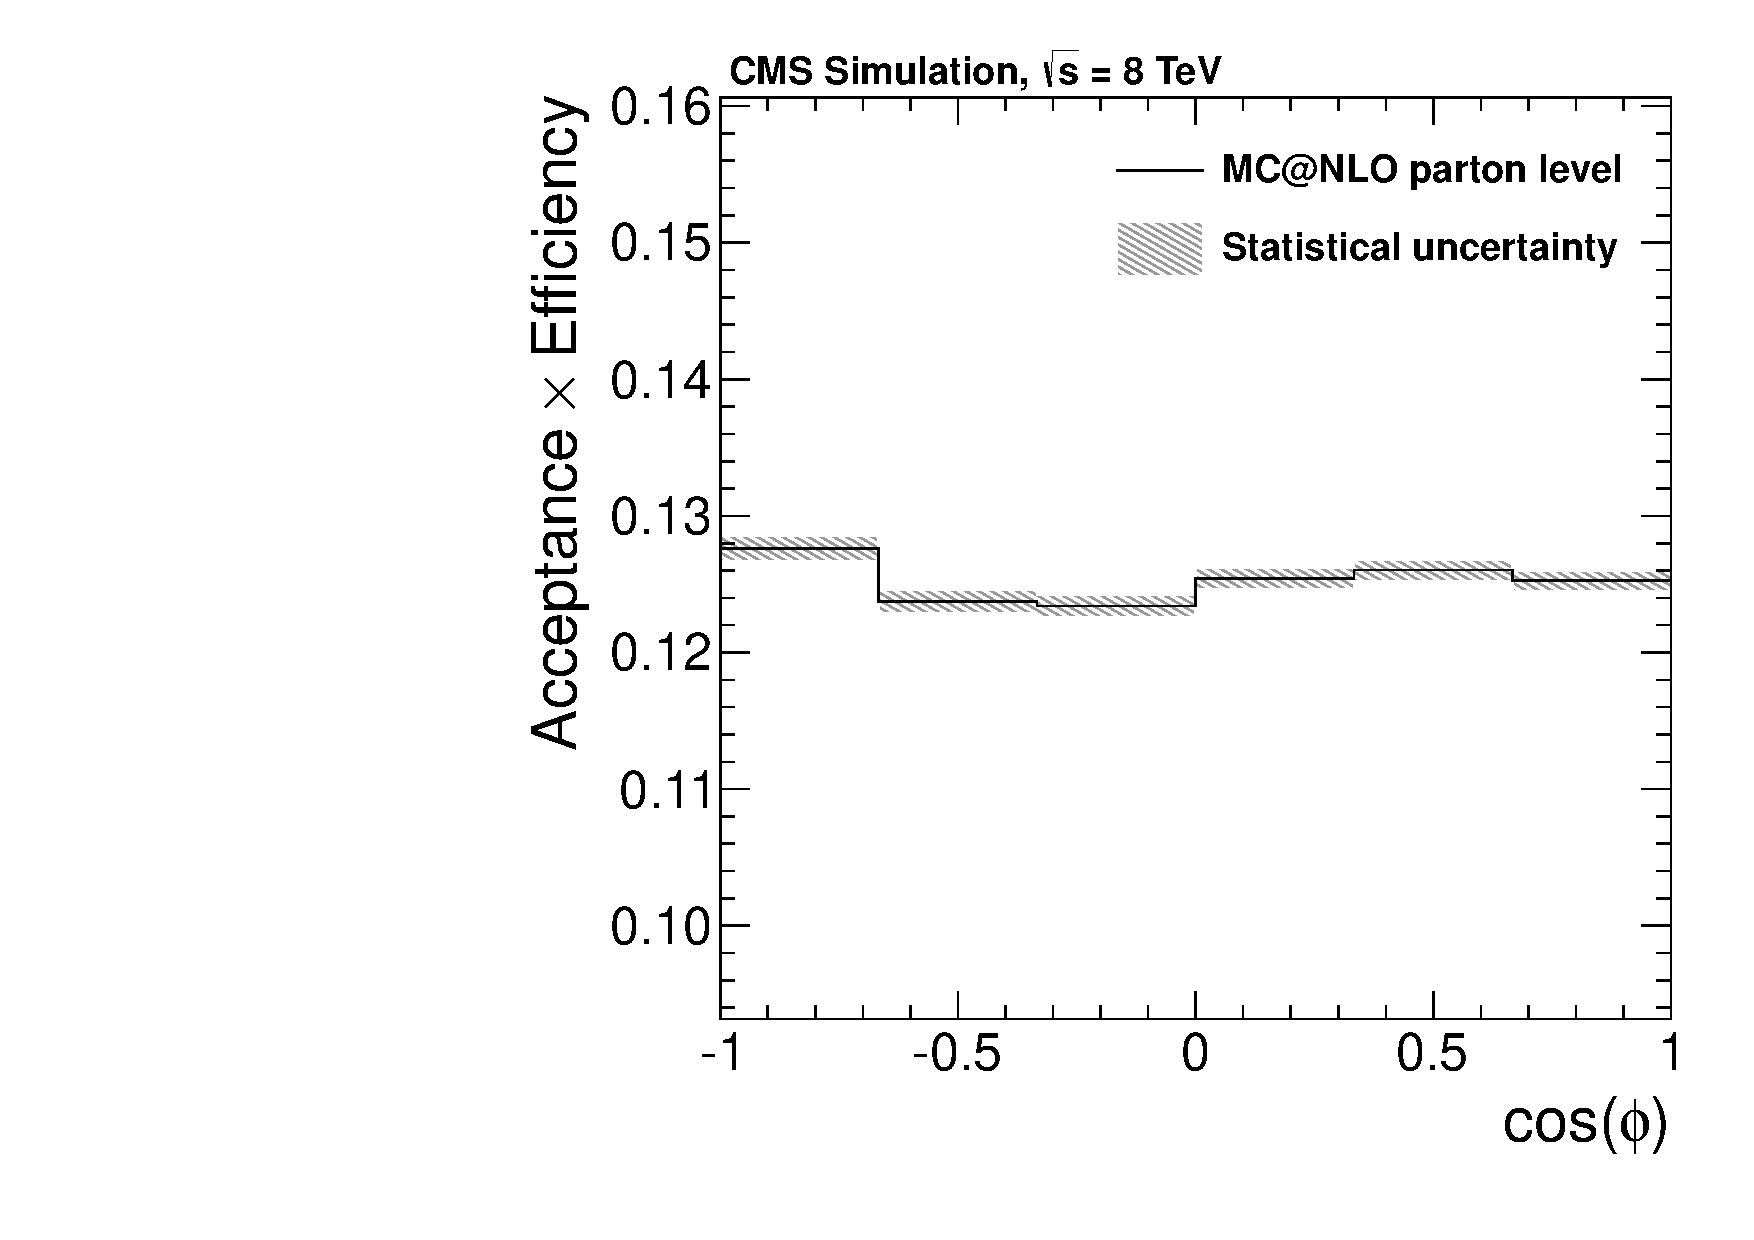
\includegraphics[width=0.325\linewidth]{figures/accept_lepCosOpeningAngle_all.pdf}
\caption{Acceptance matrices for the six asymmetry variables. Since
  all off-diagonal matrix elements are zero, only the diagonal elements are plotted.}
\label{fig:afb:acceptance}
\end{figure}

The smearing matrices $S$ were generated based on Monte Carlo
simulations. Each simulated event was put into a 2D histogram with the
gen-level asymmetry variable on the y-axis and the reco-level
asymmetry variable on the x-axis. The unfolding software then
converted the histogram bins into elements of the smearing
matrix. These histograms are presented in Figure
\ref{fig:afb:smearing}. The histograms that represent the smearing
matrices for the leptonic variables have almost no off-diagonal
components, reflecting the high quality of our lepton
reconstruction. For the variables that require $\ttbar$ system
reconstruction, the smearing is noticeable, and may be due to detector
effects or to the limitations of the $\ttbar$ reconstruction
software. At any rate, these smearing matrices are nearly symmetric
about the diagonal. This fact indicates that reconstruction introduces
little to no bias, and simply dilutes the true asymmetry.

% Smearing matrices taken from AN-14-246. Not published in papers or PASes.
\begin{figure}[htpb]
\centering
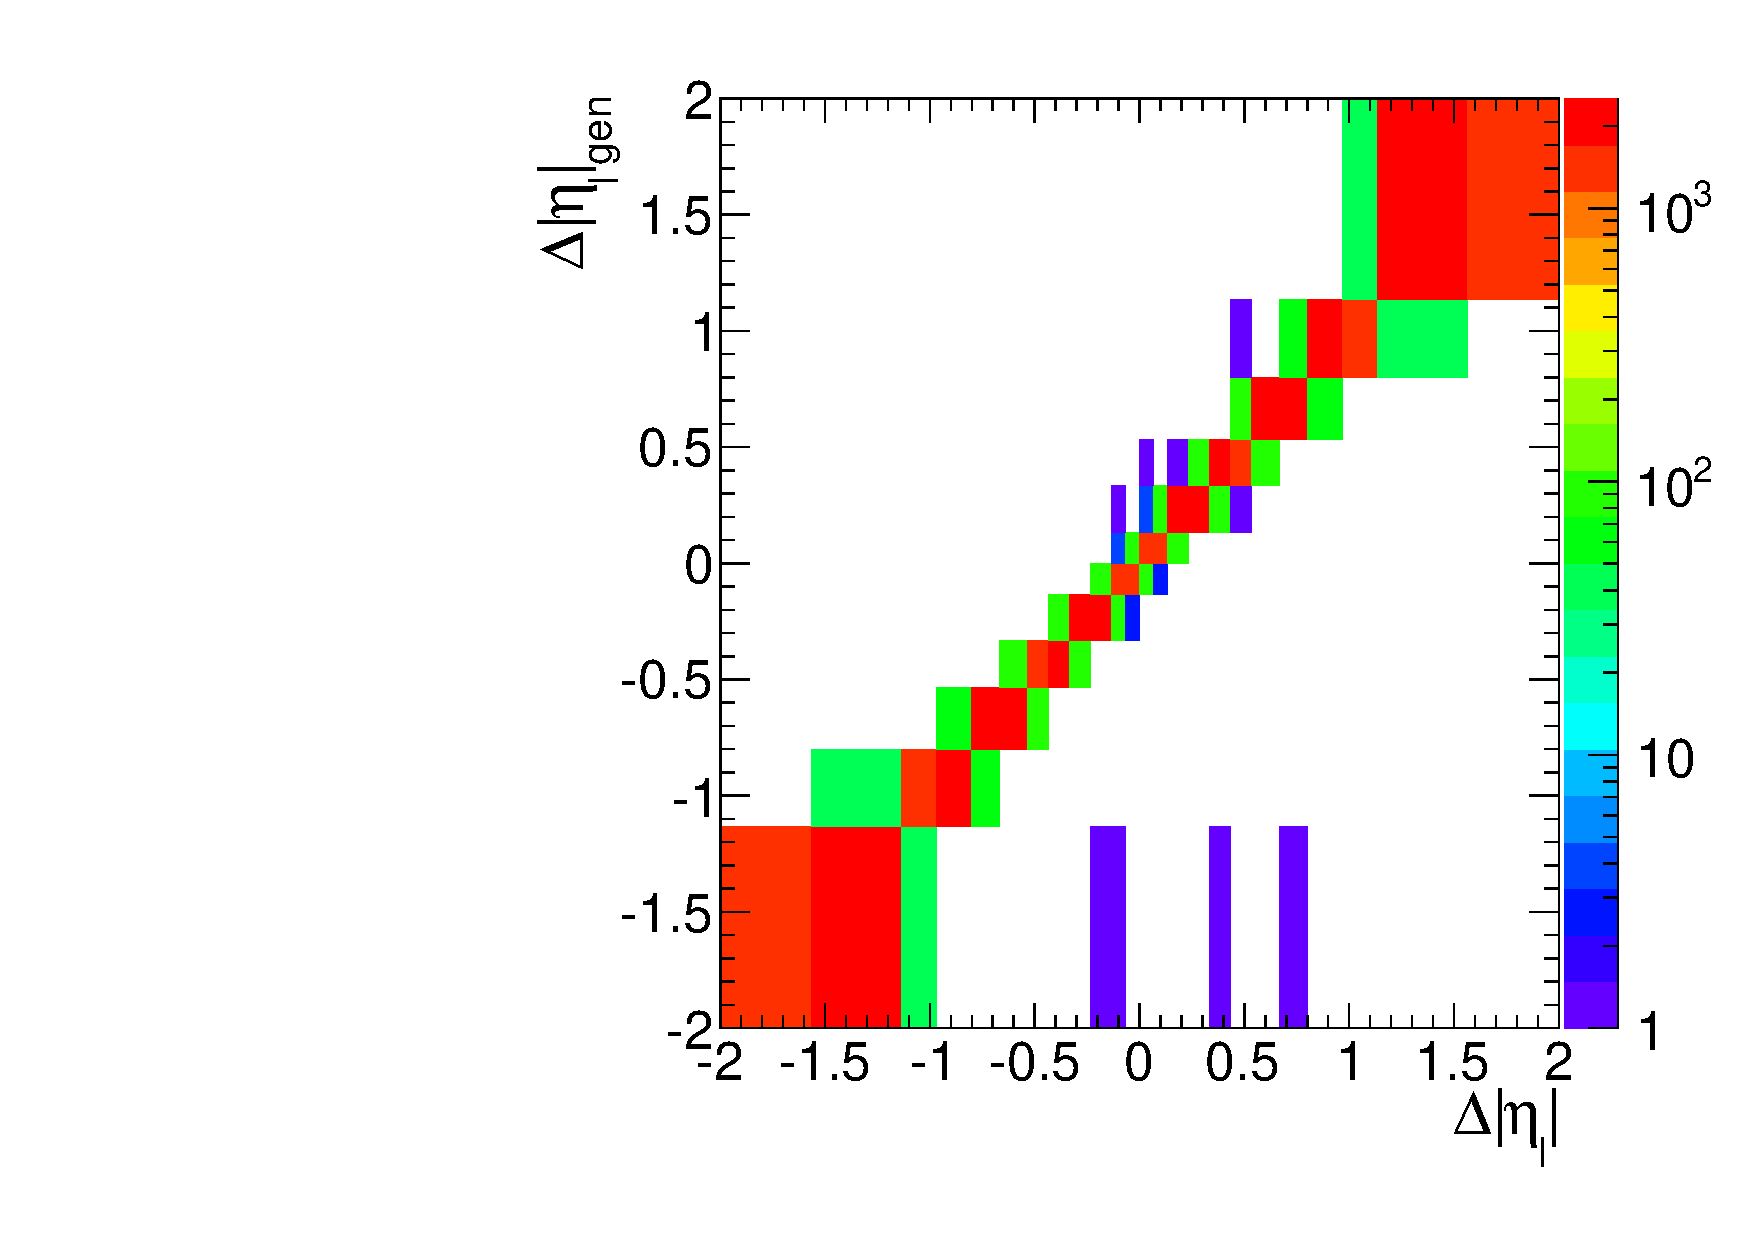
\includegraphics[width=0.325\linewidth]{figures/smearing_lepChargeAsym_all.pdf}
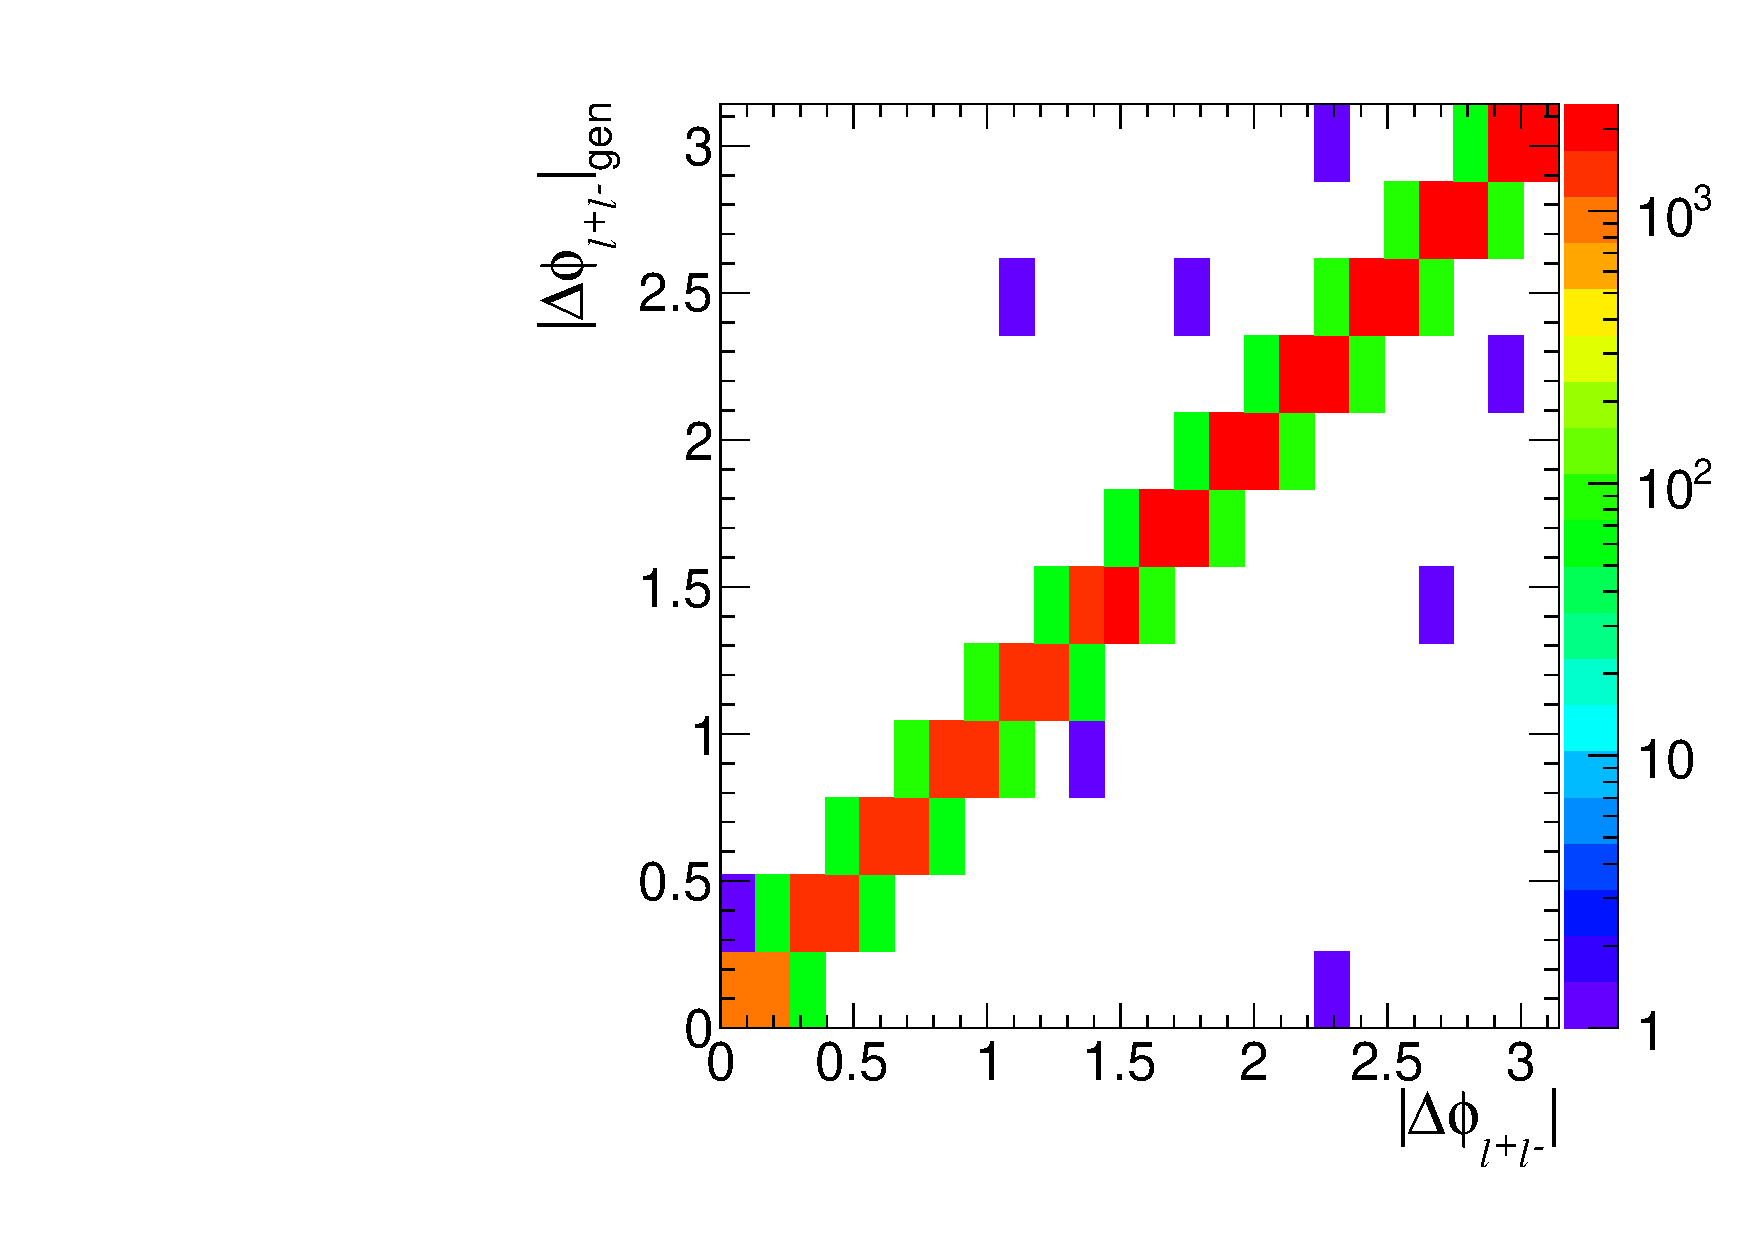
\includegraphics[width=0.325\linewidth]{figures/smearing_lepAzimAsym2_all.pdf}
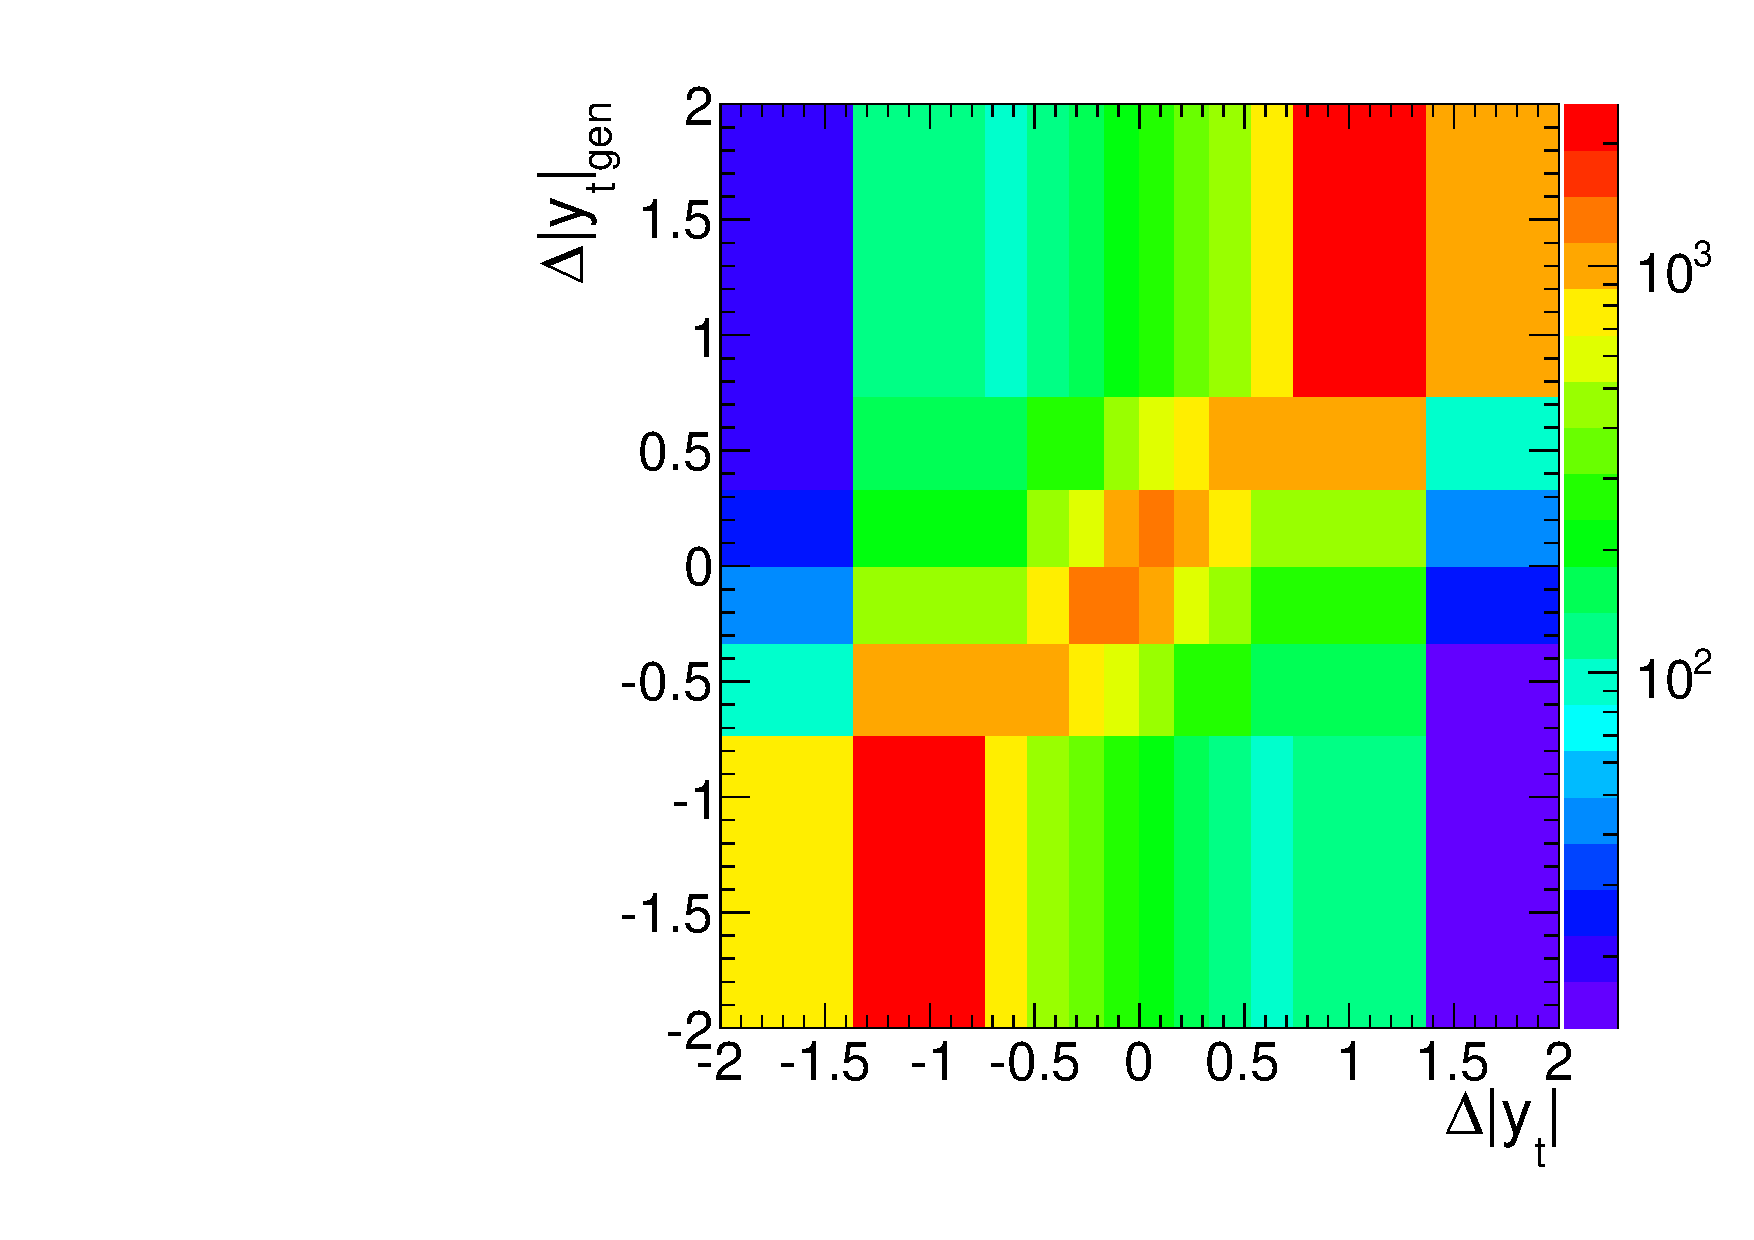
\includegraphics[width=0.325\linewidth]{figures/smearing_rapiditydiffMarco_all.pdf}
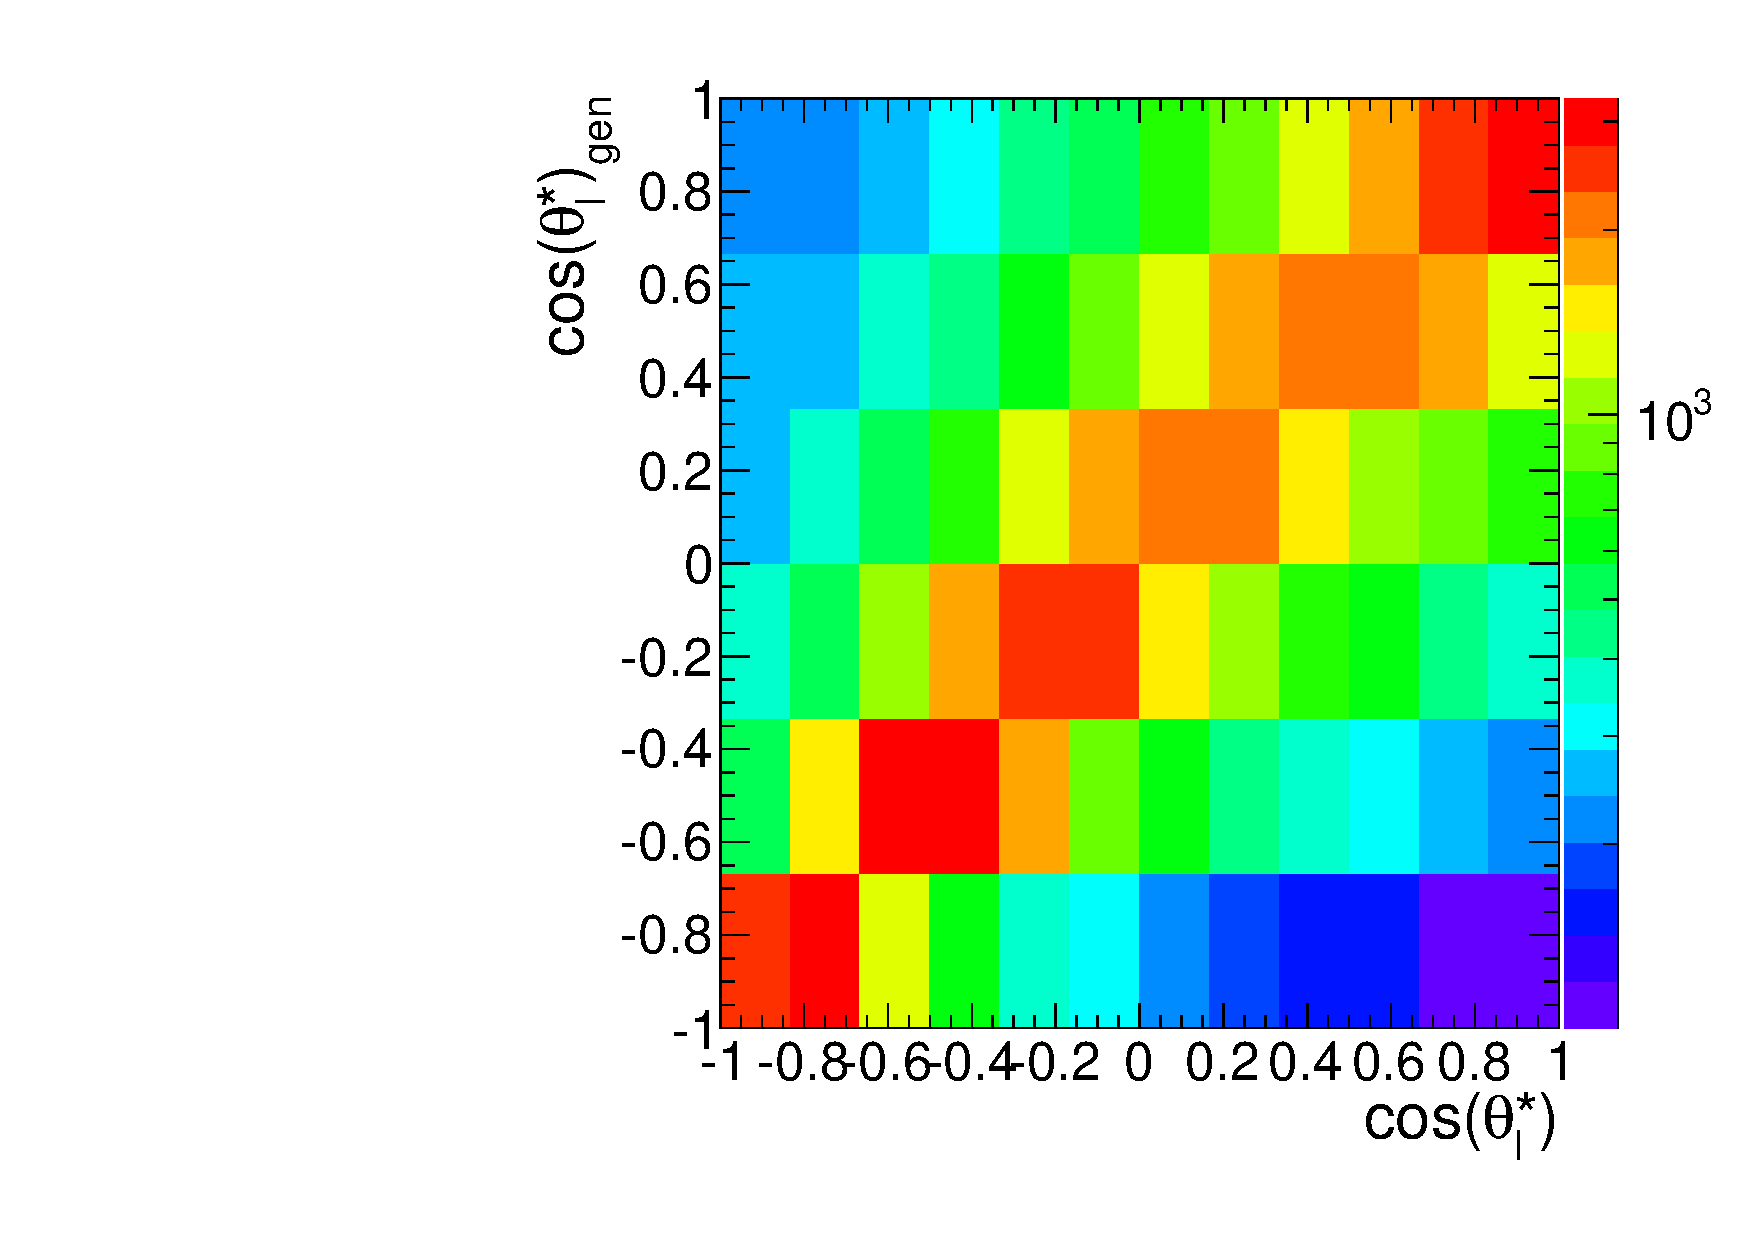
\includegraphics[width=0.325\linewidth]{figures/smearing_lepCosTheta_all.pdf}
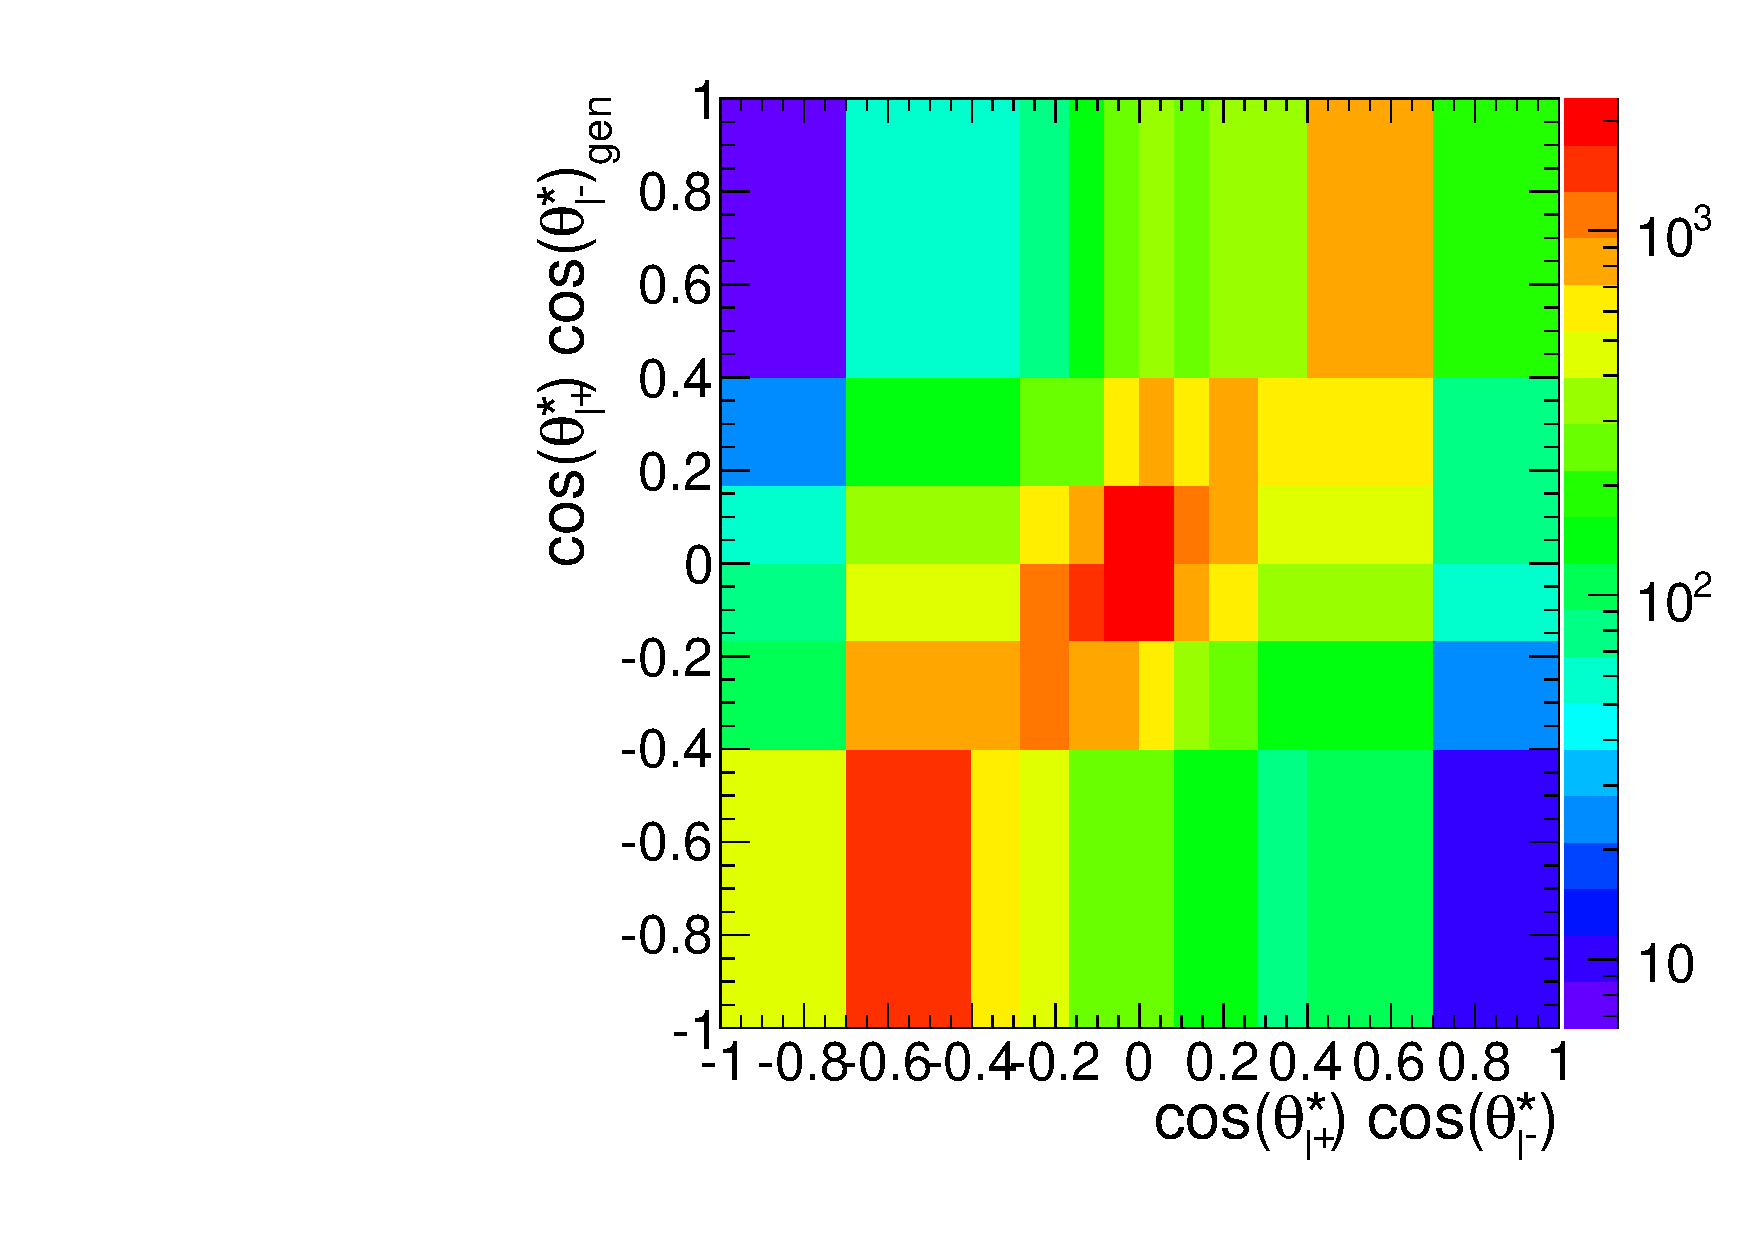
\includegraphics[width=0.325\linewidth]{figures/smearing_topSpinCorr_all.pdf}
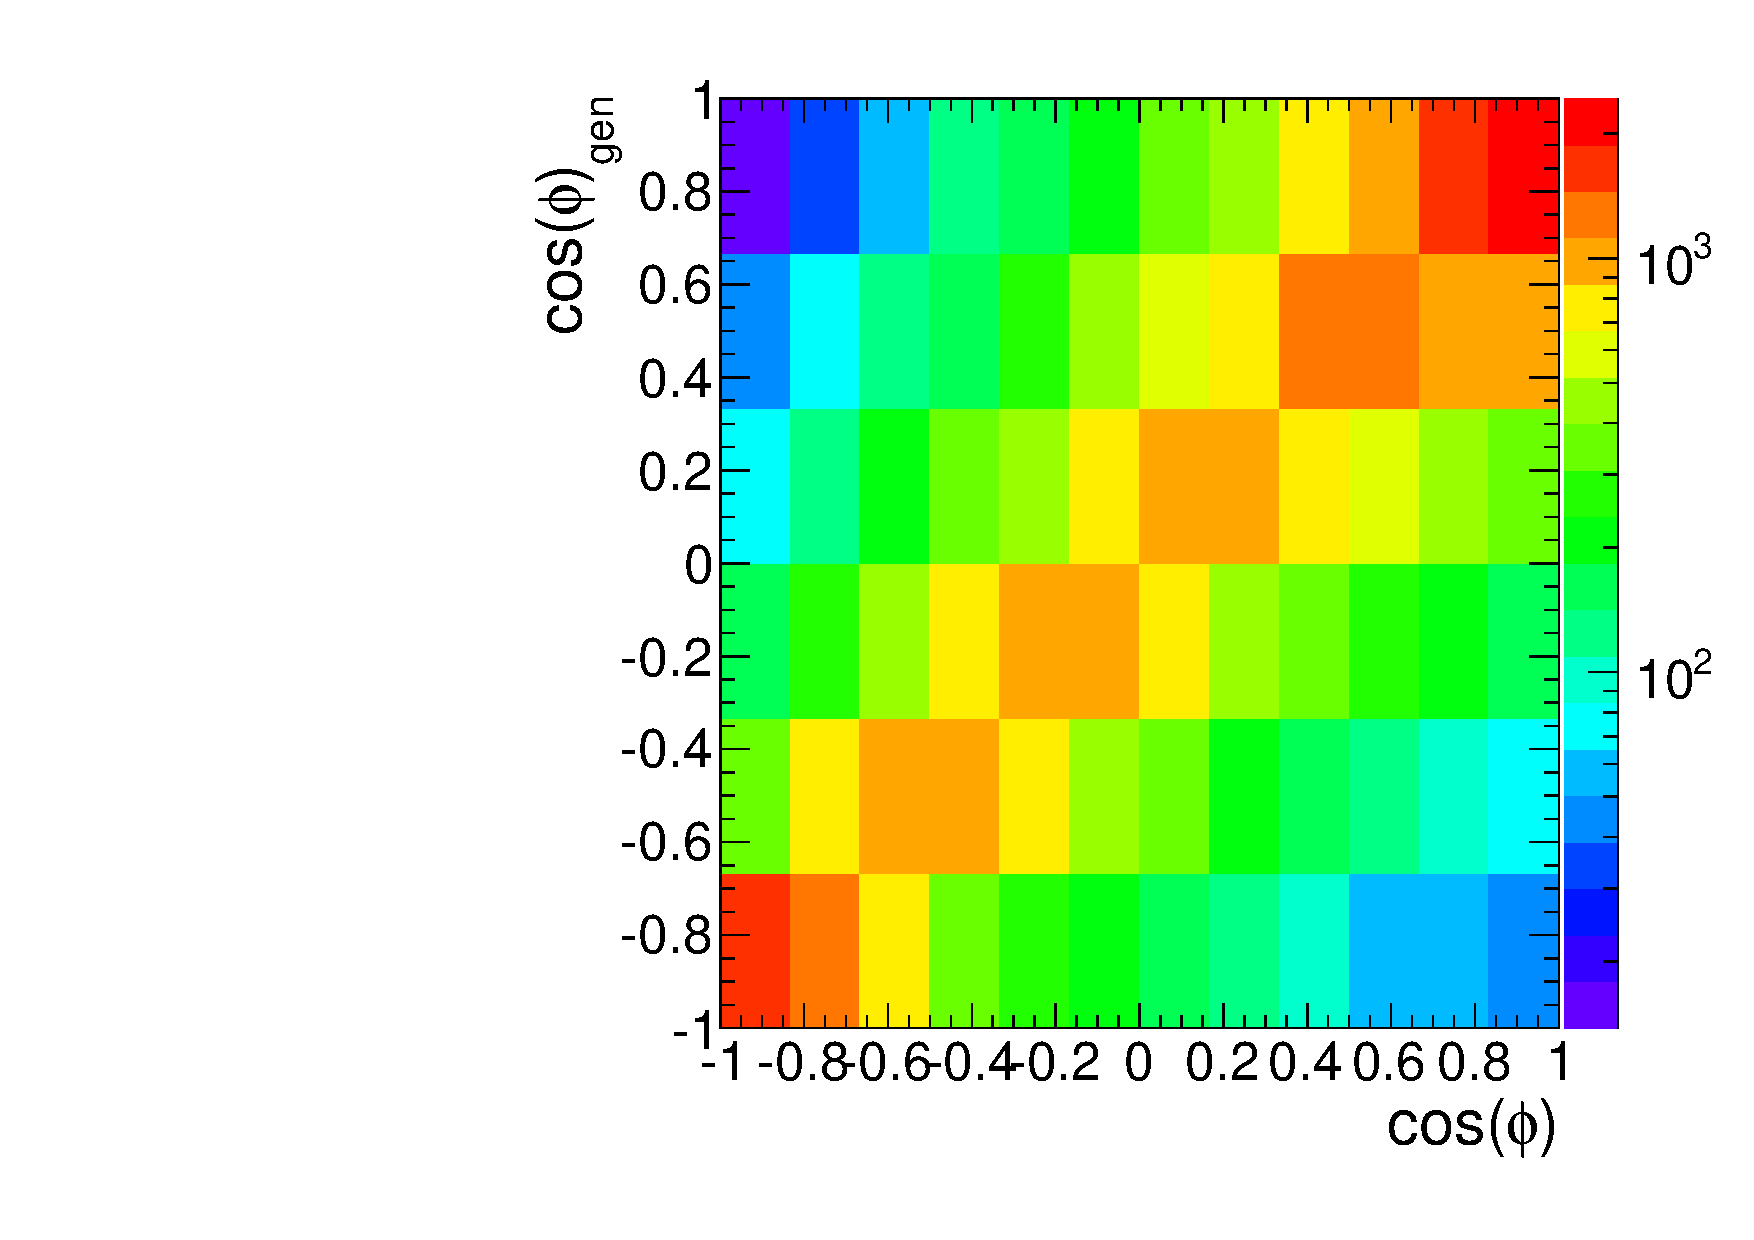
\includegraphics[width=0.325\linewidth]{figures/smearing_lepCosOpeningAngle_all.pdf}
\caption{Smearing matrices for the six asymmetry variables.}
\label{fig:afb:smearing}
\end{figure}

As described in Section \ref{ssec:afb:unfoldingbkg}, the choice of the
regularization strength parameter, $\tau$, will impact both the amount of statistical
fluctuation in the unfolded distribution, and the amount of
bias. There are many ways to choose the optimal value of this parameter. We
use the method of minimizing the mean of the global correlation
coefficients, which is also favored by Blobel
\cite{blobelseminar}. The values of $\tau$ we arrived at in this way
are presented in Table \ref{tab:afb:tau1d}. To validate these values,
we checked how the unfolded asymmetries and their uncertainties varied as we scaled
$\tau$ up and down by up to a factor of 100. As expected, the
uncertainties became larger as $\tau$ was decreased; as $\tau$ was
increased, the asymmetry central value shifted, indicating bias. From
this behavior, we deduce that our choices for $\tau$ were
appropriate. The dependence of the asymmetries and their uncertainties
on the choice of $\tau$ is shown in Figure \ref{fig:afb:tauvary}.

% Table of tau values from AN-14-246. Unpublished. %%%%%%%%%%%%%%%%%%%%%%%%%%%%
\begin{table}[htb]
\begin{center}
\caption{Optimized $\tau$ values chosen for each asymmetry.}
\label{tab:afb:tau1d}
\begin{tabular}{l | c  c  c  c  c  c }
\hline
Asymmetry & $A^{lep}_{C}$ & $A_{\Delta\phi}$ & $A_{C}$ & $A_{P}$ & $A_{c1c2}$ & $A_{\cos\phi}$ \\ \hline
$\tau$ value & 0.000185 & 0.000166 & 0.000110 & 0.000075 & 0.000089 & 0.000098 \\ \hline
\end{tabular}
\end{center}
\end{table}

\begin{figure}[!htpb]
\centering
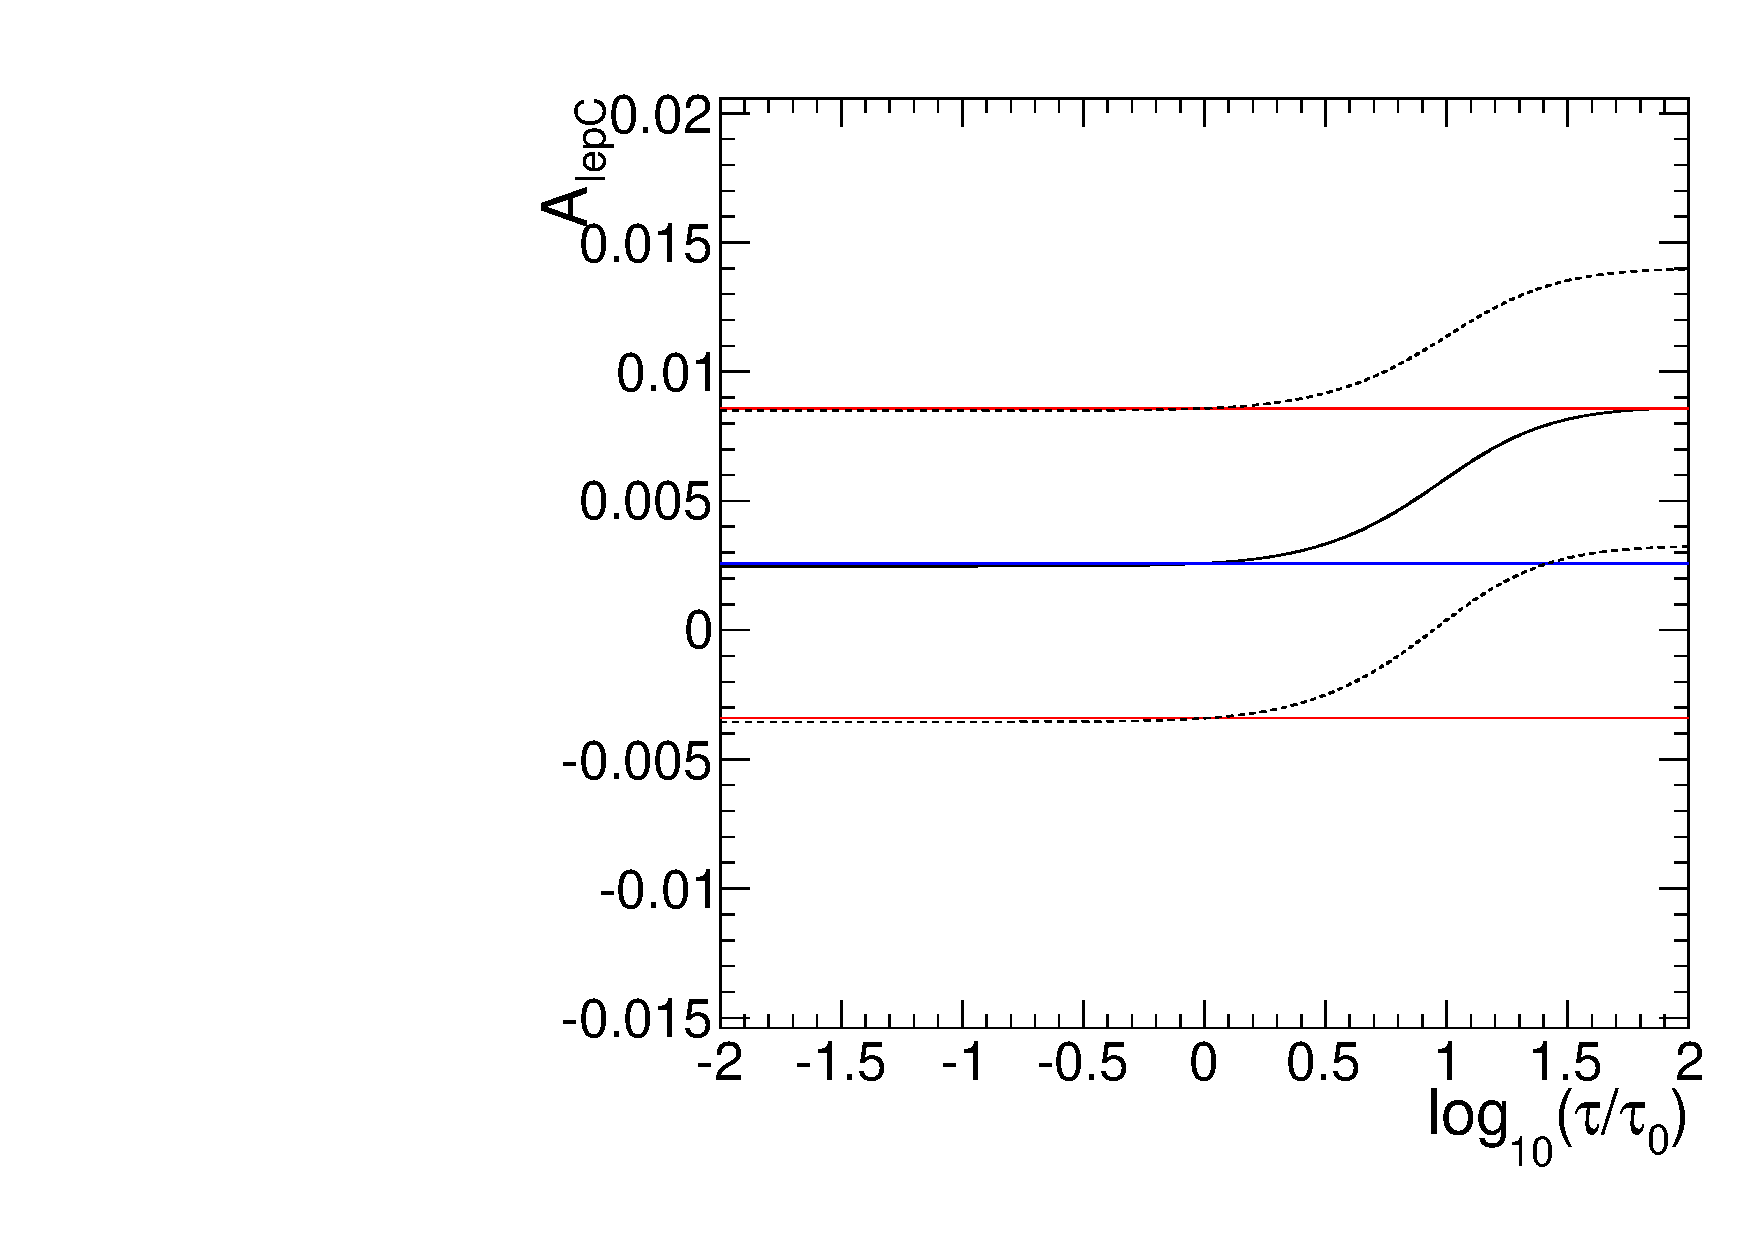
\includegraphics[width=0.325\linewidth]{figures/tau_variation_lepChargeAsym.pdf}
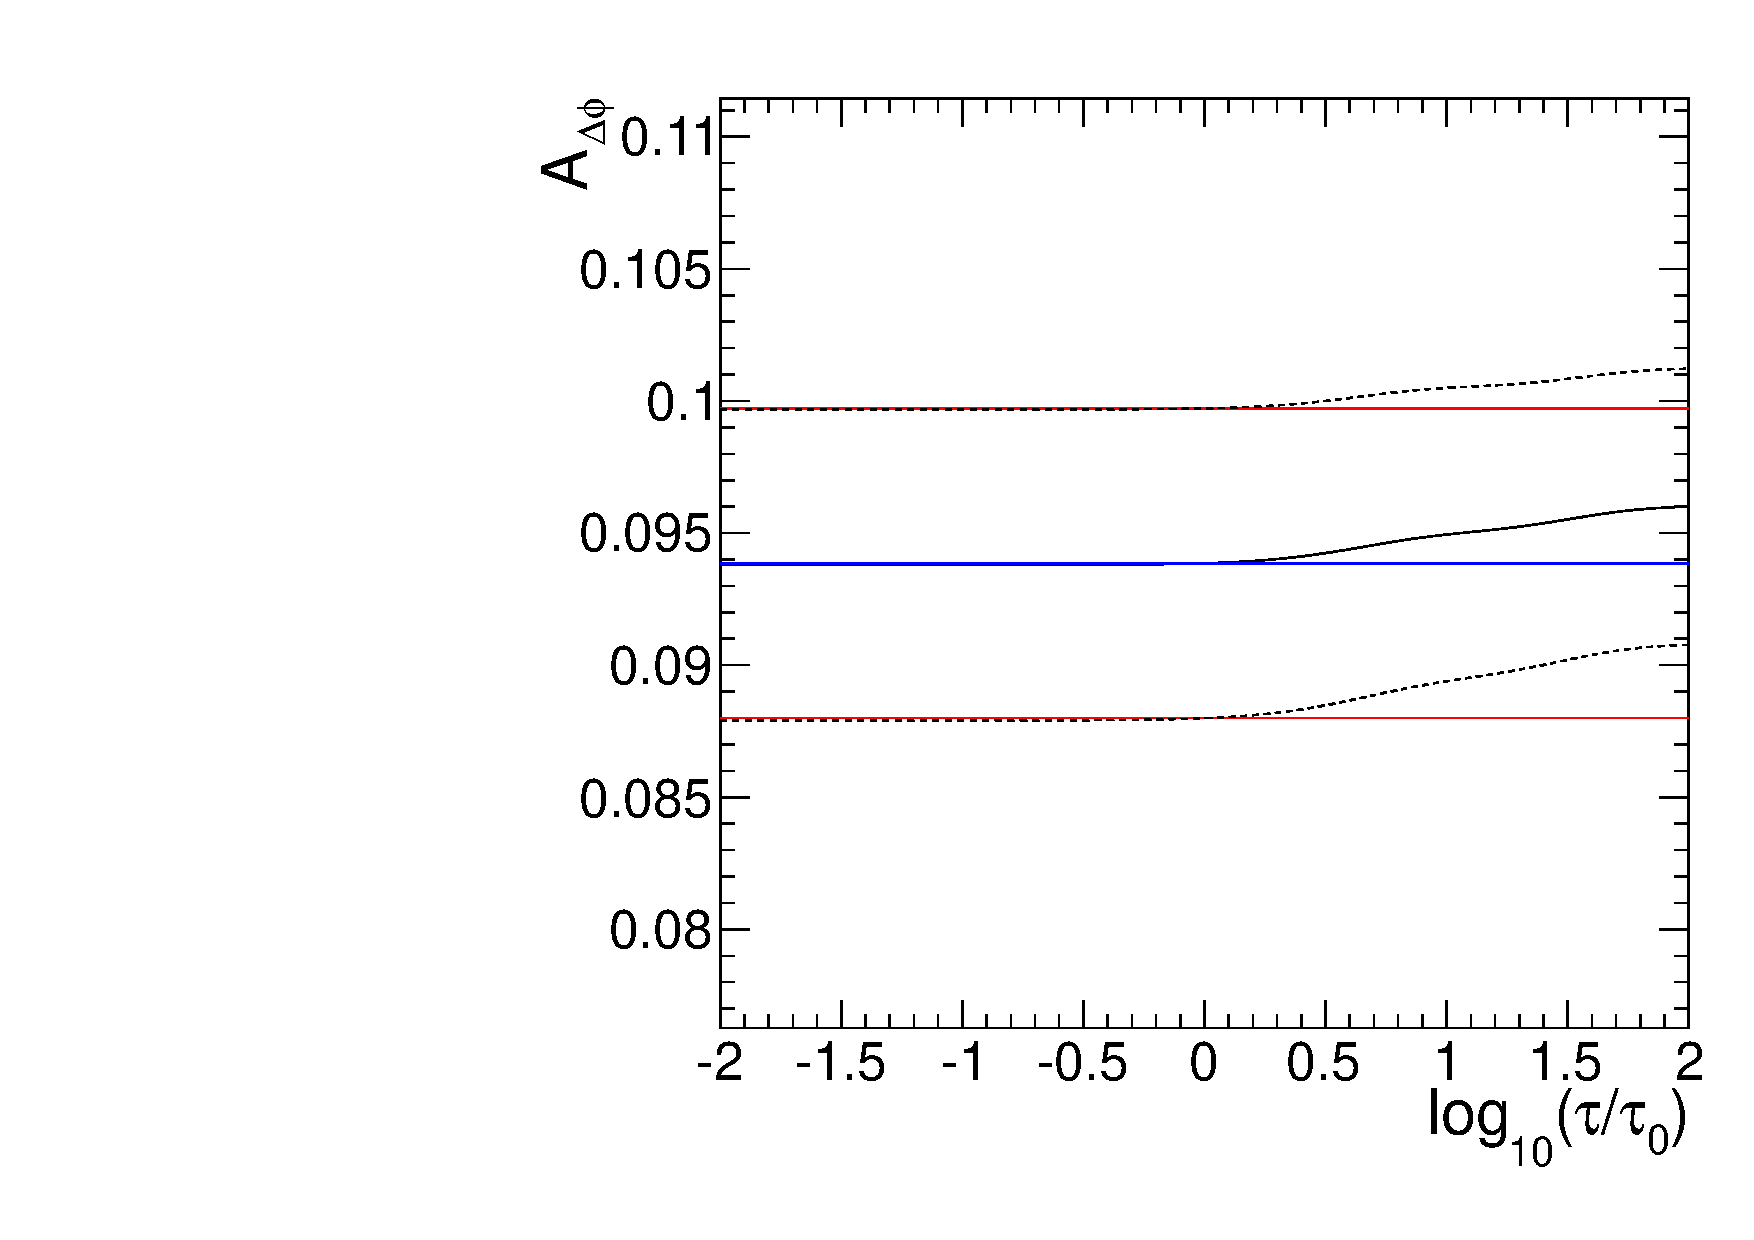
\includegraphics[width=0.325\linewidth]{figures/tau_variation_lepAzimAsym2.pdf}
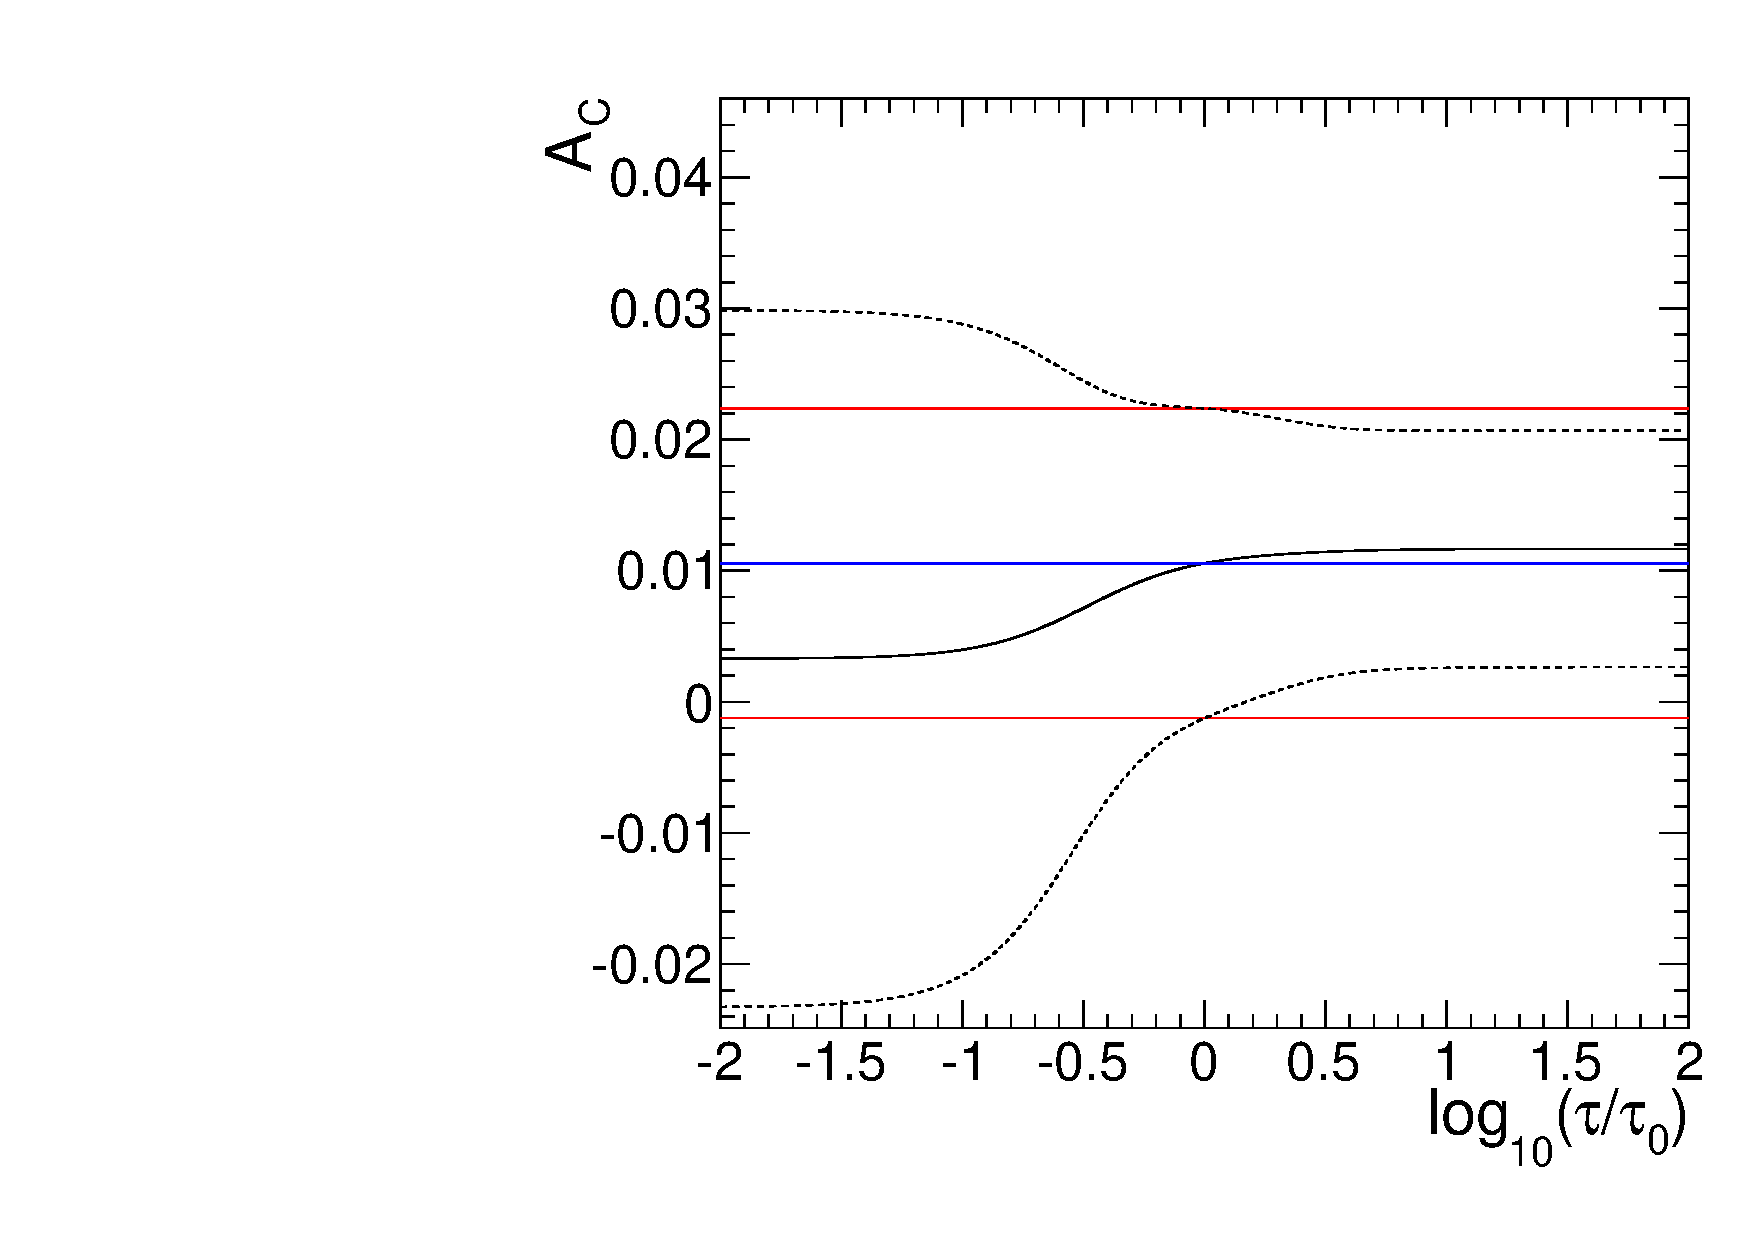
\includegraphics[width=0.325\linewidth]{figures/tau_variation_rapiditydiffMarco.pdf}
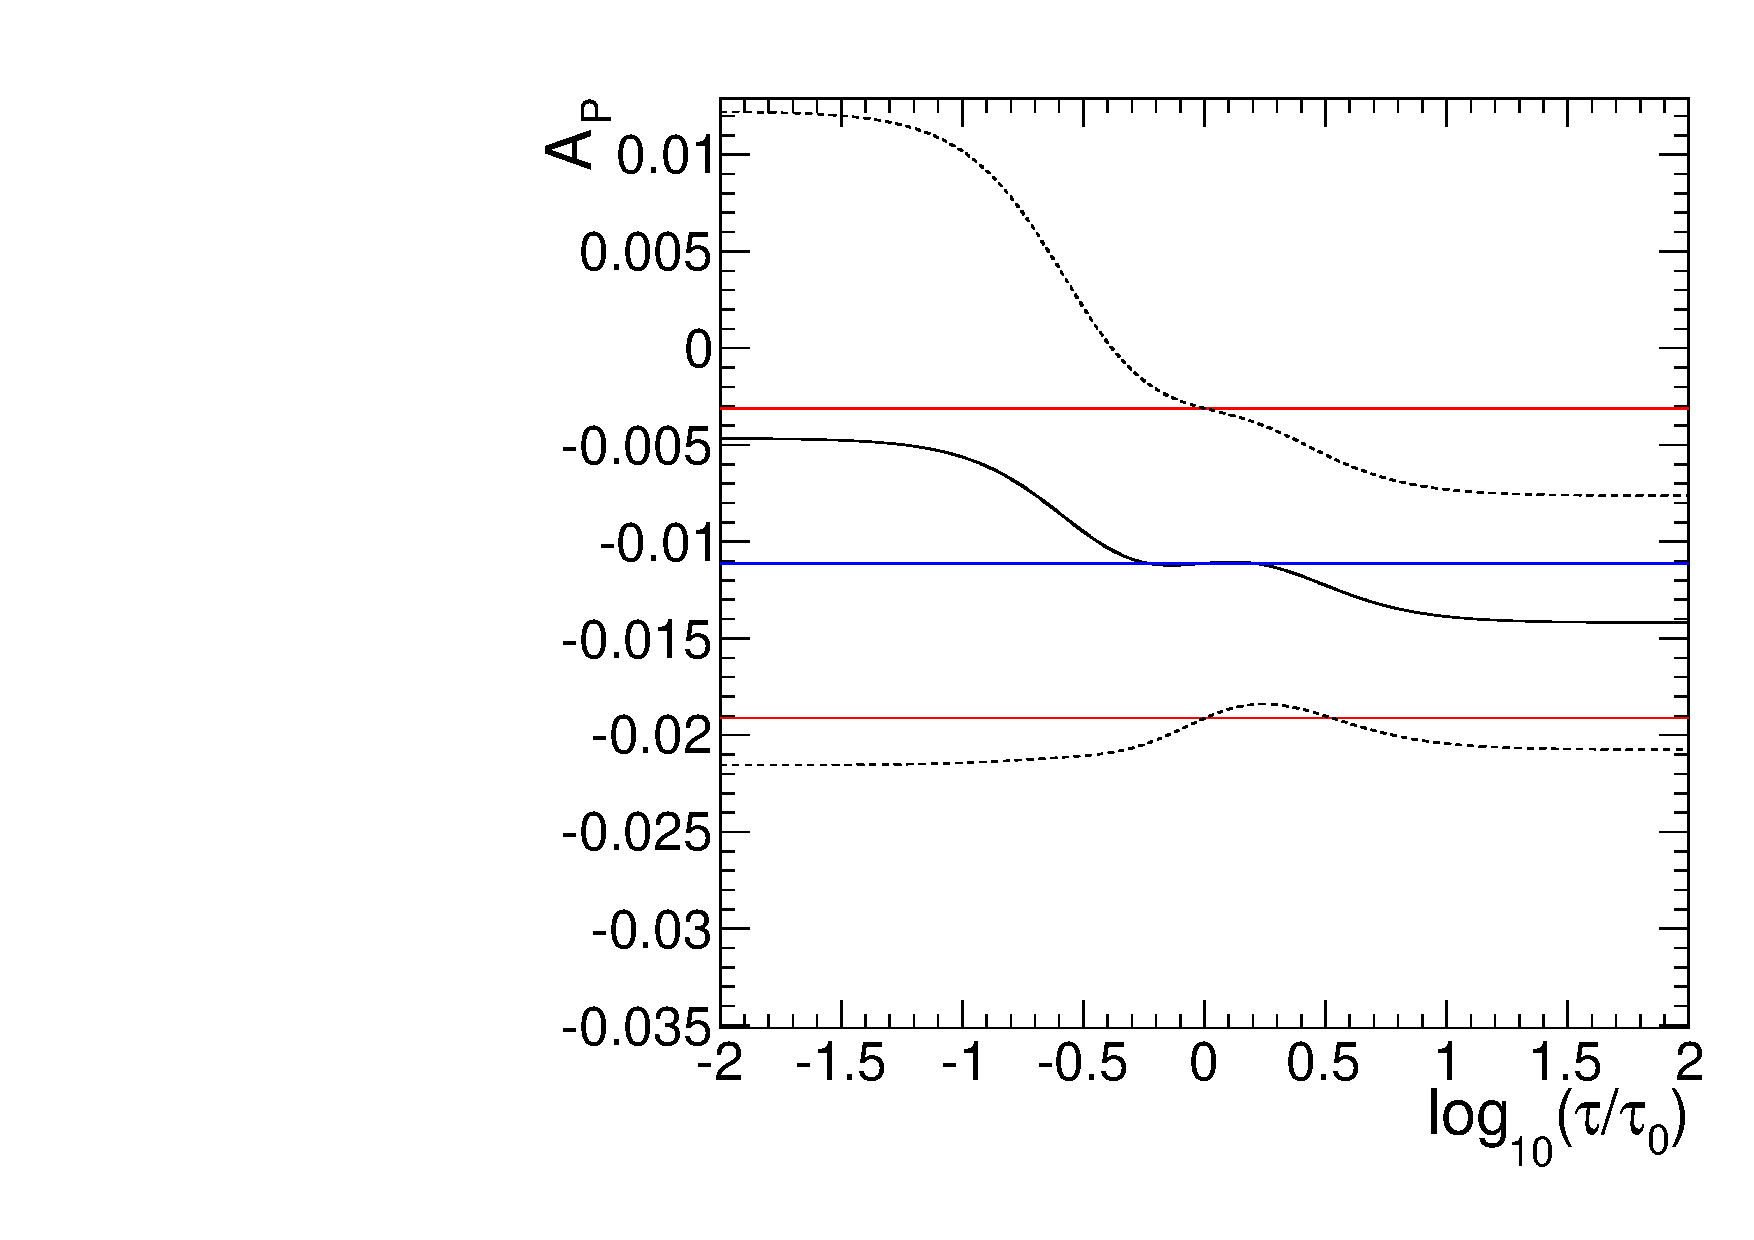
\includegraphics[width=0.325\linewidth]{figures/tau_variation_lepCosTheta.pdf}
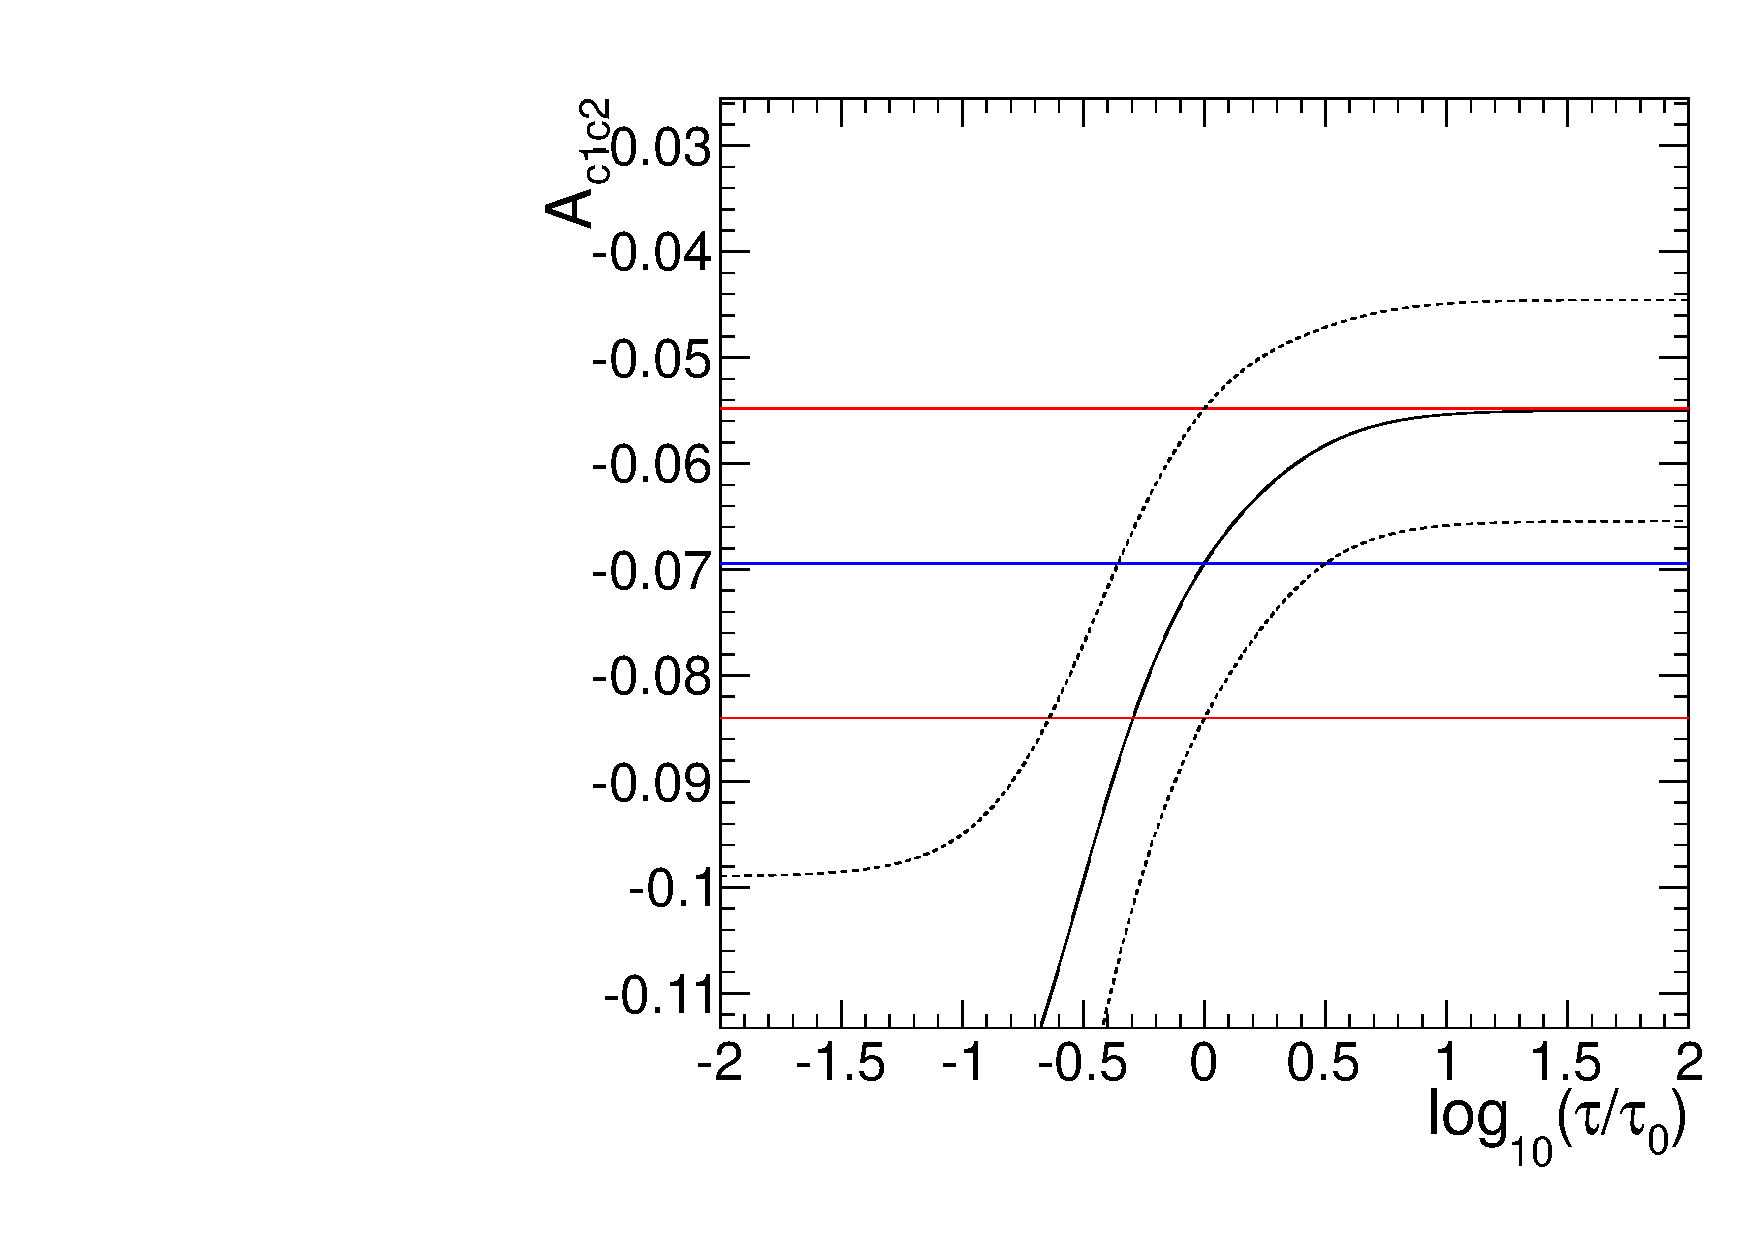
\includegraphics[width=0.325\linewidth]{figures/tau_variation_topSpinCorr.pdf}
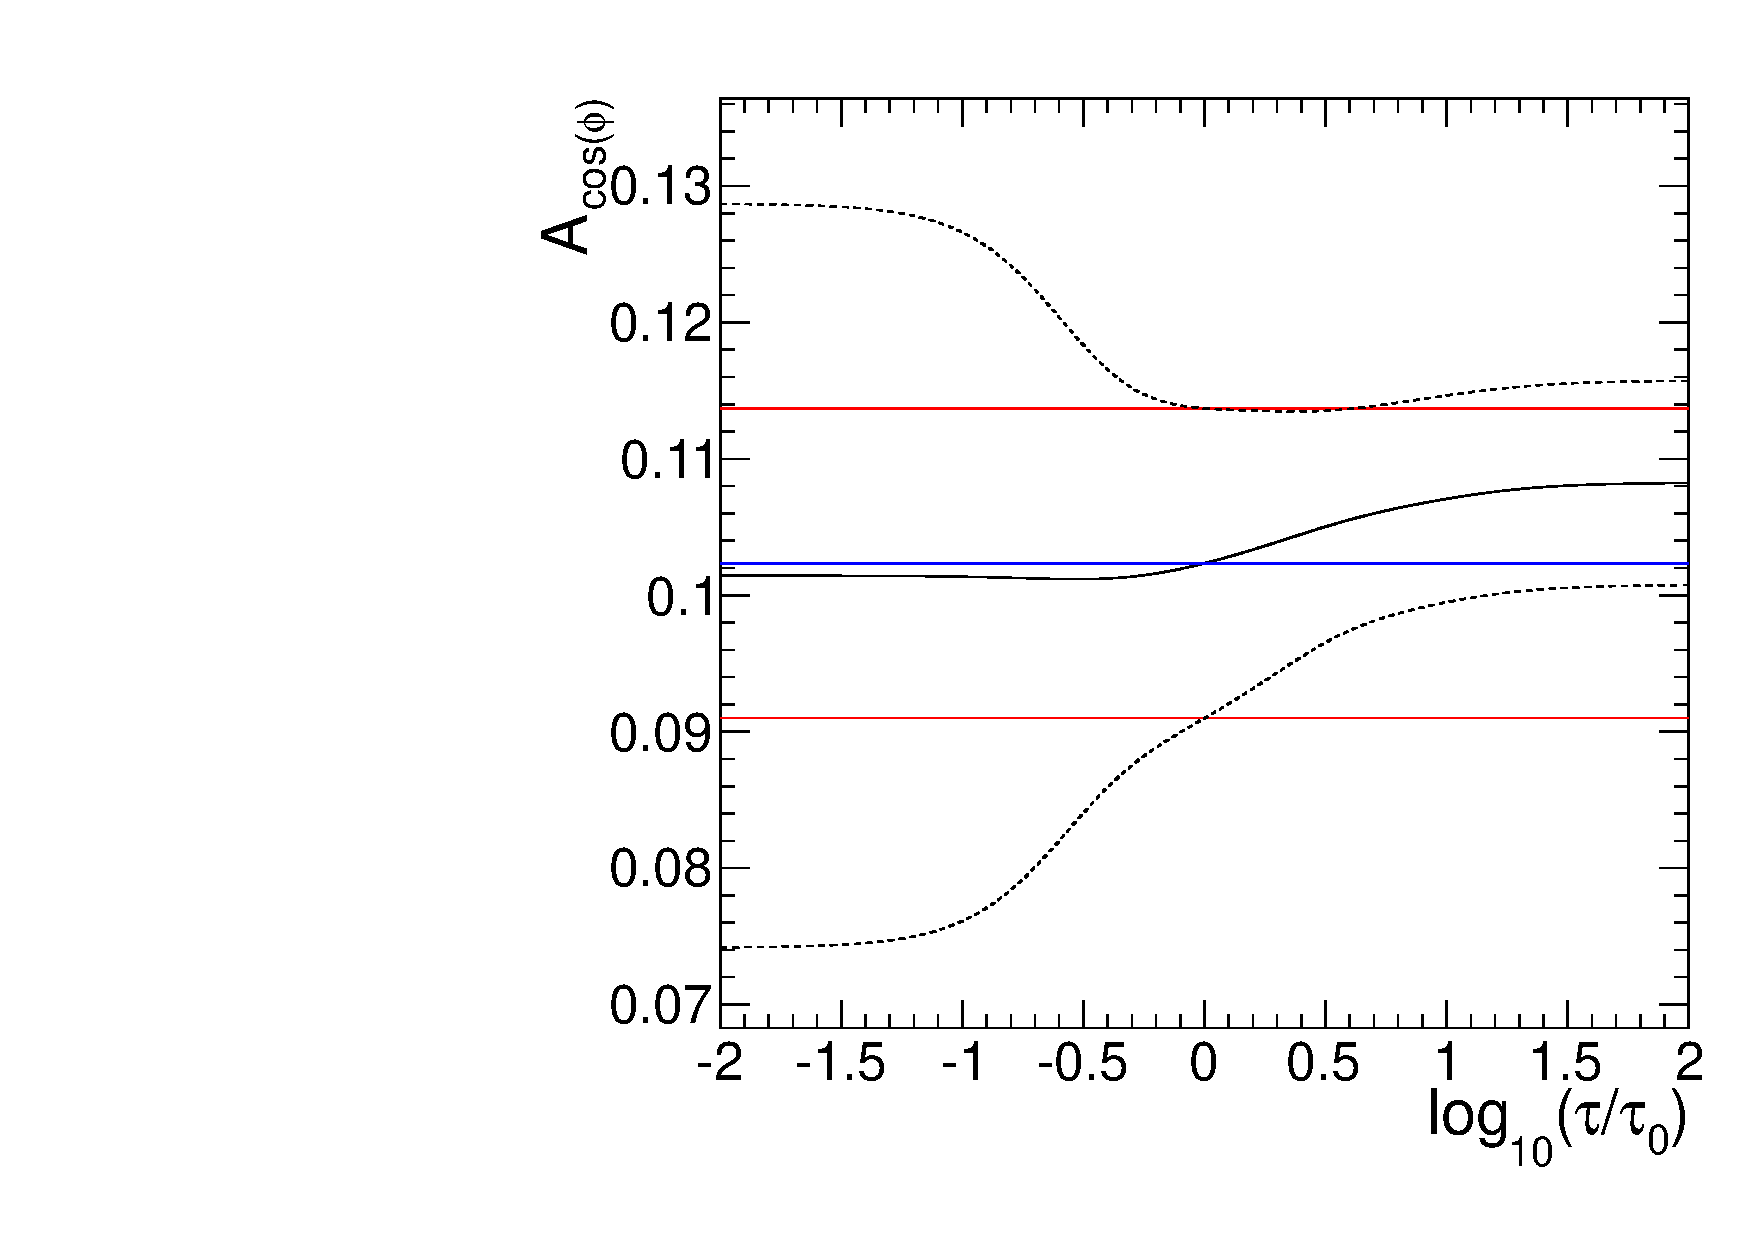
\includegraphics[width=0.325\linewidth]{figures/tau_variation_lepCosOpeningAngle.pdf}
\caption{Dependence of unfolded asymmetries and uncertainties on
  the regularization strength, $\tau$. Blue lines denote the
  nominal unfolded asymmetry, and red lines denote the nominal
  uncertainty bounds. Black lines show how these values vary with $\tau$.}
\label{fig:afb:tauvary}
\end{figure}

We performed the actual regularized unfolding using the TUnfold
package \cite{tunfold}. We chose TUnfold because it provides good
support for two-dimensional unfolding, a process described in the next
section. The results of the one-dimensional unfolding are presented in
Section \ref{ssec:afb:results1d}. The tests for bias due to
regularization are presented in Section \ref{ssec:afb:unfoldingtests}.

\subsection{Two-Dimensional Unfolding Procedure}
\label{ssec:afb:unfolding2d}

As described in Section \ref{ssec:afb:varsdifferential}, we also wish
to measure our asymmetries differentially with respect to three
different kinematic variables -- the mass, absolute rapidity, and transverse
momentum of the $\ttbar$ system. For our asymmetry variables, we use
the same binning described in Table \ref{tab:afb:binning1d}. For the
secondary variables, our chosen binning is described in Table
\ref{tab:afb:binning2d}.

% Binning table from AN-14-246. Believed unpublished, but could probably be deduced from published plots.
\begin{table}[htb]
\begin{center}
\caption{Bins chosen for kinematic variables in differential measurements.}
\label{tab:afb:binning2d}
\begin{tabular}{l |  c  c  c }
\hline
Secondary Variable &  B1  &  B2 &  B3 \\ \hline
$m_{\ttbar}$ (GeV)    &  [0, 430]  &  [430,530]  &  [530,$\infty$]  \\ \hline
$p_{T}^{\ttbar}$ (GeV)    &  [0,41]  &  [41,92]  &  [92,$\infty$] \\ \hline
$|y_{\ttbar}|$        &  [0,0.34]  &  [0.34,0.75]  &  [0.75,$\infty$] \\ \hline
 \hline
\end{tabular}
\end{center}
\end{table}

The procedure for unfolding these two-dimensional distributions is
nearly identical to the procedure for unfolding
one-dimensional distributions. We convert our two-dimensional
distributions into one-dimensional distributions by essentially
``unwrapping'' the 2D histogram into a 1D histogram. If the 2D
histogram has the familiar 6(12) bins on the x-axis, and 3 rows (i.e. bins) on the
y-axis, we concatenate those three rows together to form a 1D histogram
(a single row) with 18(36) bins. We can then unfold the unwrapped
distribution, and re-wrap it to obtain the differential asymmetry
measurements. The correspondence between the wrapped and unwrapped
histograms is shown in Figure \ref{fig:afb:unwrapping}.

% Figure I made myself to show how the unwrapping works, and how
% regularizing adjacent bins becomes complicated
\begin{figure}[htb]
\centering
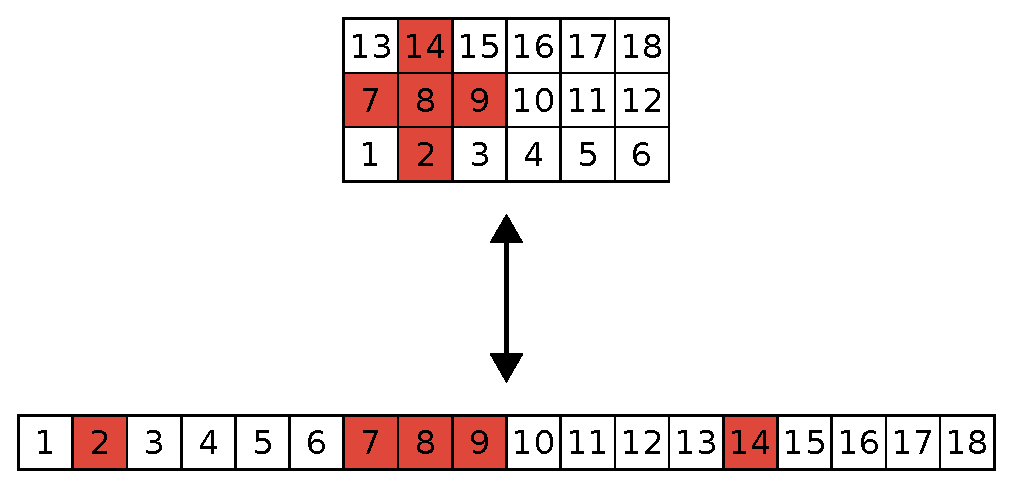
\includegraphics[width=0.9\textwidth]{figures/unwrapping.pdf}
\caption{Comparison between wrapped 2D histogram and unwrapped 1D
  histogram. Each numbered box corresponds to a histogram bin. Bin
  8 and its adjacent bins are highlighted in red to illustrate how
  adjacency is not always preserved by the unwrapping process.}
\label{fig:afb:unwrapping}
\end{figure}

The smearing and acceptance matrices used for unfolding in two
dimensions follow this same unwrapping scheme, but are otherwise
derived identically to those for 1D unfolding.
% Interestingly, the smearing matrices based on unwrapped distributions
% show a $3 \times 3$ structure that comes from migration between bins
% in the kinematic variable.
The regularization parameter $\tau$ is chosen for 2D unfolding just as
it was for 1D unfolding, by finding the value that minimizes the mean
of the global correlation coefficients. As an example, the $\tau$
values used for 2D unfolding vs. $m_{\ttbar}$ are given in Table
\ref{tab:afb:tau2d}.

% Table of 2D tau values vs Mttbar from AN-14-246. Unpublished.
\begin{table}[htbp]
\begin{center}
\caption{Optimized $\tau$ values used to unfold each asymmetry
  differentially with respect to $m_{\ttbar}.$}
\label{tab:afb:tau2d}
\begin{tabular}{l | c  c  c  c  c  c }
\hline
Asymmetry & $A^{lep}_{C}$ & $A_{\Delta\phi}$ & $A_{C}$ & $A_{P}$ & $A_{c1c2}$ & $A_{\phi}$ \\ \hline
$\tau$ value & 0.000426 & 0.000422 & 0.000144 & 0.000102 & 0.000120 & 0.000121 \\ \hline
\end{tabular}
\end{center}
\end{table}

Our regularization procedure was already described in Section
\ref{ssec:afb:unfoldingbkg}, however there is an additional subtlety
introduced in two-dimensional unfolding. Because the distribution we
are unfolding is actually an ``unwrapped'' two-dimensional
distribution, we do not want to regularize the curvature at the
boundaries between unwrapped rows. In addition, we also wish to
regularize in the secondary variable, which, in the unwrapped
distribution, means we must regularize bins that are no longer
adjacent. Using Figure \ref{fig:afb:unwrapping} as an example, bin 8
must be regularized with bins 7, 9, 2, and 14; however, bins 12 and 13
must not be regularized with each other.
We specifically chose to use TUnfold because it natively supports such
complex regularization schemes \cite{tunfold}. The results of the 2D unfolding
procedure are presented in Section \ref{ssec:afb:results2d}, and the
bias tests are described in the next section.

\subsection{Linearity Tests}
\label{ssec:afb:unfoldingtests}

As described in Section \ref{ssec:afb:unfoldingbkg}, regularization
introduces some amount of bias to our unfolded results because it
forces the results to take on characteristics of a distribution
we supply. But since regularization is important for
controlling statistical fluctuations in the output, we cannot abandon
it entirely. We must therefore try to quantify the amount of bias
introduced by regularization, and judge whether or not it is acceptable.

To test the amount of bias introduced by regularization, we perform
\emph{linearity tests} on our asymmetries. For each asymmetry, we
begin by reweighting the $\ttdilep$ Monte Carlo events using a linear
function of the measured variable. For example, Equation
\ref{eq:afb:topchargeasym} describes the top charge asymmetry in terms
of the measured variable $|y_t| - |y_{\bar{t}}|$, so the reweighting
equation would be:
\begin{equation}
\text{weight} = 1 + K \cdot (|y_t| - |y_{\bar{t}}|)
\end{equation}
For other asymmetries, substitute the appropriate measured variable
into this expression. The parameter $K$ is varied between -0.3 and 0.3
in steps of 0.1. This reweighting artificially induces asymmetries of up to
25\% in the simulated data, which is much larger than anything we
would expect from Standard Model or BSM physics.

For each $K$ value, we then make 10,000 copies of the measurement
histogram, and in each copy we fluctuate the various bin contents randomly up and down according to
Poisson statistics. Each of these fluctuated histograms is called a
\emph{pseudoexperiment}, because the Poisson fluctuation approximates
what we might see if we ran our experiment again. Each of
the 10,000 pseudoexperiments is unfolded, and we compare the average
of those unfolded asymmetries against the original,
artificially-induced asymmetry. Figure \ref{fig:afb:linearity}
shows plots of the average unfolded asymmetry vs. the induced asymmetry
for each of the seven $K$ values. We fit these plots
with a straight line, and record the slope and offset
(or intercept) of the line. The slope tells us by what
factor any asymmetry in the data will be scaled up or down by
regularization. On top of that, the offset tells us how much asymmetry
will be added or subtracted by the regularization. These slopes and
offsets are listed in Table \ref{tab:afb:linearity}. Most of the offsets are
zero (the largest is 0.2\%), meaning regularization will add
essentially zero asymmetry that isn't there. The slopes are all
close to 1.0, meaning regularization will not enhance or reduce any
asymmetry in our data by any appreciable amount. The largest slope is 1.024 for
$A_{c1c2}$, meaning this asymmetry could be exaggerated by up to
2.4\% by regularization. We consider this an acceptably small amount
of bias. This information is also taken into consideration when
evaluating our systematic uncertainty due to regularization, described
in Section \ref{sec:afb:systematics}.

% Plots of the linearity results taken from AN-14-246. Unpublished.
\begin{figure}[htpb]
\centering
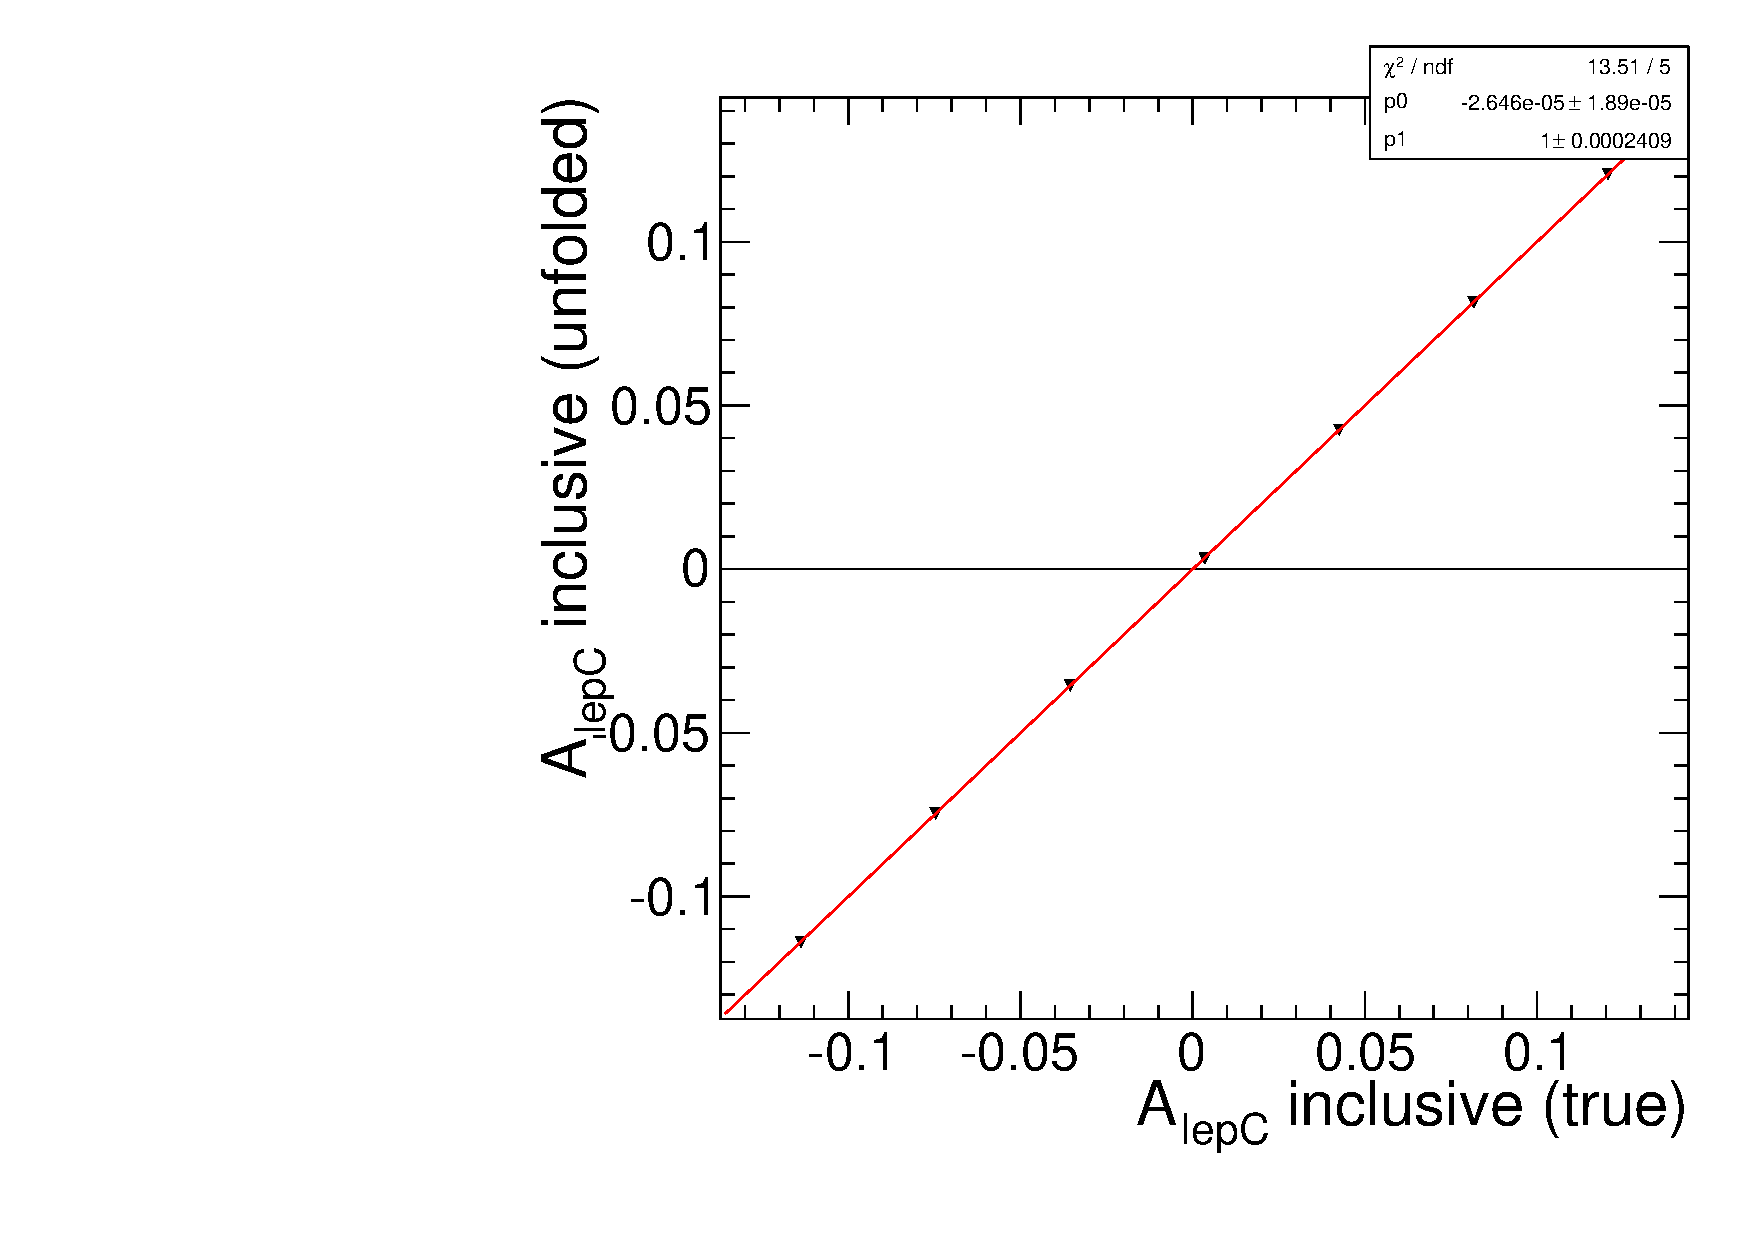
\includegraphics[width=0.325\linewidth]{figures/linearity_lepChargeAsym.pdf}
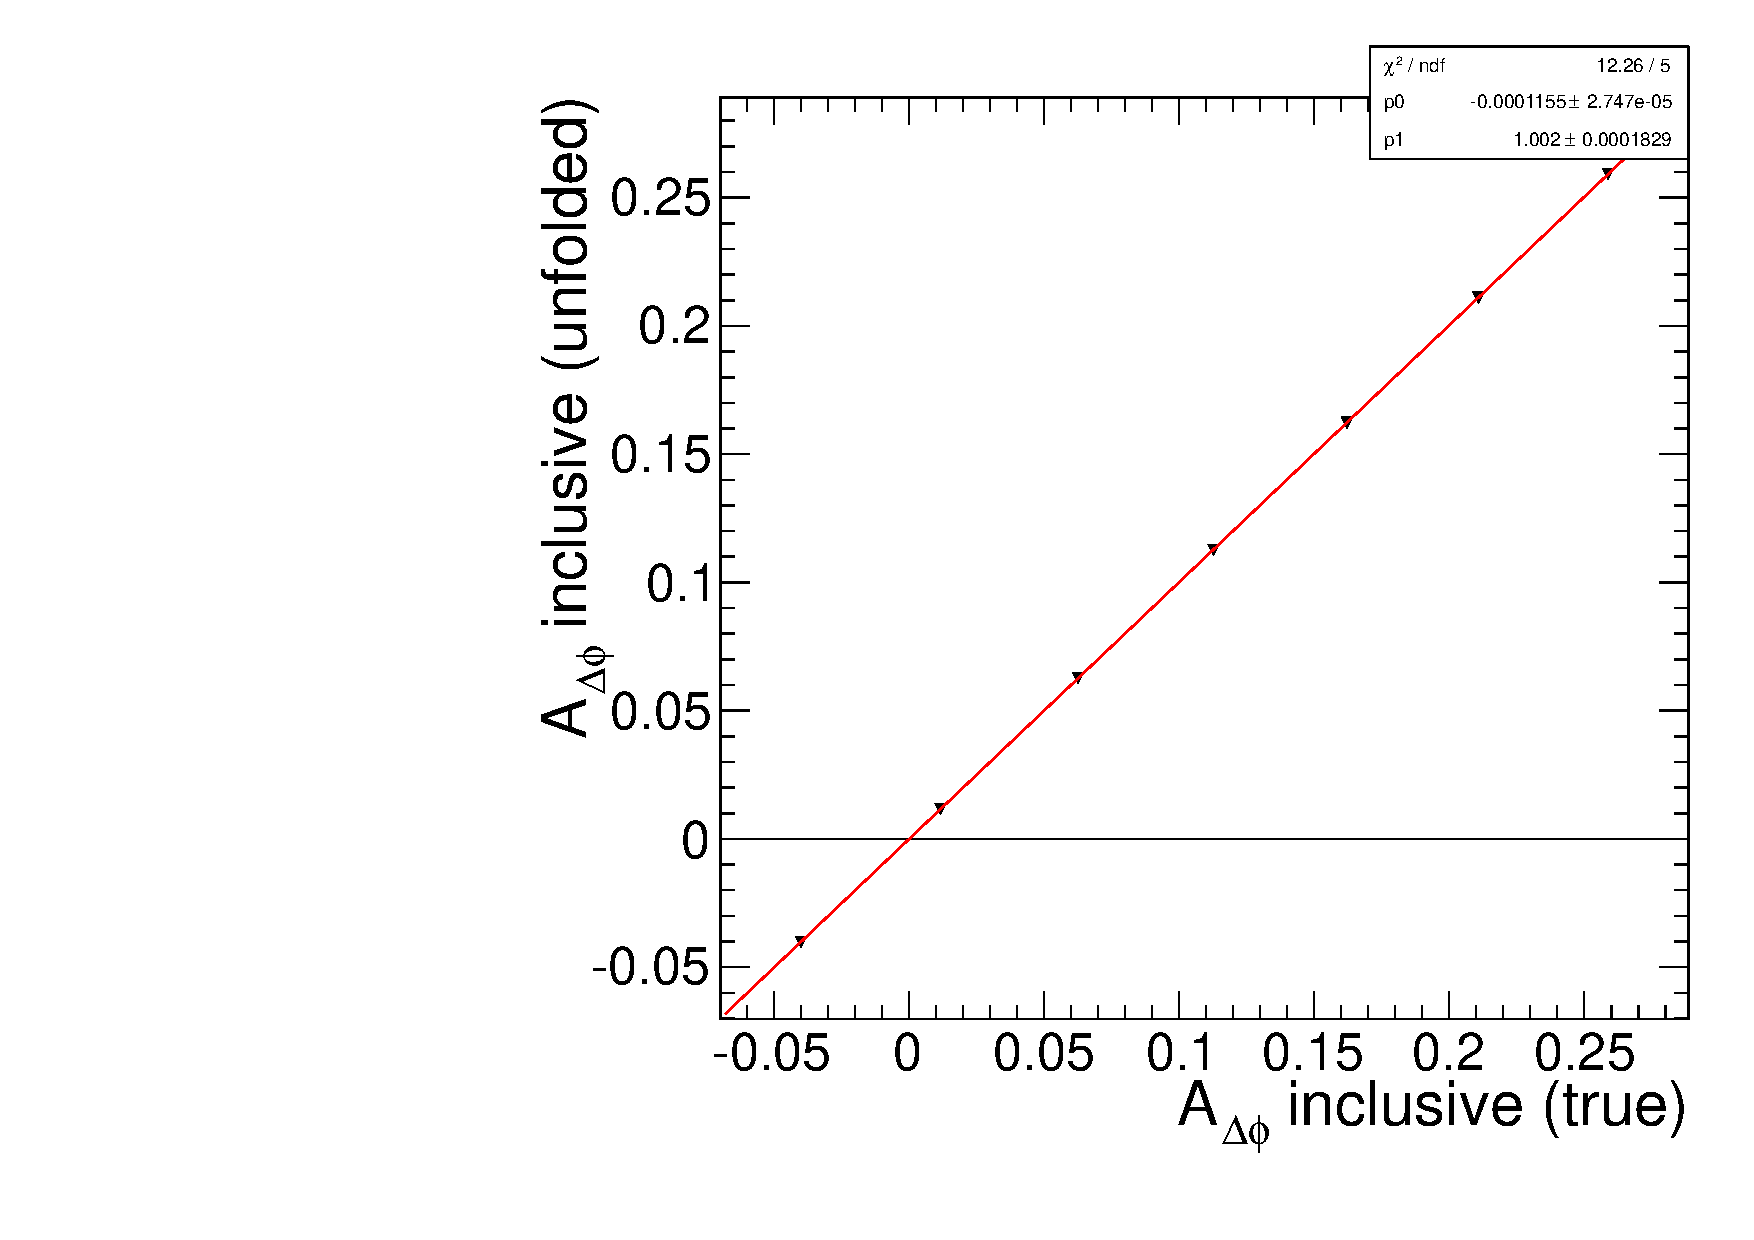
\includegraphics[width=0.325\linewidth]{figures/linearity_lepAzimAsym2.pdf}
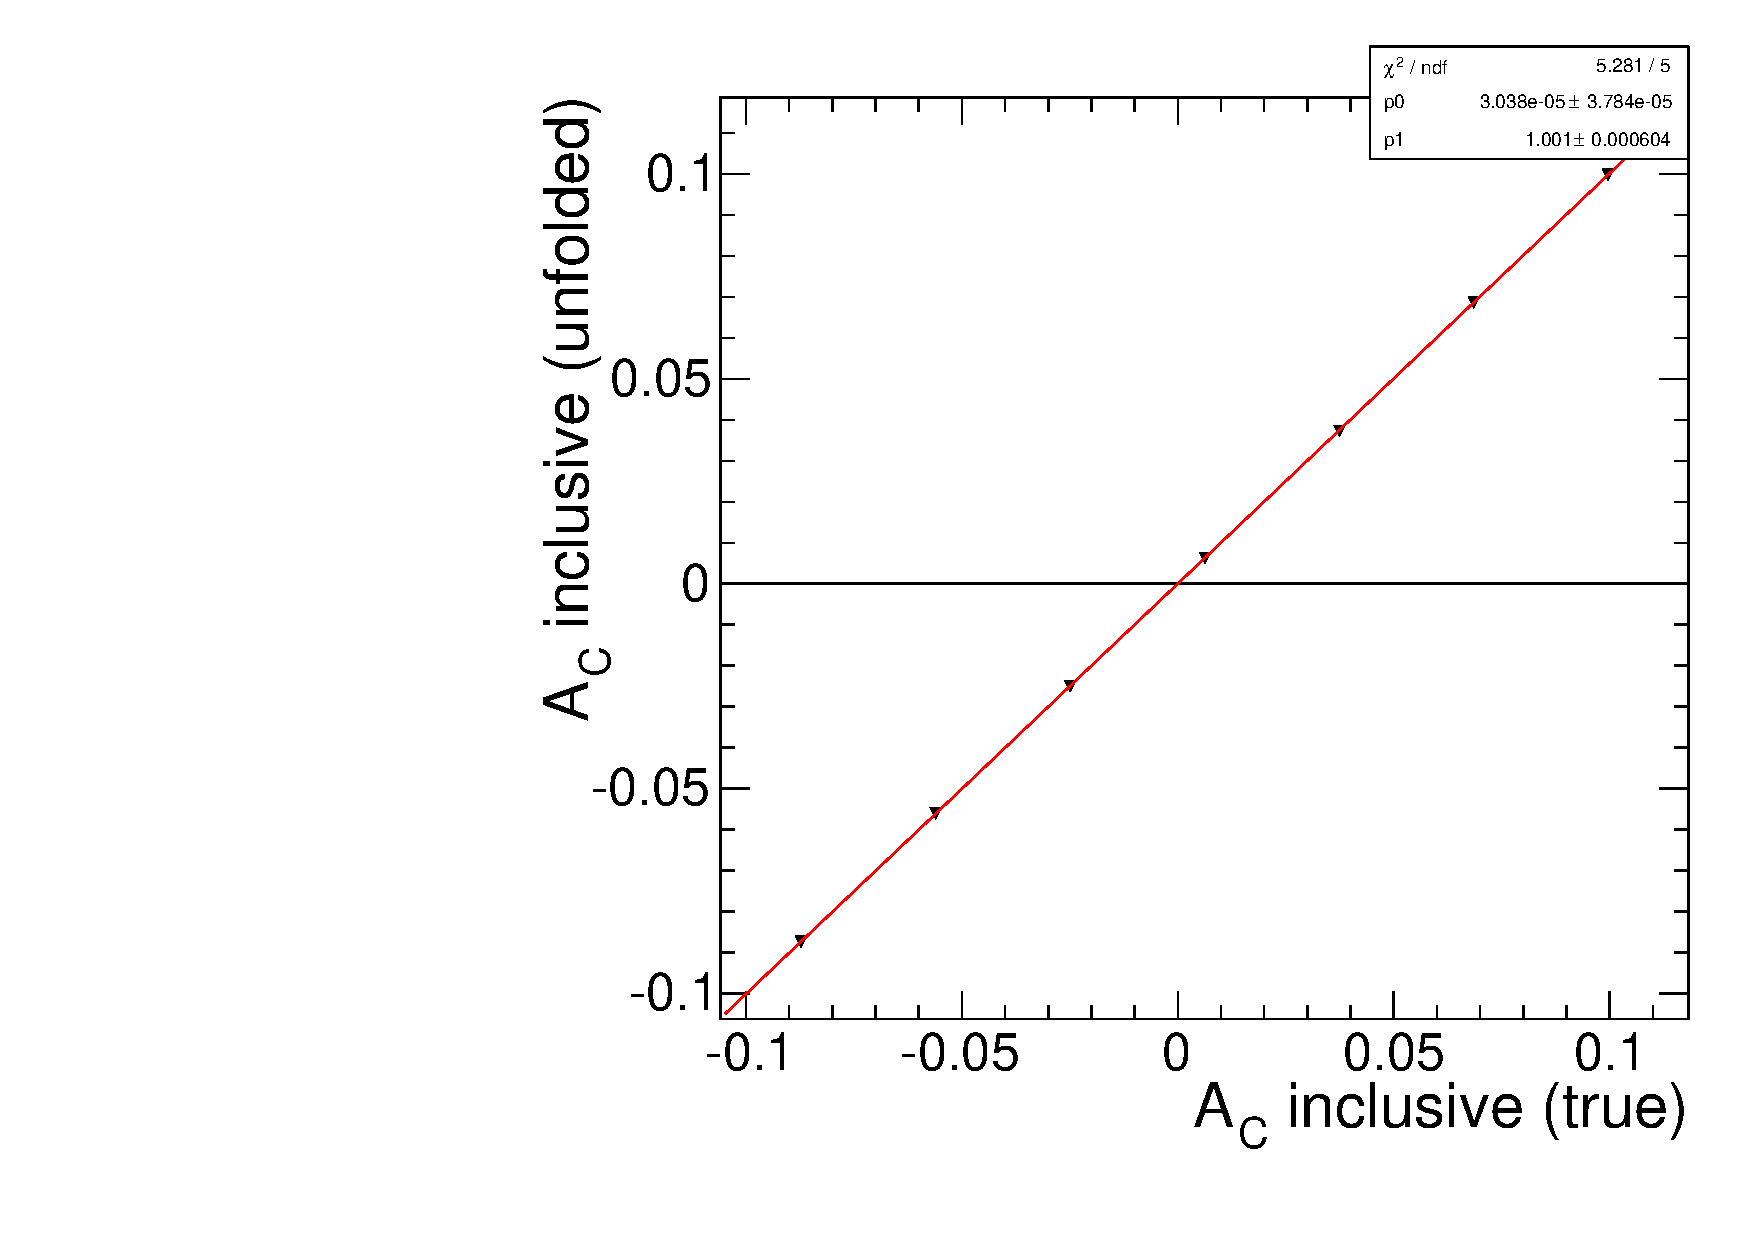
\includegraphics[width=0.325\linewidth]{figures/linearity_rapiditydiffMarco.pdf}
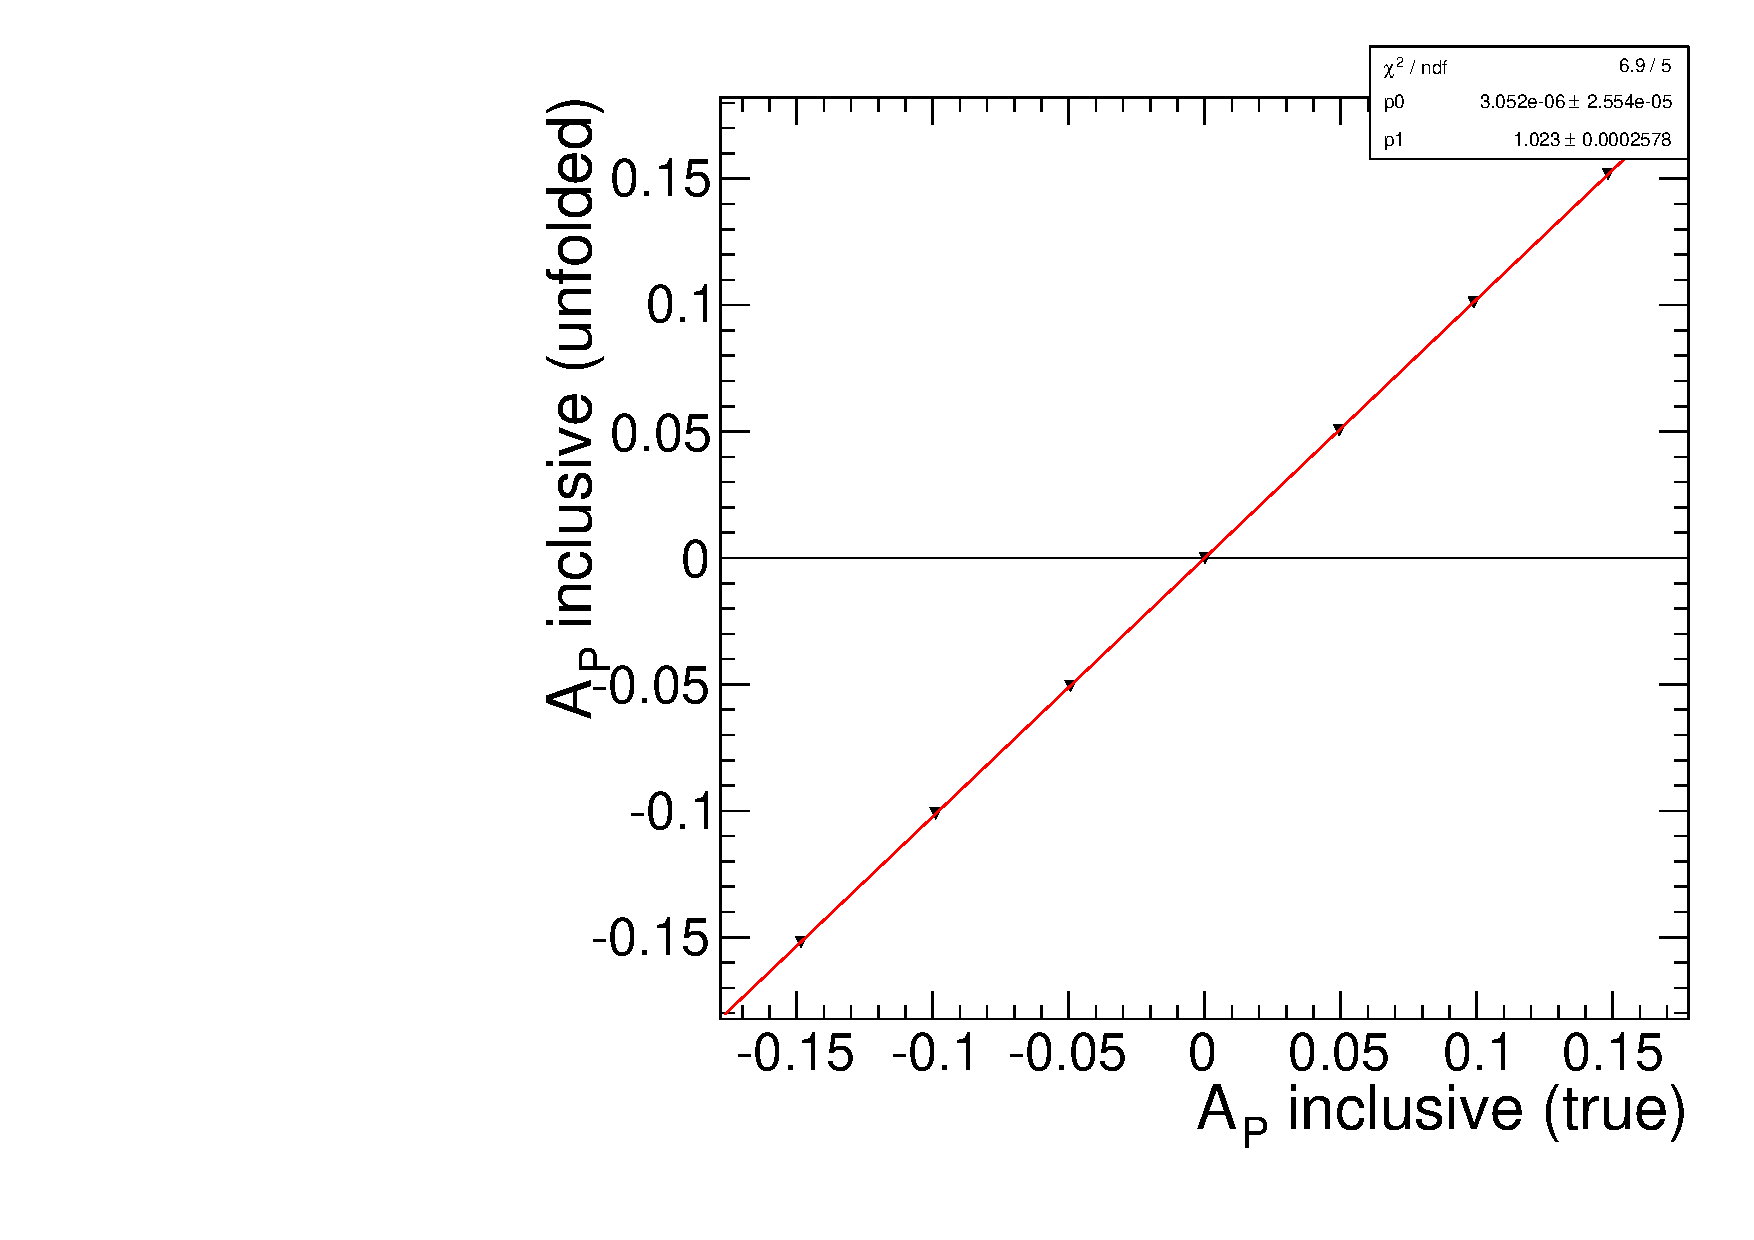
\includegraphics[width=0.325\linewidth]{figures/linearity_lepCosTheta.pdf}
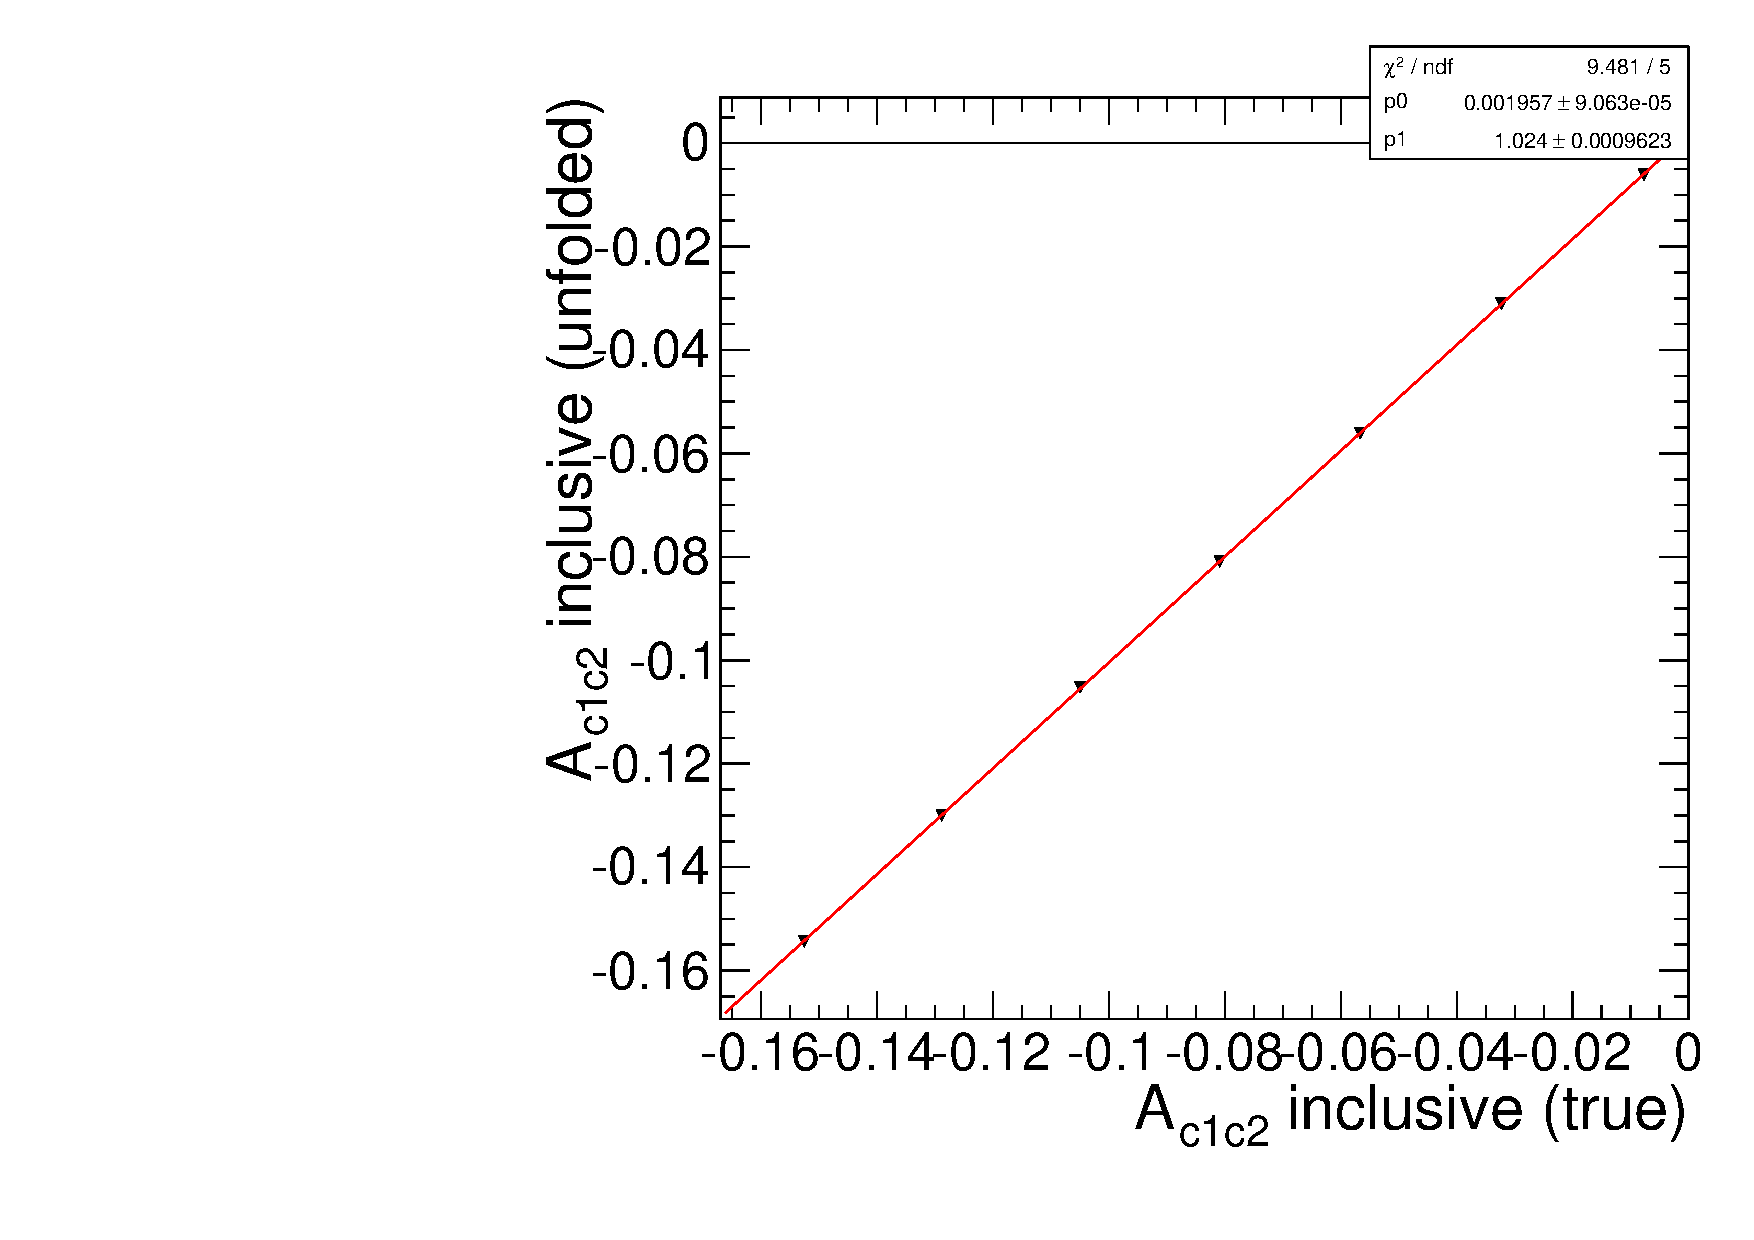
\includegraphics[width=0.325\linewidth]{figures/linearity_topSpinCorr.pdf}
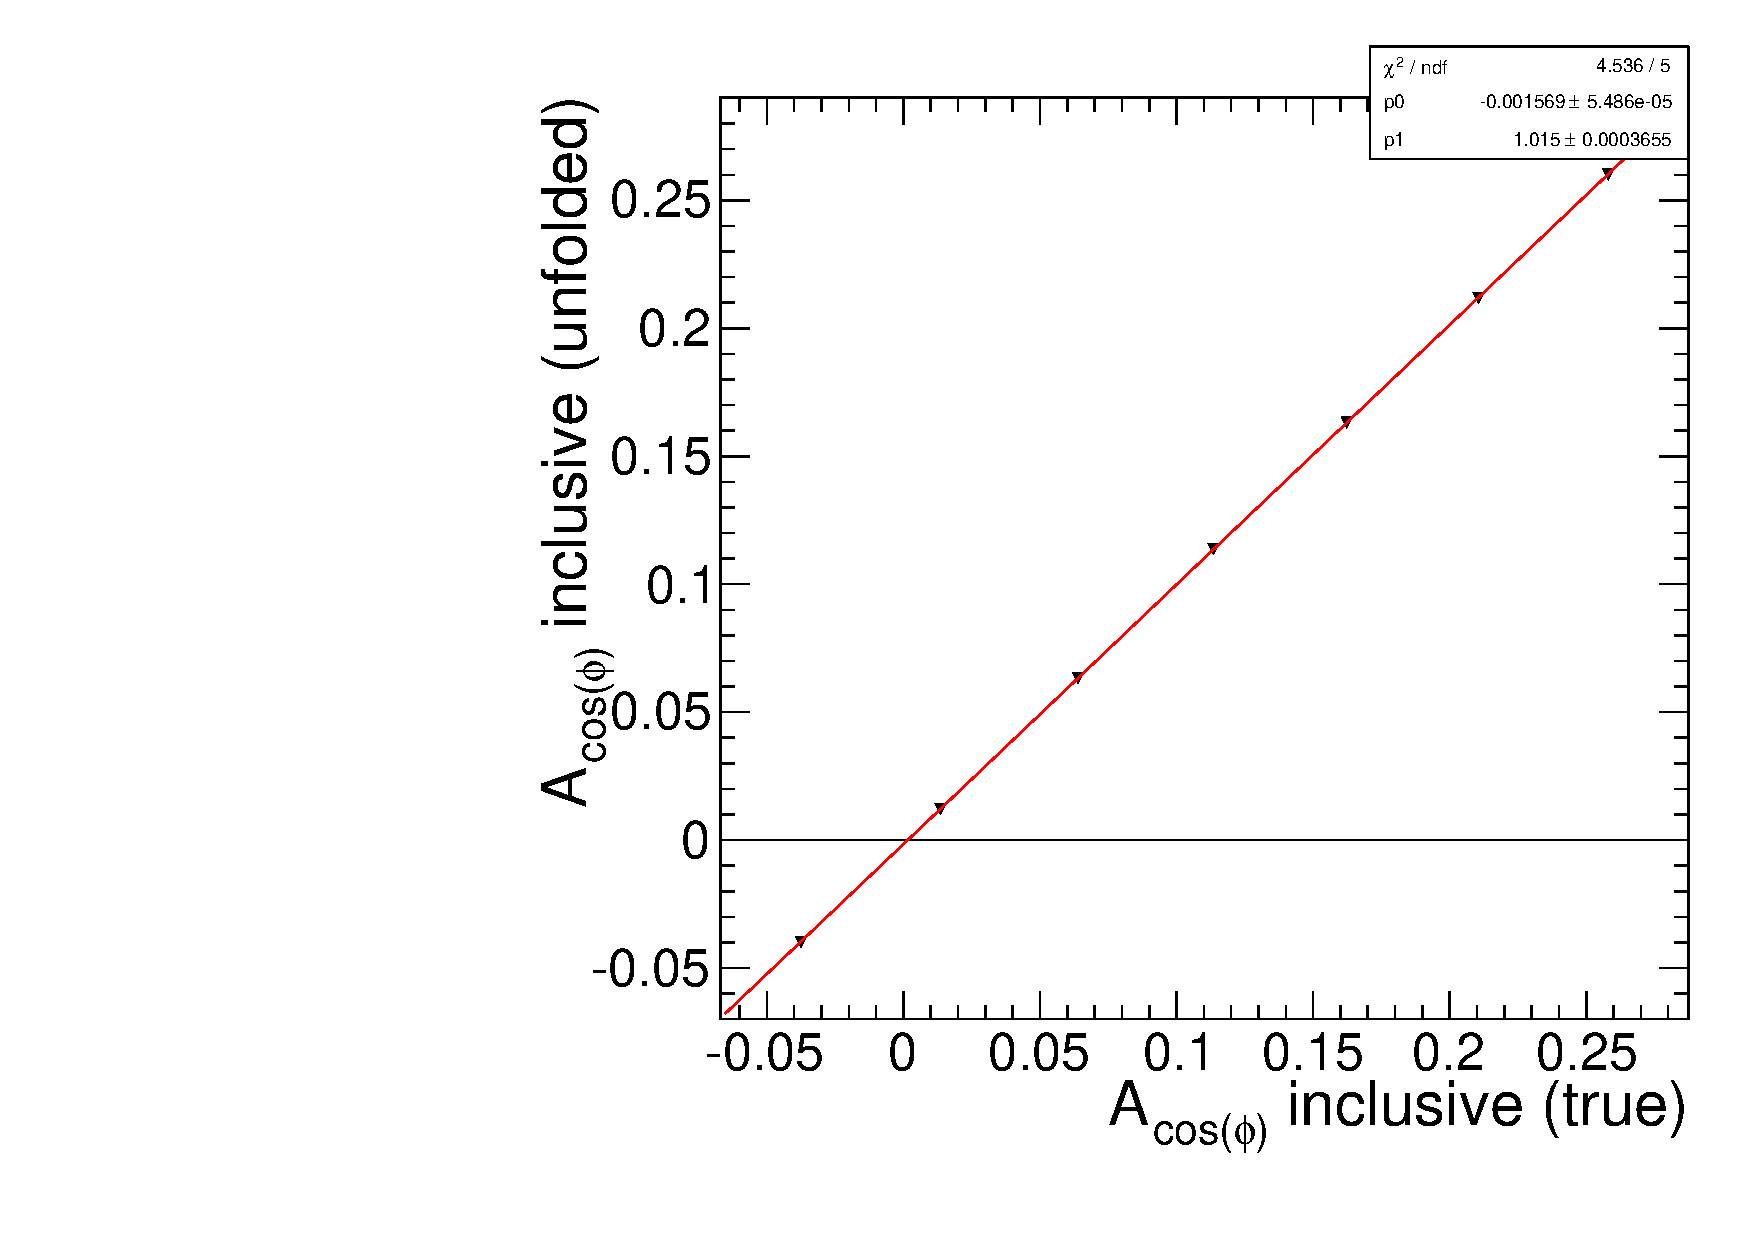
\includegraphics[width=0.325\linewidth]{figures/linearity_lepCosOpeningAngle.pdf}
\caption{Results of our linearity tests. Artificially induced
  asymmetry values are on the x-axis, and average unfolded asymmetries
  are on the y-axis.}
\label{fig:afb:linearity}
\end{figure}

% Table of linear fit parameters taken from AN-14-246. Unpublished.
\begin{table}[htpb]
\begin{center}
\caption{Parameters describing the fit to the linearity test results.}
\label{tab:afb:linearity}
\begin{tabular}{l |  c  c }
\hline
Variable &  offset  &  slope \\ \hline
$A^{lep}_{C}$       &   0.000 $\pm$ 0.000  &  1.000 $\pm$ 0.000\\ \hline
$A_{\Delta\phi}$ &   0.000 $\pm$ 0.000  &  1.002 $\pm$ 0.000\\ \hline
$A_{C}$          &   0.000 $\pm$ 0.000  &  1.001 $\pm$ 0.000\\ \hline
$A_{P}$          &   0.000 $\pm$ 0.000  &  1.023 $\pm$ 0.000\\ \hline
$A_{c1c2}$       &   0.002 $\pm$ 0.000  &  1.024 $\pm$ 0.000\\ \hline
$A_{\phi}$       &   -0.002 $\pm$ 0.000  &  1.015 $\pm$ 0.000\\ \hline
 \hline
\end{tabular}
\end{center}
\end{table}

In addition to the linearity tests, we also verify that the unfolding
uncertainties are estimated correctly by examining the \emph{pulls} of
the pseudoexperiments for each value of $K$. The pull is defined as:
\begin{equation}
\text{Pull} = \frac{A_{true} - A_{unfolded}}{\sigma(A_{unfolded})}
\end{equation}
When we plot these pulls for all observables and all values of $K$, we
find that they are gaussian distributed with a width of 1.0, meaning
that $\sigma(A_{unfolded})$ is estimated
correctly. Figure \ref{fig:afb:pulls} shows these pull
distributions for the example case of $K = 0$. Figure
\ref{fig:afb:pullwidths} shows the pull widths as a function of the
induced asymmetries.

% Pull distributions from AN-14-246. Unpublished.
\begin{figure}[htpb]
\centering
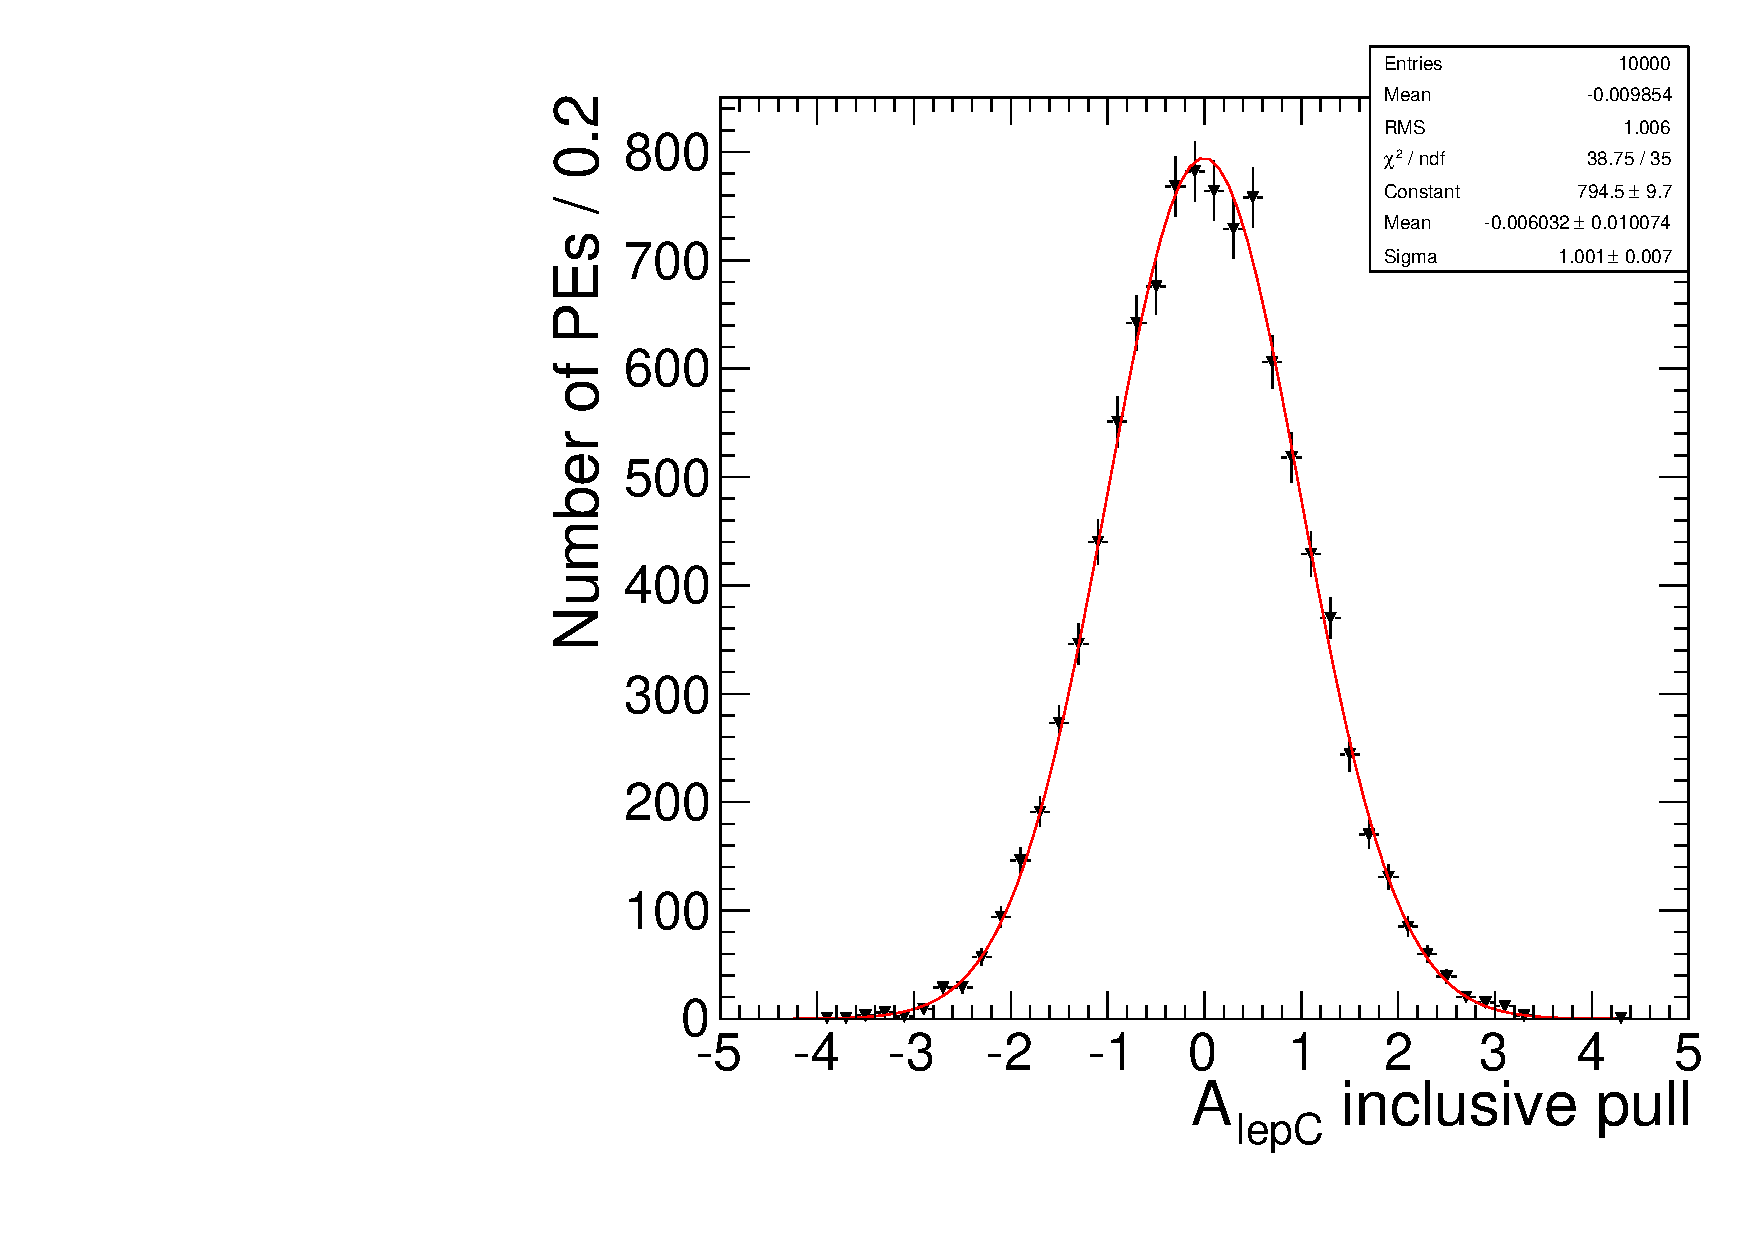
\includegraphics[width=0.325\linewidth]{figures/pull_lepChargeAsym.pdf}
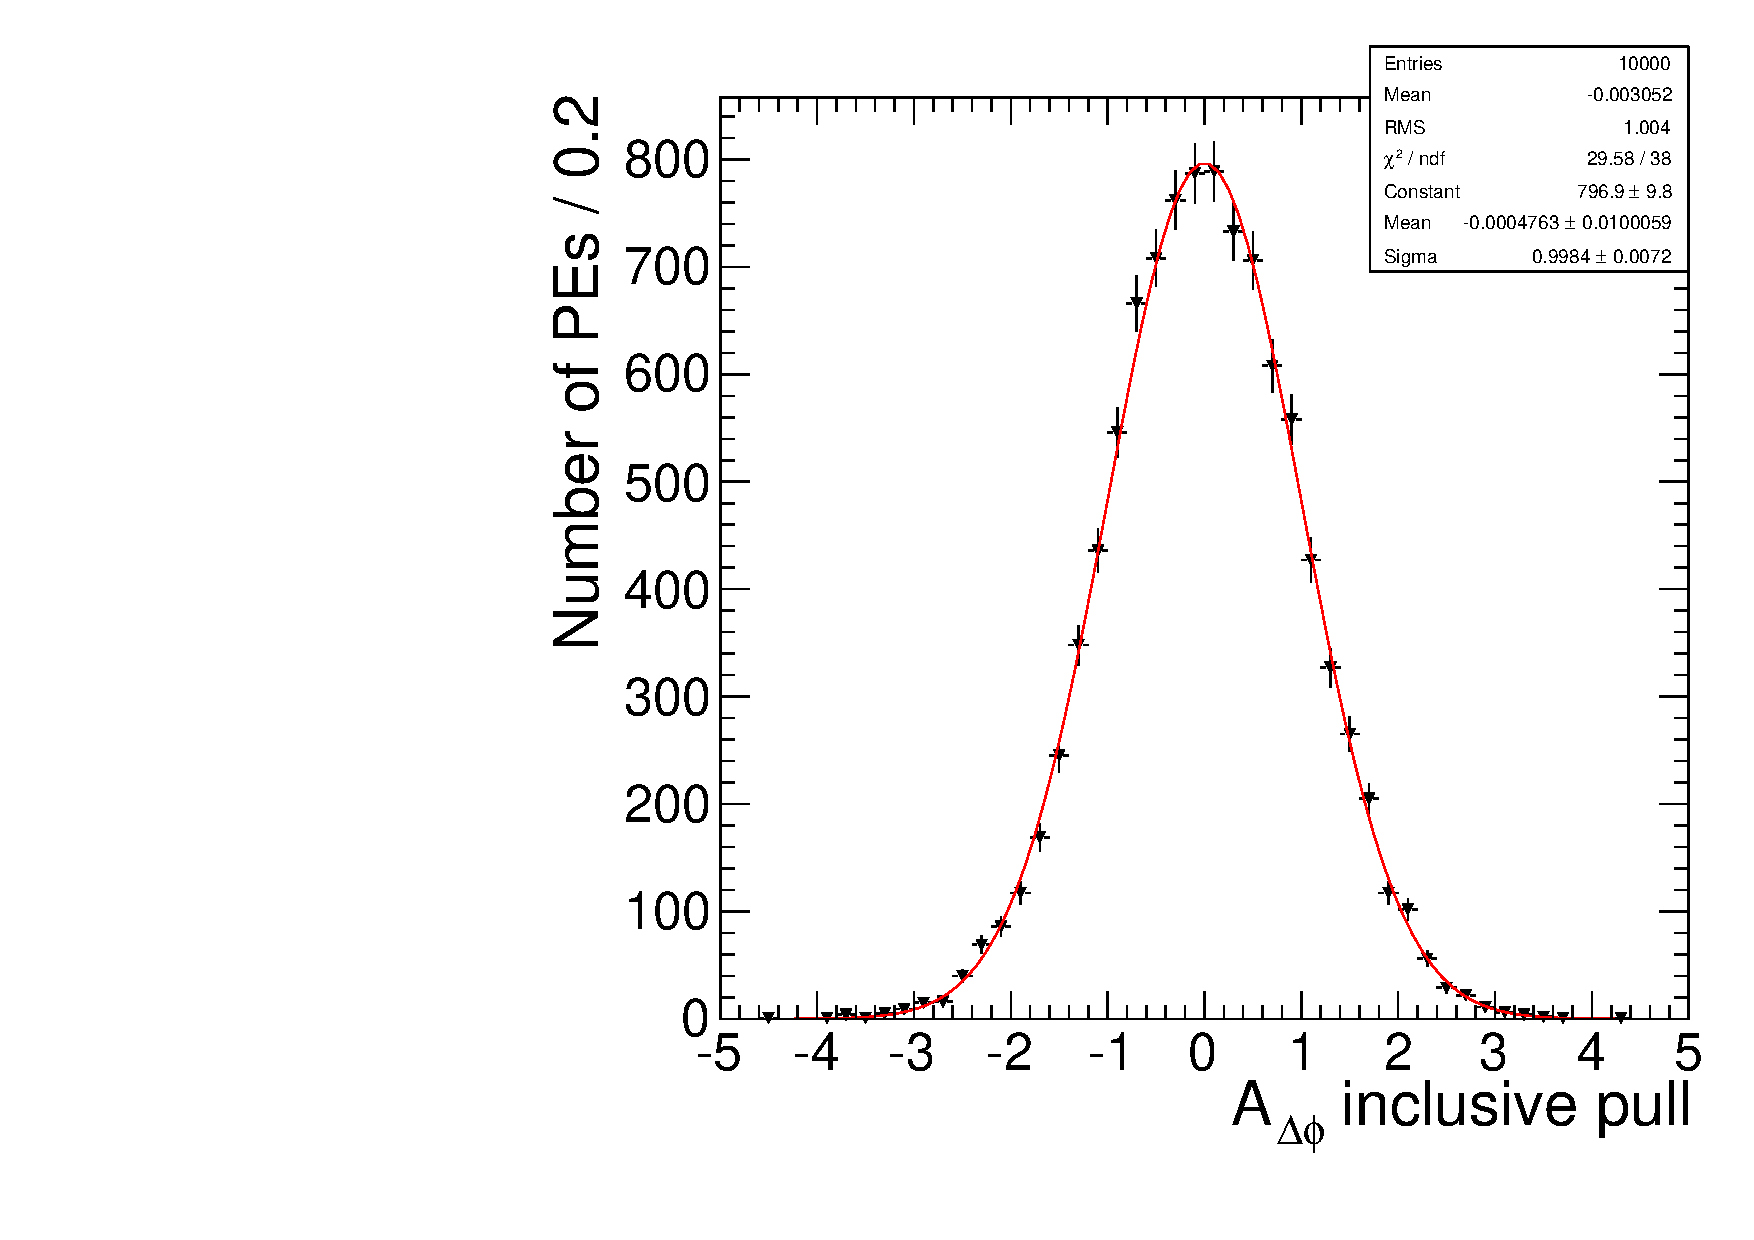
\includegraphics[width=0.325\linewidth]{figures/pull_lepAzimAsym2.pdf}
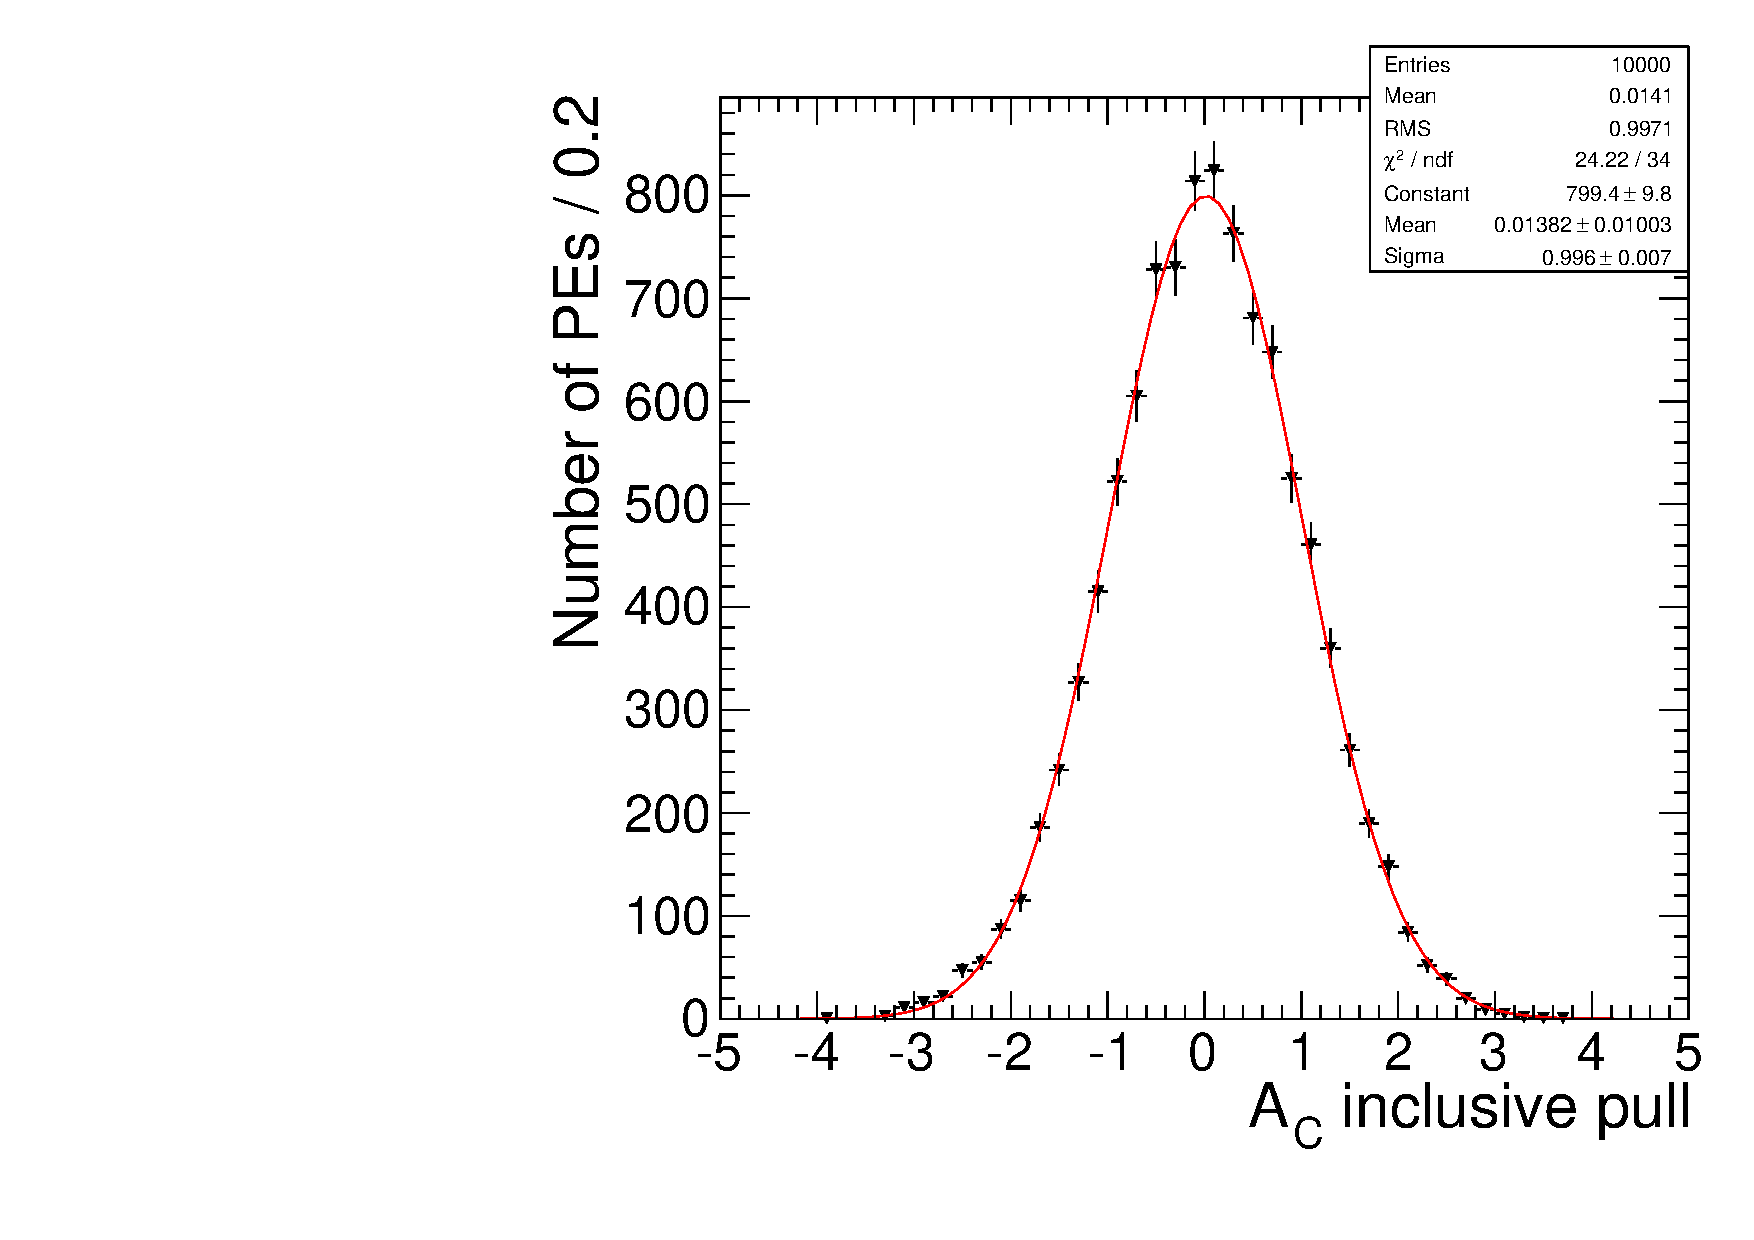
\includegraphics[width=0.325\linewidth]{figures/pull_rapiditydiffMarco.pdf}
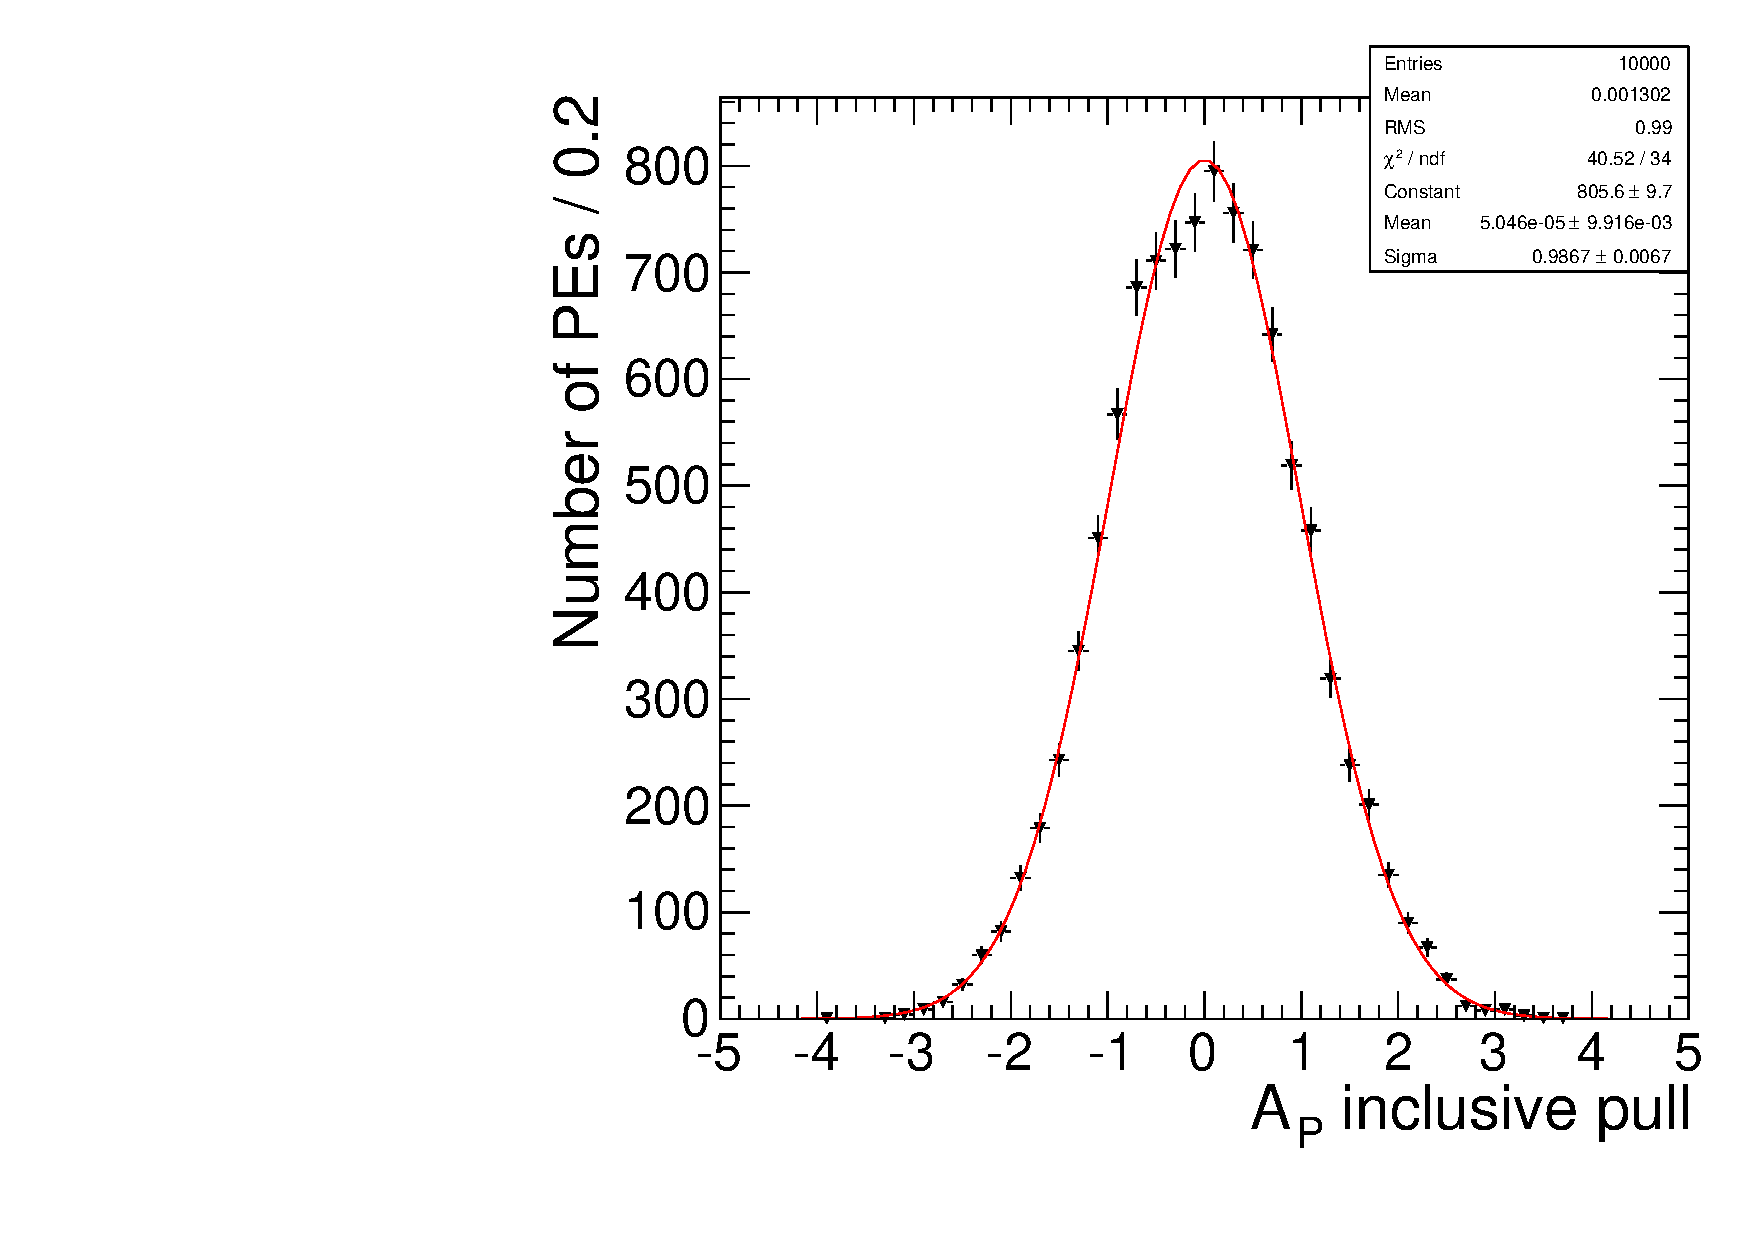
\includegraphics[width=0.325\linewidth]{figures/pull_lepCosTheta.pdf}
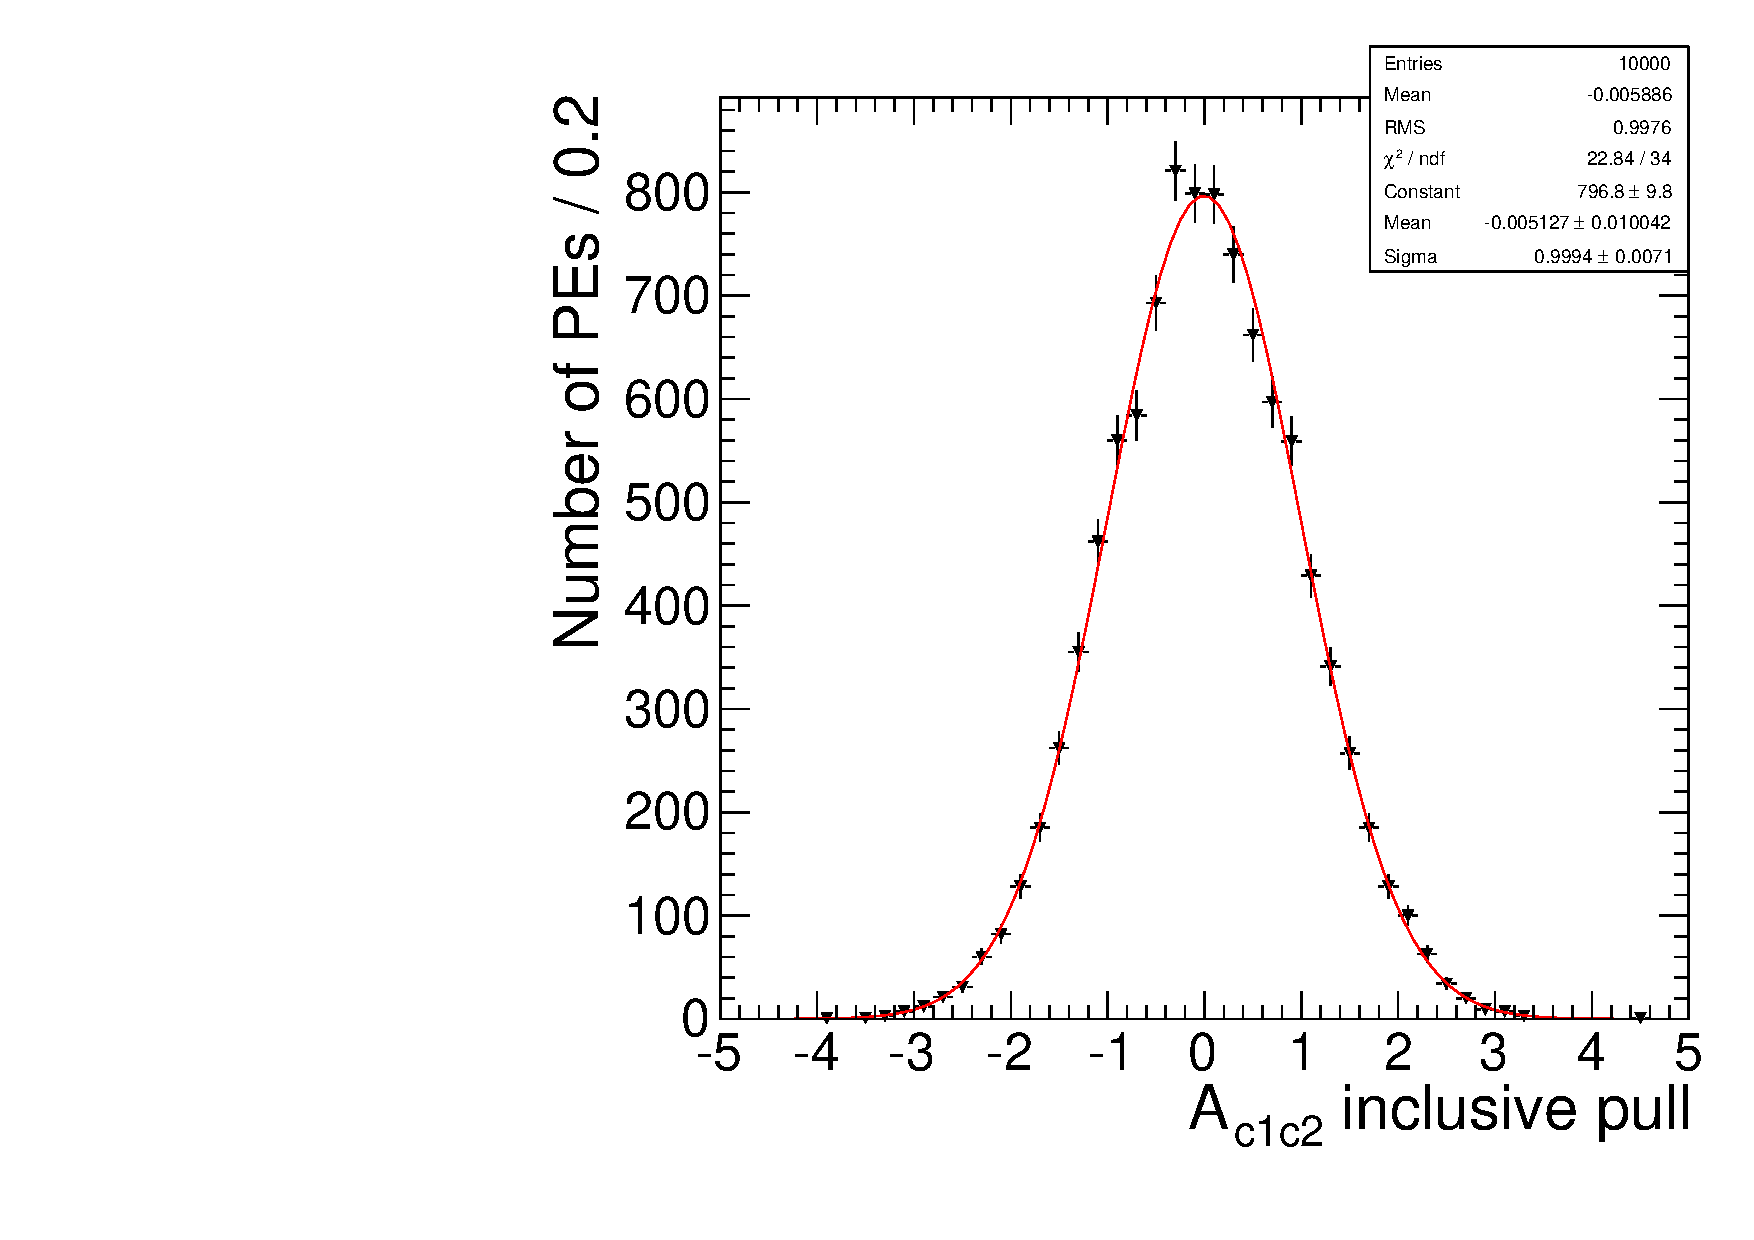
\includegraphics[width=0.325\linewidth]{figures/pull_topSpinCorr.pdf}
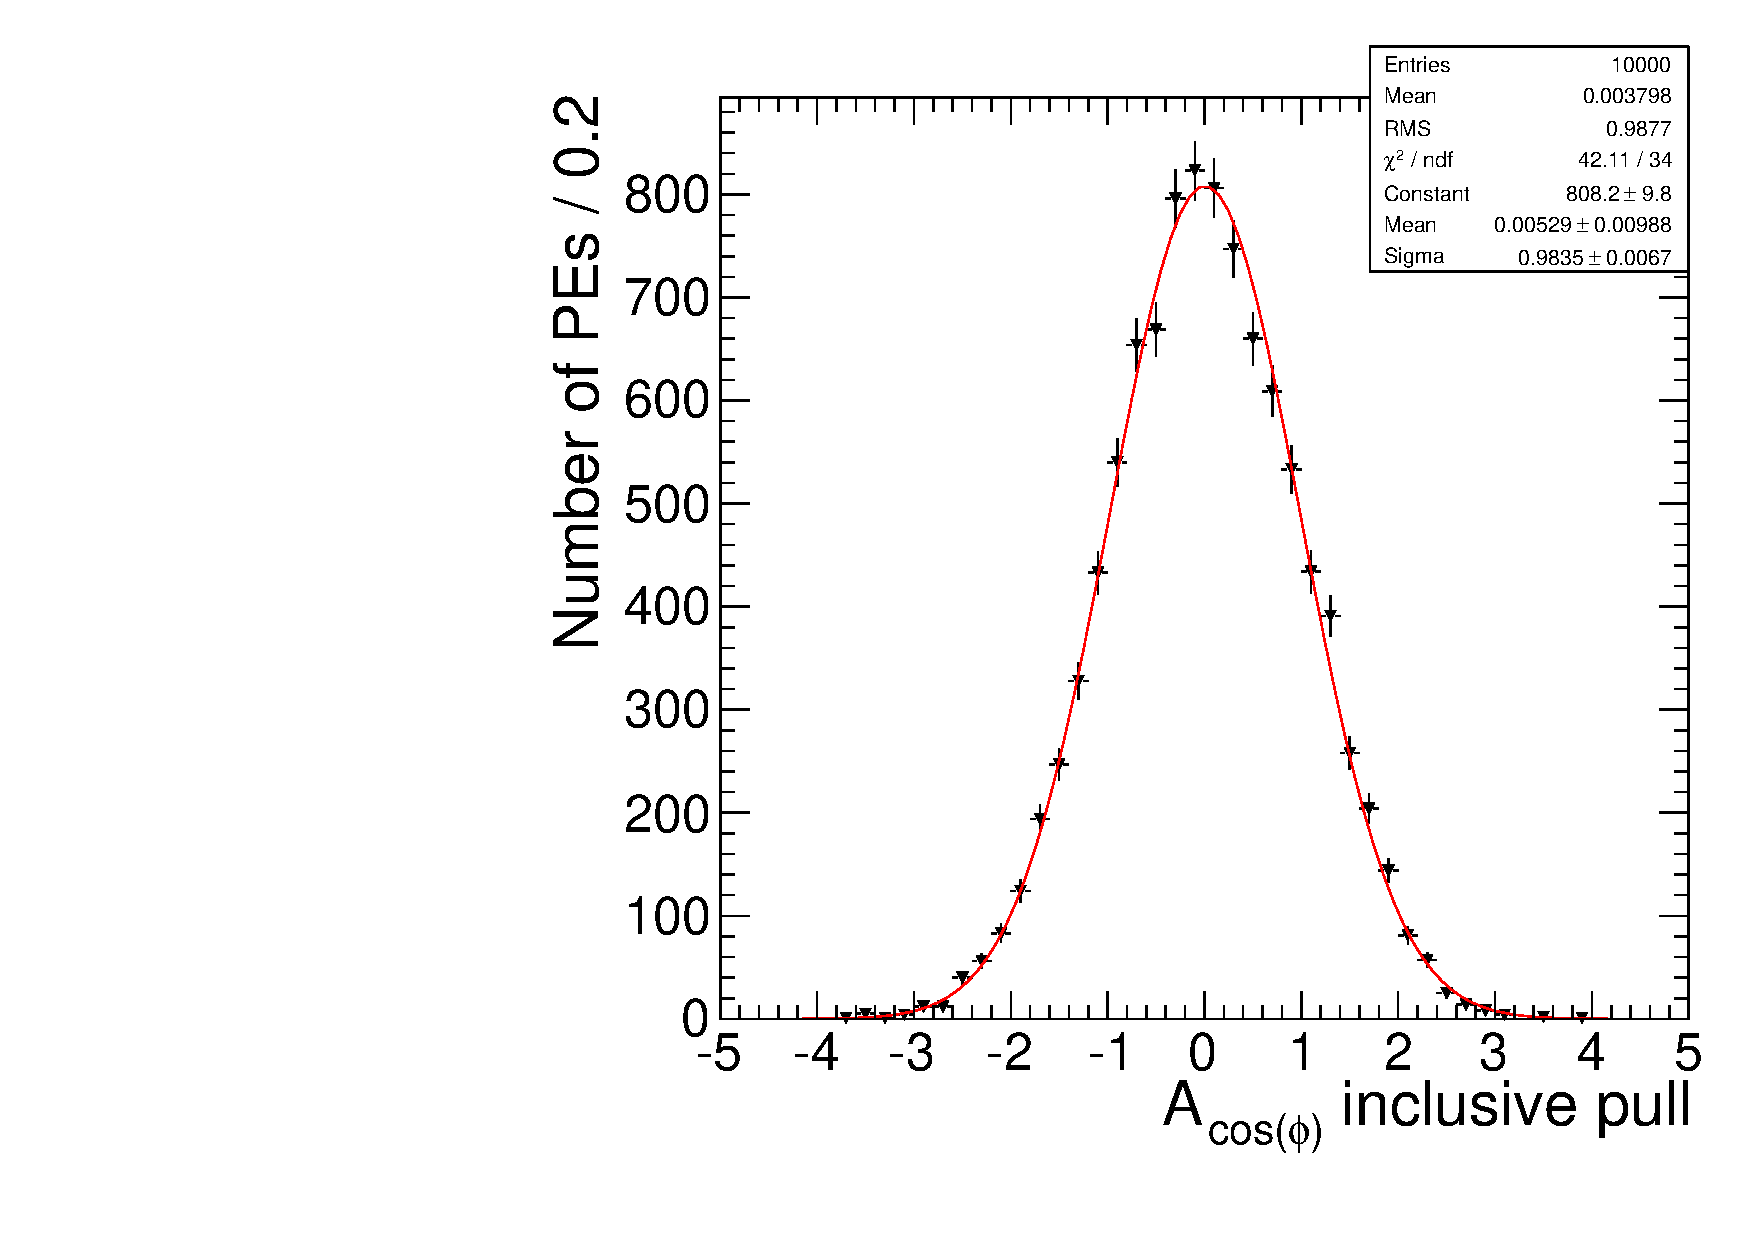
\includegraphics[width=0.325\linewidth]{figures/pull_lepCosOpeningAngle.pdf}
\caption{Pull distributions for the example case $K = 0$.}
\label{fig:afb:pulls}
\end{figure}

% Pull widths from AN-14-246. Unpublished.
\begin{figure}[htpb]
\centering
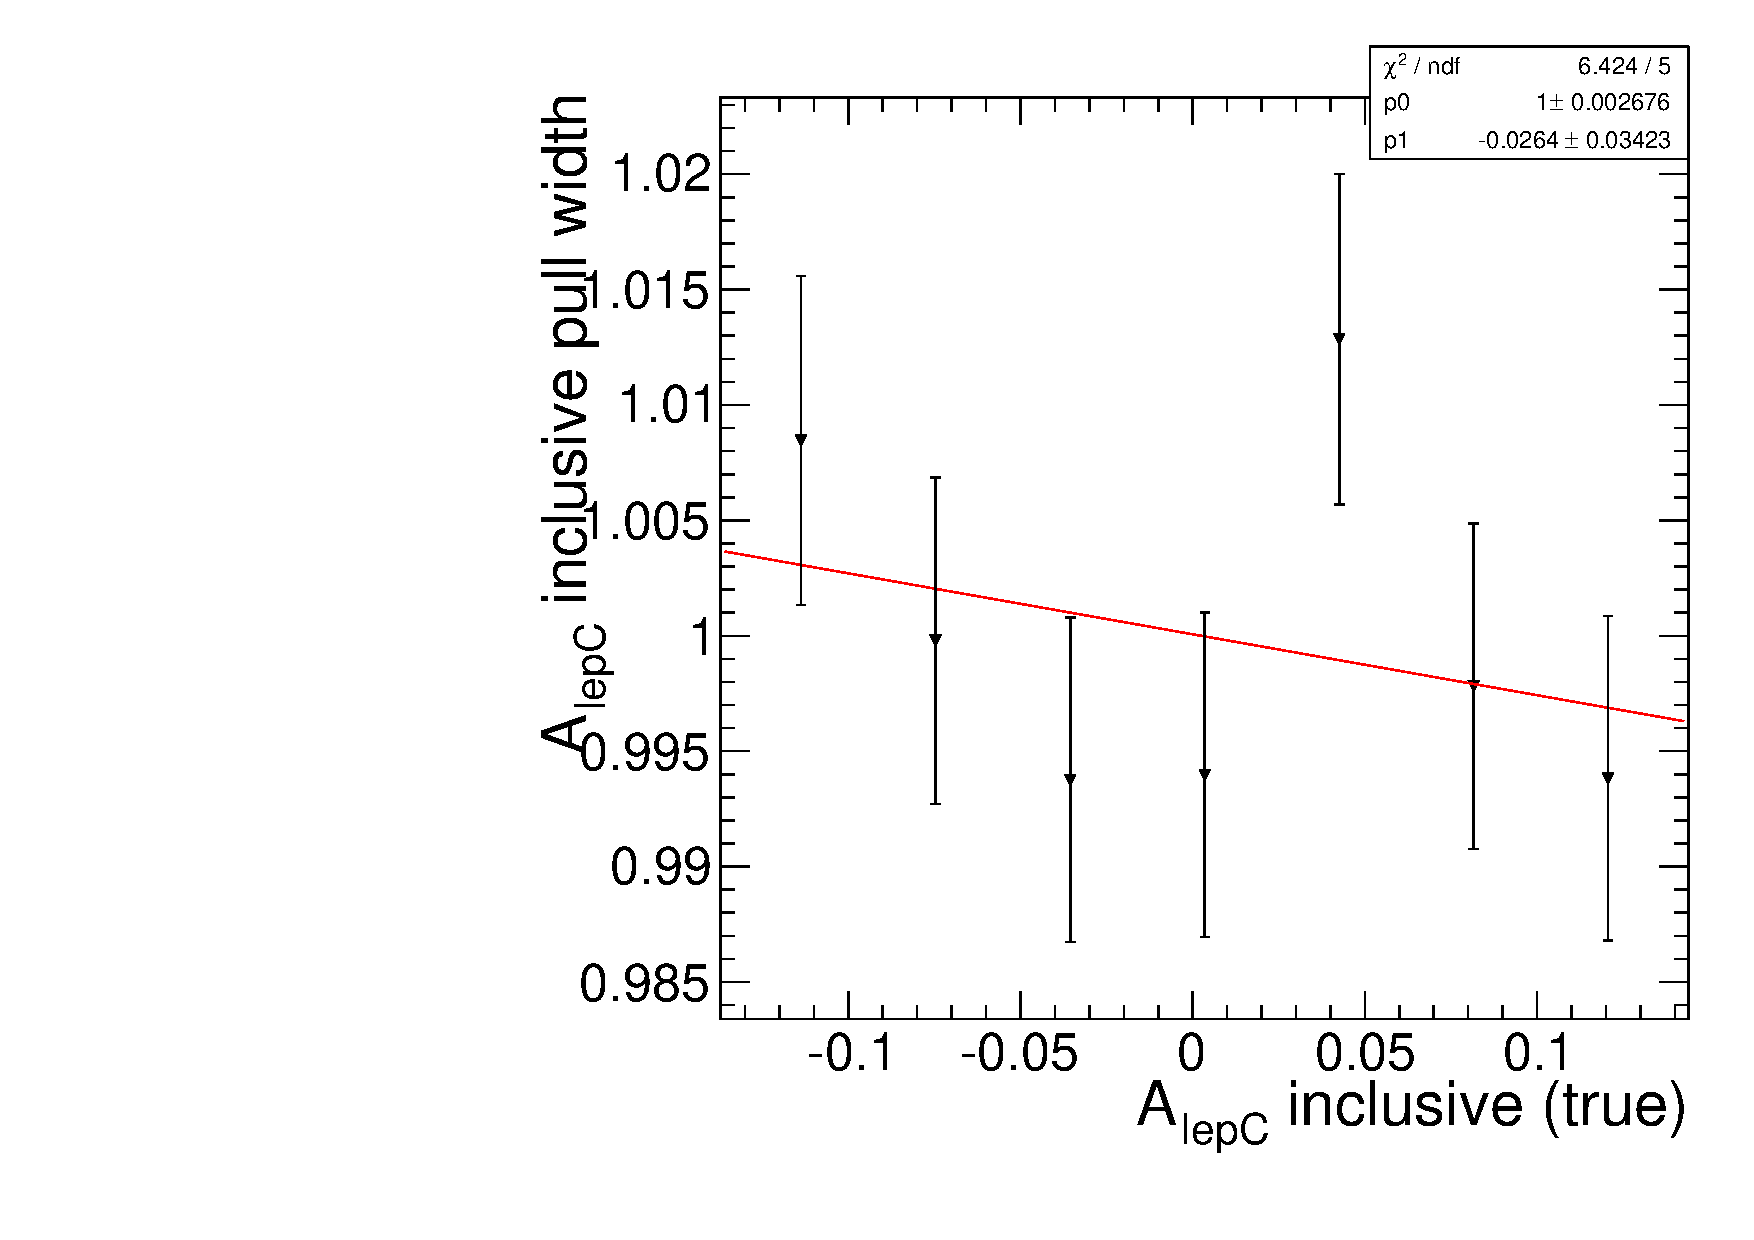
\includegraphics[width=0.325\linewidth]{figures/pullwidth_lepChargeAsym.pdf}
\includegraphics[width=0.325\linewidth]{figures/pullwidth_lepAzimAsym2.pdf}
\includegraphics[width=0.325\linewidth]{figures/pullwidth_rapiditydiffMarco.pdf}
\includegraphics[width=0.325\linewidth]{figures/pullwidth_lepCosTheta.pdf}
\includegraphics[width=0.325\linewidth]{figures/pullwidth_topSpinCorr.pdf}
\includegraphics[width=0.325\linewidth]{figures/pullwidth_lepCosOpeningAngle.pdf}
\caption{Pull widths for unfolded asymmetries vs. induced asymmetry
  values. Each data point corresponds to a single $K$ value. These
  results are consistent with pull widths of 1.}
\label{fig:afb:pullwidths}
\end{figure}

%%% Kick any other linearity and pull plots (e.g. for 2D unfolding) to an appendix.

\section{Systematic Uncertainties}
\label{sec:afb:systematics}

There are a number of possible mechanisms by which uncertainty may be
introduced into our asymmetry measurements. Most of these sources of
systematic uncertainty relate to imperfect modeling of the physics in our Monte
Carlo simulations, or to the workings of the CMS detector and
software. The ways in which we assign uncertainties
to these effects are discussed below. We will give special
consideration to the uncertainty due to regularization.

% Experimental systematics
Our experimental systematic uncertainties are evaluated as follows:

\begin{itemize}
\item \textbf{Lepton selection:} We correct the Monte Carlo
  simulations so that the lepton trigger efficiencies, and the
  efficiencies of lepton identification and isolation, reflect those
  measured in actual data. The scale factors used in these corrections
  never deviate from 1.0 by more than 2\%, so we vary all the scale
  factors by 2\% to obtain the lepton selection systematic.
\item \textbf{Lepton energy scale:} Comparisons between data and Monte
  Carlo for $Z \rightarrow \ell\ell$ events have shown that the
  uncertainty on electron energy scales is approximately 0.5\%; for
  muons, this uncertainty is negligible. Therefore we evaluate a
  systematic on the electron energy scale by varying that scale by
  0.5\%.
\item \textbf{Jet energy scale (JES):} The uncertainty from JES
  corrections is evaluated by varying those corrections within their
  uncertainties, and propagating the effect to the MET. We properly
  account for the effects this has on our event selections, and on the
  $\ttbar$ system reconstruction.
\item \textbf{Jet energy resolution (JER):} This uncertainty is
  evaluated similarly to the uncertainty on the JES. However, the JER
  is varied by 5-10\% depending on the $\eta$ of the jet.
\item \textbf{Background estimation:} We vary the normalizations of
  our backgrounds by the uncertainties evaluated in Section
  \ref{sec:afb:background}.
\item \textbf{Pileup (PU) modeling:} We vary the pileup reweighting
  scale factors by $\pm 1 \sigma$.
\item \textbf{b-tagging:} We reweight MC events to correctly model the
  efficiency of b-tagging $b$ and $c$ quarks. These scale factors are
  varied by $\pm 1 \sigma$.
\end{itemize}

% ttbar modeling systematics
In addition, there are several uncertainties on our modeling of the
$\ttdilep$ process. These uncertainties are evaluated as follows:

\begin{itemize}
\item \textbf{Factorization and renormalization scales:} We evaluate
  the uncertainty by substituting \textsc{mc@nlo} $\ttbar$ samples that have
  these two values scaled both up and down by a factor of 2.
\item \textbf{Top quark mass:} As described in Section
  \ref{ssec:afb:ttbarreconstruction}, we use 172.5 GeV for our top
  quark mass. To evaluate the systematic on this value, we use
  $\ttbar$ MC samples with the top mass varied by $\pm 3$ GeV, and
  interpolate down to an effective variation of $\pm 1$ GeV.
\item \textbf{Parton density functions (PDFs):} The systematic
  uncertainty on PDFs was evaluted using the then-current PDF4LHC
  recommendations \cite{pdf4lhc}.
\item \textbf{Top $p_T$ reweighting:} Since the effects of top $p_T$
  reweighting were not fully understood, we assigned a conservative
  100\% systematic to the reweighting.
\end{itemize}

Evaluating most of these systematics required us to regenerate the
smearing and acceptance matrices using reweighted Monte Carlo
simulations, and then reapply the unfolding procedure. In addition, we
evaluated the systematic uncertainty due to limited \textbf{Monte
  Carlo statistics} by propagating the uncertainty on the smearing
matrix to the unfolded result.

\subsubsection*{Regularization Systematic}

At the time this analysis was published, there was no standard way to
evaluate a systematic uncertainty on regularization. We therefore had
to devise our own method. We wished to isolate the effect of
regularization from other potential systematics related to the
unfolding. Specifically, we wished to separate regularization
uncertainty from any uncertainty that might arise if the MC used to
fill the smearing matrix is discrepant from real data. We argued that
any mismodeling in $S$ is already covered by the other systematic
uncertainties described above.

To evaluate the systematic uncertainty due to regularization, we
reweighted the bias distribution to match the data, and compared that
unfolded result to the nominal. This procedure should isolate the
effect of the regularization from any other sources of
uncertainty. As Section \ref{sec:afb:results} will show, the
uncertainty we obtain this way is less than 0.001 on
all asymmetry variables -- far smaller than the statistical
uncertainty on the results.

As a cross-check on the small size of this uncertainty, we
use pseudoexperiments to estimate the statistical uncertainty on our
choice of regularization strength, $\tau$. This check also gives an
uncertainty of $<0.001$ on all asymmetries. Further, this small
uncertainty is consistent with the findings from Section
\ref{ssec:afb:unfoldingtests}, that the bias induced by regularization
is a very small fraction of the total asymmetry.

To validate the claim that any mismodeling of the smearing matrix is
covered by other systematics, we tried reweighting both the bias
distribution and $S$ together. The uncertainty produced by this test
was still smaller in magnitude than the sum of the other systematics,
so we can be confident that those systematics cover any mismodeling in
$S$.

Finally, we verified that the regularization term contributes only a
small amount to the $\chi^2$ that is minimized in the unfolding
procedure.
% There's a table of chi^2 values, but do I really need it here?
% Probably not, since I don't give hard numbers for the tau variation
% either.

The systematic uncertainties on our asymmetry measurements are
summarized in Table \ref{tab:afb:systematics}.

% Systematics table pulled from AN-14-246.
\begin{table}[!h]
\begin{center}
\caption{Systematic uncertainties on the inclusive unfolded asymmetry measurements.}
\label{tab:afb:systematics}
\begin{tabular}{l||r|r|r|r|r|r}
\hline
Asymmetry variable              &       \multicolumn{1}{c|}{$A_{C}$}            &       \multicolumn{1}{c|}{$A^{lep}_{C}$}
        &       \multicolumn{1}{c|}{$A_{\Delta\phi}$}           &       \multicolumn{1}{c|}{$A_{\cos\phi}$}  &       \multicolumn{1}{c|}{$A_{c1c2}$}  &       \multicolumn{1}{c|}{$A_{P}$}  \\
\hline
\hline
\multicolumn{6}{c}{experimental systematic uncertainties} \\
\hline
Jet energy scale                  & $0.001$   & $0.000$   & $0.001$   & $0.005$   & $0.007$   & $0.018$   \\
Jet energy resolution             & $0.002$   & $0.000$   & $0.000$   & $0.001$   & $0.002$   & $0.003$   \\
Lepton energy scale               & $0.001$   & $0.000$   & $0.001$   & $0.002$   & $0.005$   & $0.003$   \\
b-tagging efficiency              & $0.001$   & $0.000$   & $0.000$   & $0.001$   & $0.001$   & $0.001$   \\
Lepton selection                  & $0.000$   & $0.000$   & $0.001$   & $0.000$   & $0.000$   & $0.002$   \\
Pileup                            & $0.000$   & $0.000$   & $0.000$   & $0.000$   & $0.000$   & $0.000$   \\
Background                        & $0.001$   & $0.001$   & $0.001$   & $0.001$   & $0.001$   & $0.002$   \\
\hline
\hline
\multicolumn{6}{c}{$\ttbar$ modeling uncertainties} \\
\hline
Top quark mass                    & $0.001$   & $0.001$   & $0.001$   & $0.001$   & $0.007$   & $0.008$   \\
Fact. and renorm. scales          & $0.003$   & $0.002$   & $0.002$   & $0.003$   & $0.005$   & $0.002$   \\
Parton distribution functions     & $0.001$   & $0.001$   & $0.004$   & $0.005$   & $0.005$   & $0.001$   \\
Hadronization                     & $0.003$   & $0.000$   & $0.001$   & $0.004$   & $0.005$   & $0.019$   \\
\hline
\hline
Unfolding (simulation statistics) & $0.005$   & $0.002$   & $0.002$   & $0.005$   & $0.006$   & $0.003$   \\
Unfolding (regularization)        & $0.000$   & $0.000$   & $0.000$   & $0.000$   & $0.000$   & $0.000$   \\
\hline
\hline
Top quark $p_T$                   & $0.001$   & $0.000$   & $0.011$   & $0.006$   & $0.006$   & $0.004$   \\
\hline
\hline
Total systematic uncertainty      & $0.007$   & $0.003$   & $0.012$   & $0.012$   & $0.016$   & $0.028$   \\
\hline
\hline
Total uncertainty (inc. data stat.) & $0.013$   & $0.006$   & $0.013$   & $0.016$   & $0.021$   & $0.029$   \\
\hline
\end{tabular}
\end{center}
\end{table}

\section{Results and Interpretation}
\label{sec:afb:results}

\subsection{One-Dimensional Results}
\label{ssec:afb:results1d}

After subtracting the background and unfolding, distributions for our
six asymmetry variables are shown in Figure \ref{fig:afb:results1d},
along with SM parton-level predictions using
\textsc{mc@nlo} and NLO+EW predictions. The
measured asymmetry values with uncertainties and the \textsc{mc@nlo}
predictions are presented numerically in Table
\ref{tab:afb:results1d}. All six asymmetries are consistent with the
predictions; thus, we do not observe any significant deviations from
the Standard Model expectation.

% Plots taken from AN-14-246. Charge asymmetry plots are a wee bit
% different from published versions, which say "NLO (QCD+EW)", and
% have horizontal error bars on the ratio plot markers
\begin{figure}[hbtp]
\centering
\includegraphics[width=0.325\linewidth]{figures/results_1D_rapiditydiffMarco.pdf}
\includegraphics[width=0.325\linewidth]{figures/results_1D_lepChargeAsym.pdf}
\includegraphics[width=0.325\linewidth]{figures/results_1D_lepAzimAsym2.pdf}
\includegraphics[width=0.325\linewidth]{figures/results_1D_lepCosTheta.pdf}
\includegraphics[width=0.325\linewidth]{figures/results_1D_topSpinCorr.pdf}
\includegraphics[width=0.325\linewidth]{figures/results_1D_lepCosOpeningAngle.pdf}
\caption{Distributions of asymmetry variables after
  unfolding, and simulations and theoretical predictions.}
\label{fig:afb:results1d}
\end{figure}

% Results table taken from AN-14-246
\begin{table}[hbtp]
\begin{center}
\caption{Asymmetry values measured after unfolding, compared to
  predictions from simulation. Uncertainties on measurements are
  statistical and systematic; uncertainties on simulation are
  statistical only.}
\label{tab:afb:results1d}
\begin{tabular}{l |  c  c }
\hline
Variable &  Data  &  MC \\ \hline
$A_{C}$ & $0.011 \pm 0.011 \pm 0.007$  &  $ 0.006 \pm 0.001$  \\
$A^{lep}_{C}$ & $0.003 \pm 0.006 \pm 0.003$  &  $ 0.004 \pm 0.001$   \\
$A_{\Delta\phi}$ & $0.094 \pm 0.005 \pm 0.012$  &  $ 0.113 \pm 0.001$   \\
$A_{\cos\phi}$ & $0.102 \pm 0.010 \pm 0.012$  &  $ 0.114 \pm 0.001$ \\
$A_{c1c2}$ & $-0.069 \pm 0.013 \pm 0.016$  &  $ -0.081 \pm 0.001$  \\
$A_{P}$ & $-0.011 \pm 0.007 \pm 0.028$  &  $ 0.000 \pm 0.001$       \\
% $A_{P}^{\rm{CPV}}$ & $-0.000 \pm 0.006 \pm 0.005$  &  $ 0$         \\
 \hline
\end{tabular}
\end{center}
\end{table}

\subsection{Two-Dimensional Results}
\label{ssec:afb:results2d}

After 2D unfolding, the six asymmetries, along with \textsc{mc@nlo}
and NLO+EW predictions, are presented differentially
with respect to $m_{\ttbar}$, $|y_{\ttbar}|$, and $p_T^{\ttbar}$ in
Figures \ref{fig:afb:results2d:chargeasym} and
\ref{fig:afb:results2d:spincorrpol}. The overall values of these
2D-unfolded asymmetries, and the corresponding MC predictions, are presented in
Table \ref{tab:afb:results2d:inclusive}. The asymmetry values for each
bin in the secondary variables are presented in Table
\ref{tab:afb:results2d:binbybin}. The overall 2D-unfolded asymmetries
are consistent with the MC predictions; therefore, we do not observe
any discrepancy from the Standard Model expectation.

% Charge asym figures taken from AN-14-246. Slightly different from
% published plots, which say "NLO (QCD+EW)" instead of "NLO+EW".
\begin{figure}[!hbtp]
\centering
\includegraphics[width=0.325\linewidth]{figures/results_2D_rapiditydiffMarco_vsmtt.pdf}
\includegraphics[width=0.325\linewidth]{figures/results_2D_rapiditydiffMarco_vsttrapidity2.pdf}
\includegraphics[width=0.325\linewidth]{figures/results_2D_rapiditydiffMarco_vsttpt.pdf}
\includegraphics[width=0.325\linewidth]{figures/results_2D_lepChargeAsym_vsmtt.pdf}
\includegraphics[width=0.325\linewidth]{figures/results_2D_lepChargeAsym_vsttrapidity2.pdf}
\includegraphics[width=0.325\linewidth]{figures/results_2D_lepChargeAsym_vsttpt.pdf}
\caption{Unfolded charge asymmetry values as a function of the three
  secondary kinematic variables. The last bin includes any overflow.}
\label{fig:afb:results2d:chargeasym}
\end{figure}

% Spin corr and pol figures taken from AN-14-246. Published.
\begin{figure}[!hbtp]
\centering
\includegraphics[width=0.325\linewidth]{figures/results_2D_lepAzimAsym2_vsmtt.pdf}
\includegraphics[width=0.325\linewidth]{figures/results_2D_lepAzimAsym2_vsttrapidity2.pdf}
\includegraphics[width=0.325\linewidth]{figures/results_2D_lepAzimAsym2_vsttpt.pdf}
\includegraphics[width=0.325\linewidth]{figures/results_2D_lepCosTheta_vsmtt.pdf}
\includegraphics[width=0.325\linewidth]{figures/results_2D_lepCosTheta_vsttrapidity2.pdf}
\includegraphics[width=0.325\linewidth]{figures/results_2D_lepCosTheta_vsttpt.pdf}
\includegraphics[width=0.325\linewidth]{figures/results_2D_topSpinCorr_vsmtt.pdf}
\includegraphics[width=0.325\linewidth]{figures/results_2D_topSpinCorr_vsttrapidity2.pdf}
\includegraphics[width=0.325\linewidth]{figures/results_2D_topSpinCorr_vsttpt.pdf}
\includegraphics[width=0.325\linewidth]{figures/results_2D_lepCosOpeningAngle_vsmtt.pdf}
\includegraphics[width=0.325\linewidth]{figures/results_2D_lepCosOpeningAngle_vsttrapidity2.pdf}
\includegraphics[width=0.325\linewidth]{figures/results_2D_lepCosOpeningAngle_vsttpt.pdf}
\caption{Unfolded spin correlation and polarization asymmetry values
  as a function of the three secondary kinematic variables. The last
  bin includes any overflow.}
\label{fig:afb:results2d:spincorrpol}
\end{figure}

% Inclusive 2D asymmetries adapted from AN-14-246. Not published, but
% can be inferred from published plots.
\begin{table}[hbt]
\begin{center}
\caption{Measured asymmetries after 2D unfolding, for each of the
  secondary kinematic variables. Uncertainties on measured asymmetries
  are statistical and systematic; uncertainties on simulation are
  statistical only.}
\label{tab:afb:results2d:inclusive}
\begin{tabular}{l |  c  c }
\hline
Variable &  Unfolded vs $M_{\ttbar}$  &  MC \\ \hline
$A_{C}$                                 & 0.009 $\pm$ 0.013     $\pm$ 0.008      & 0.006 $\pm$  0.001 \\
$A^{lep}_{C}$                              & -0.002 $\pm$ 0.006 $\pm$ 0.003         & 0.004 $\pm$  0.001 \\
$A_{\Delta\phi}$        & 0.095 $\pm$ 0.006     $\pm$ 0.007          & 0.113 $\pm$  0.001 \\
$A_{c1c2}$                              & -0.065 $\pm$ 0.015 $\pm$ 0.015         & -0.081 $\pm$  0.001 \\
$A_{P}$                   & -0.011 $\pm$ 0.008 $\pm$ 0.028         & 0.000 $\pm$  0.001 \\
$A_{\cos\phi}$                              & 0.094 $\pm$ 0.012 $\pm$ 0.009      & 0.114 $\pm$  0.001 \\
% $A_{P}$ (CP+)                   & -0.011 $\pm$ 0.008 $\pm$ 0.028         & 0.000 $\pm$  0.001 \\
% $A_{P}$ (CP-)                   & -0.001 $\pm$ 0.007 $\pm$ 0.006         & 0 \\
 \hline

\hline
Variable &  Unfolded vs $y_{\ttbar}$  &  MC \\ \hline
$A_{C}$                                 & 0.016 $\pm$ 0.012     $\pm$ 0.007      & 0.006 $\pm$  0.001 \\
$A^{lep}_{C}$                              & 0.002 $\pm$ 0.006     $\pm$ 0.003          & 0.004 $\pm$  0.001 \\
$A_{\Delta\phi}$        & 0.095 $\pm$ 0.006     $\pm$ 0.012          & 0.113 $\pm$  0.001 \\
$A_{c1c2}$                              & -0.077 $\pm$ 0.015 $\pm$ 0.019         & -0.081 $\pm$  0.001 \\
$A_{P}$                   & -0.010 $\pm$ 0.008 $\pm$ 0.029         & 0.000 $\pm$  0.001 \\
$A_{\cos\phi}$                              & 0.097 $\pm$ 0.011     $\pm$ 0.012      & 0.114 $\pm$  0.001 \\
% $A_{P}$ (CP+)                   & -0.010 $\pm$ 0.008 $\pm$ 0.030         & 0.000 $\pm$  0.001 \\
% $A_{P}$ (CP-)                   & -0.002 $\pm$ 0.007 $\pm$ 0.007         & 0 \\
 \hline

\hline
Variable &  Unfolded vs $p_T^{\ttbar}$  &  MC \\ \hline
$A_{C}$                                 & 0.011 $\pm$ 0.012     $\pm$ 0.008      & 0.006 $\pm$  0.001 \\
$A^{lep}_{C}$                              & 0.001 $\pm$ 0.006     $\pm$ 0.003          & 0.004 $\pm$  0.001 \\
$A_{\Delta\phi}$                & 0.094 $\pm$ 0.006     $\pm$ 0.012          & 0.113 $\pm$  0.001 \\
$A_{c1c2}$                              & -0.072 $\pm$ 0.014 $\pm$ 0.017         & -0.081 $\pm$  0.001 \\
$A_{P}$                   & -0.014 $\pm$ 0.008 $\pm$ 0.028         & 0.000 $\pm$  0.001 \\
$A_{\cos\phi}$                              & 0.100 $\pm$ 0.011     $\pm$ 0.011          & 0.114 $\pm$  0.001 \\
% $A_{P}$ (CP+)                   & -0.014 $\pm$ 0.008 $\pm$ 0.028         & 0.000 $\pm$  0.001 \\
% $A_{P}$ (CP-)                   & 0.001 $\pm$ 0.007 $\pm$ 0.006          & 0 \\
 \hline
\end{tabular}
\end{center}
\end{table}

% Bin-by-bin 2D asymmetries adapted from AN-14-246. Not published, but
% can be inferred from published plots.
\begin{table}[hbt]
\begin{center}
\caption{Measured asymmetry values after 2D unfolding, presented
  bin-by-bin in the secondary kinematic variables. Uncertainties on
  measured values are statistical and systematic.}
\label{tab:afb:results2d:binbybin}
\begin{tabular}{l |  c  c  c }
\hline
Variable & $M_{\ttbar}$ bin 1 & $M_{\ttbar}$ bin 2 & $M_{\ttbar}$ bin 3  \\ \hline
$A_{C}$  & $0.007 \pm 0.031 \pm 0.019$   & $0.015 \pm 0.029 \pm 0.015$   & $0.004 \pm 0.021 \pm 0.013$  \\
$A^{lep}_{C}$  & $-0.023 \pm 0.014 \pm 0.009$   & $0.010 \pm 0.016 \pm 0.009$   & $0.015 \pm 0.016 \pm 0.010$  \\
$A_{\Delta\phi}$  & $-0.048 \pm 0.014 \pm 0.012$   & $0.108 \pm 0.016 \pm 0.014$   & $0.283 \pm 0.017 \pm 0.026$  \\
$A_{\cos\phi}$  & $0.111 \pm 0.024 \pm 0.024$   & $0.103 \pm 0.031 \pm 0.022$   & $0.059 \pm 0.026 \pm 0.021$  \\
$A_{c1c2}$  & $-0.053 \pm 0.032 \pm 0.031$   & $-0.090 \pm 0.029 \pm 0.032$   & $-0.056 \pm 0.026 \pm 0.030$  \\
$A_{P}$  & $-0.017 \pm 0.020 \pm 0.025$   & $-0.013 \pm 0.019 \pm 0.038$   & $0.000 \pm 0.017 \pm 0.035$  \\
%$A_{P}^{\rm{CPV}}$  & $-0.029 \pm 0.016 \pm 0.013$   & $0.049 \pm 0.017 \pm 0.013$   & $-0.018 \pm 0.012 \pm 0.016$  \\
 \hline

\hline
Variable & $y_{\ttbar}$ bin 1 & $y_{\ttbar}$ bin 2 & $y_{\ttbar}$ bin 3  \\ \hline
$A_{C}$  & $-0.002 \pm 0.031 \pm 0.013$   & $0.016 \pm 0.027 \pm 0.017$   & $0.029 \pm 0.022 \pm 0.014$  \\
$A^{lep}_{C}$  & $-0.001 \pm 0.015 \pm 0.009$   & $-0.024 \pm 0.015 \pm 0.010$   & $0.023 \pm 0.013 \pm 0.006$  \\
$A_{\Delta\phi}$  & $0.103 \pm 0.014 \pm 0.012$   & $0.092 \pm 0.016 \pm 0.015$   & $0.090 \pm 0.013 \pm 0.015$  \\
$A_{\cos\phi}$  & $0.115 \pm 0.023 \pm 0.021$   & $0.115 \pm 0.024 \pm 0.019$   & $0.070 \pm 0.021 \pm 0.022$  \\
$A_{c1c2}$  & $-0.063 \pm 0.028 \pm 0.027$   & $-0.073 \pm 0.028 \pm 0.023$   & $-0.089 \pm 0.027 \pm 0.029$  \\
$A_{P}$  & $-0.018 \pm 0.017 \pm 0.034$   & $-0.012 \pm 0.018 \pm 0.029$   & $-0.003 \pm 0.016 \pm 0.031$  \\
%$A_{P}^{\rm{CPV}}$  & $0.006 \pm 0.021 \pm 0.016$   & $0.011 \pm 0.015 \pm 0.017$   & $-0.016 \pm 0.011 \pm 0.010$  \\
 \hline

\hline
Variable & $p_T^{\ttbar}$ bin 1 & $p_T^{\ttbar}$ bin 2 & $p_T^{\ttbar}$ bin 3  \\ \hline
$A_{C}$  & $0.009 \pm 0.018 \pm 0.012$   & $-0.033 \pm 0.033 \pm 0.027$   & $0.084 \pm 0.036 \pm 0.026$  \\
$A^{lep}_{C}$  & $0.006 \pm 0.010 \pm 0.005$   & $-0.020 \pm 0.016 \pm 0.015$   & $0.015 \pm 0.018 \pm 0.010$  \\
$A_{\Delta\phi}$  & $0.101 \pm 0.010 \pm 0.016$   & $0.108 \pm 0.016 \pm 0.017$   & $0.049 \pm 0.018 \pm 0.020$  \\
$A_{\cos\phi}$  & $0.081 \pm 0.017 \pm 0.017$   & $0.149 \pm 0.031 \pm 0.020$   & $0.084 \pm 0.035 \pm 0.037$  \\
$A_{c1c2}$  & $-0.073 \pm 0.020 \pm 0.019$   & $-0.060 \pm 0.038 \pm 0.039$   & $-0.086 \pm 0.043 \pm 0.038$  \\
$A_{P}$  & $-0.016 \pm 0.012 \pm 0.025$   & $0.029 \pm 0.023 \pm 0.036$   & $-0.073 \pm 0.024 \pm 0.040$  \\
%$A_{P}^{\rm{CPV}}$  & $0.014 \pm 0.010 \pm 0.009$   & $-0.017 \pm 0.019 \pm 0.013$   & $-0.012 \pm 0.017 \pm 0.026$  \\
 \hline
\end{tabular}
\end{center}
\end{table}


% \subsection{BSM Interpretation}
% \label{ssec:afb:resultsbsm}

% Not sure if this section should be included or not. If I keep it:
% -Talk about the search for chromo-magnetic dipole moments.
% -Also, would be cool to talk about possible stop searches using ttbar
% spin correlation. Maybe talk to the bosses and see if they know of any
% such analysis that has been done recently.

\section{Conclusion}
\label{sec:afb:conclusion}

We performed a measurement of six different asymmetries in $\ttdilep$
events measured by the CMS experiment at the LHC. The data sample was
gathered at an energy of 8 TeV, and corresponds to 19.5
fb\textsuperscript{-1} of luminosity. We selected events where
top-antitop pairs decayed to a final state with two leptons (electrons
or muons), giving a sample that was estimated to be 91\%
signal and 9\% background. After subtracting the backgrounds, we used
the unfolding technique to present our results at parton level. These
results included inclusive measurements of the asymmetries, and
differential measurements with respect to the mass, transverse
momentum, and absolute rapidity of the $\ttbar$ system. Our results
were consistent with the predictions of the Standard Model, and as a
result, we see no evidence of deviations from theory that could
indicate the presence of new physics.

\section{Acknowledgements}
Although the bulk of this analysis was the work of a few physicists,
the analysis would not be possible without the efforts of the entire
CMS collaboration, more than 3,000 members strong. They were responsible
for maintaining the detector, software, and computing platforms
necessary to perform the analysis. In addition, numerous members
contributed feedback that enhanced the quality of the analysis. Finally, I thank
W. Bernreuther and Z.-G. Si for their theoretical predictions, and for
discussions of how this work can be applied to searches for new physics.

This analysis was published in two parts. The charge asymmetry
measurements were published in Physics Letters \cite{chargeasym}, and the
spin correlation and polarization measurements were published in
Physical Review D \cite{spincorrpol}.
